\documentclass[11pt]{article}
\ifdefined\pdftrailerid\pdftrailerid{}\fi
\ifdefined\pdfinfoomitdate\pdfinfoomitdate=1\fi
\usepackage[T1]{fontenc}
\usepackage[utf8]{inputenc}
\usepackage{lmodern,amsmath,amssymb,amsthm,mathtools,booktabs,enumitem,microtype,longtable,array,tikz}
\usepackage[margin=1in]{geometry}
\usetikzlibrary{arrows.meta,positioning}
\usepackage[colorlinks=true,linkcolor=blue!50!black,citecolor=blue!50!black,urlcolor=blue!50!black]{hyperref}
\newtheorem{theorem}{Theorem}[section]
\newtheorem{lemma}[theorem]{Lemma}
\newtheorem{proposition}[theorem]{Proposition}
\newtheorem{corollary}[theorem]{Corollary}
\theoremstyle{definition}\newtheorem{definition}[theorem]{Definition}
\theoremstyle{remark}\newtheorem{remark}[theorem]{Remark}
\newcommand{\R}{\mathbb R}\newcommand{\T}{\mathbb T}\newcommand{\Z}{\mathbb Z}\newcommand{\N}{\mathbb N}\newcommand{\Q}{\mathbb Q}
\DeclareMathOperator{\supp}{supp}\DeclareMathOperator{\divg}{div}\DeclareMathOperator{\diag}{diag}\DeclareMathOperator{\id}{id}
\hypersetup{pdftitle={Incompressible Box Transport and Finite Computation},pdfauthor={OpenAI}}
\title{Incompressible Box Transport and Finite Computation}
\author{OpenAI}
\date{October 6, 2026}
\begin{document}\maketitle
\begin{abstract}
We realize finite positive diagonal affine maps of determinant one by
effective smooth incompressible flows on neighborhoods of entire closed
rational solid boxes. The source and target families are each disjoint, but may
overlap each other. The construction uses localized curls, evacuation to
storage and obstacle detours. A balanced three-stack recorder then assigns
every machine and finite input a smooth Navier--Stokes force with one
compact spatial support, periodic after a loading interval, at any fixed
positive computable viscosity. The fluid starts at rest, and one fixed
particle enters one fixed open cube exactly when the machine halts.
Further constructions give fixed torus charts, periodicity from time zero,
alternative history guards and bounded or slab observers. Onto slow clocks
yield separate decaying forces. Each construction includes an all-time
observation proof, effective derivative bounds and a stated pressure
comparison class.
\end{abstract}
\section{Introduction}\label{sec:introduction}
A finite instruction can prescribe a volume-preserving affine map on a
box. A fluid realization must do more: it must move every point of that
box, preserve incompressibility outside it, and leave the other instructions
available. Source boxes and destination boxes can overlap. Moreover, a
particle used to report the answer must avoid the observation region
throughout every nonhalting transition. We study these requirements together.

Our geometric result is Theorem~\ref{lem:bb-balanced-box-routing}.
It extends any finite collection of positive diagonal determinant-one maps
between separately disjoint rational solid boxes to the time-one map of
an effective smooth compactly supported incompressible velocity. The maps
hold on neighborhoods of the entire closed boxes. The proof separates
centers, changes shapes, evacuates the sources to storage, and delivers
boxes along paths avoiding everything still occupied. Positive margins make
the construction effective and permit additional observation guards.

The first computational application, Theorem~\ref{thm:bb-balanced-three-stack},
uses all three coordinates for symbolic data. Three stacks retain a tape
and its execution history. Every local instruction preserves the total
length of the prefixes it replaces, so its affine map has determinant one.
A fixed particle, initially in a fluid at rest, enters the fixed cube
$(-1,2)^3$ exactly when the encoded machine halts. The force is smooth,
compactly supported in space and periodic after a one-unit loading interval.
Its prescription uses the finite rule table, not the executed computation.
This application completes the main construction before we vary
initialization, history guards and observers.

The passage from a symbolic instruction to a fluid observation begins
with retained history, which makes the instruction injective on its
entire domain of tapes, not just along the chosen computation. A rule
specifies finite prefixes and leaves their infinite tails free; gapped
radix expansions place the codes in separately disjoint closed source
and target boxes. Prefix replacement extends to an affine map of each
whole box, which smooth incompressible transport then realizes.
An additional geometric bound must exclude unintended visits to
the observer between successive rule times. Finally, the prescribed
velocity determines a body force, and an energy comparison identifies
the resulting solution in the declared class. Each later variant changes
one or more of these steps while retaining this separation of tasks.

The remaining constructions answer more specific questions. Two tape
coordinates can be thickened into solid boxes, or their planar scale changes
can be compensated in the normal direction. A temporary mark, a persistent
mark, an explicit frontier and a boundary between occupied and unused
history give different partial instruction maps. We prove their inverses
on their full domains because this is what separates the target boxes.
A bounded observation box permits horizontal motion above it; a slab needs
a coordinate bound throughout that motion. Storage and obstacle detours
supply further alternatives. Loading once gives eventual periodicity,
whereas placing the initial code at the fixed label or repeating a loading
branch gives periodicity from time zero. Onto slow clocks give separate
decaying forces with derivative norms square-integrable in time.

\subsection{Prior work and the role of forcing}
The computational starting point is Turing's finite machine model
\cite{Turing1936}. Landauer's discussion of retained intermediate information
\cite[Section~3]{Landauer1961} and Bennett's explicit history recording
\cite[Eqs.~(9)--(11)]{Bennett1973} explain how an irreversible computation
can be embedded in an invertible mechanism. We use that principle, but
prove the finite guarded tables and their complete inverses here. No
complexity bound or history-erasure procedure from those works is asserted
for these tables.

Moore's generalized shifts turn symbolic updates into affine operations
on positional expansions \cite{Moore1990,Moore1991}. Our gapped expansions
serve the same purpose. Moore also realizes invertible generalized shifts
by smooth planar diffeomorphisms and three-dimensional flows
\cite[Section~6, Theorem~12 and its corollary]{Moore1991}.
Cardona, Miranda, Peralta-Salas and Presas extend the affine maps on
neighborhoods of separated planar blocks to an area-preserving disk
diffeomorphism, using contraction, transport, expansion and Moser's area
correction \cite[Proposition~5.1]{CardonaMirandaPeraltaSalasPresas2021}.
This is a geometric predecessor of the routing problem here. Our local
curl formulas implement positive diagonal determinant-one motions in
three dimensions directly; the proof supplies effective support and
neighborhood bounds and controls observation at intermediate times.

Computational universality has been established for stationary Euler
flows with adapted geometry \cite{CardonaMirandaPeraltaSalasPresas2021}.
Cardona, Miranda and Peralta-Salas also construct universal Euclidean
Beltrami flows, with infinite energy, and robust simulations of
tape-bounded machines by unforced Navier--Stokes flows on a flat torus
\cite[arXiv version~3, Theorem~1 and Remark~29]{CardonaMirandaPeraltaSalas2023Beltrami}.
Dyhr, Gonz\'alez-Prieto, Miranda and Peralta-Salas obtain stationary
unforced Navier--Stokes universality using an adapted metric and the
Hodge Laplacian
\cite[Theorem~A]{DyhrGonzalezPrietoMirandaPeraltaSalas2026}.

Here the ambient metric is fixed and flat, the viscosity is
prescribed, and the initial velocity is zero. The machine is placed in an
external body force. Given an explicit solenoidal velocity $U$, the identity
$f=U_t+(U\cdot\nabla)U-\nu\Delta U$ supplies that force. The mathematical
work is the effective construction of $U$ and its all-time observation,
followed by uniqueness in the stated comparison class. We do not assert a
regularity theorem for arbitrary fluid data.

The companion \cite{OpenAI379Shear} gives an entry construction using
solenoidal shears, and \cite{OpenAI379Sheets} treats prefix instructions
and other planar or normal-compensated realizations. They explain adjacent
geometric choices; the proofs of the present full-box mechanisms are given
here. The final input-offset application explicitly imports the planar
processor and spatial clock of \cite{OpenAI379StationaryA2}, with the exact
parameters and conclusions stated in Section~\ref{bc:input-offset-section}.
The companion \cite{OpenAI379EulerianC} detects computation from an
integral of the velocity field on $\R^2\times\T$ via an
advection--diffusion estimate. The end of
Section~\ref{sec:bb-initialization} compares that event with the path of
one material particle studied here.

\subsection{Equation, effectiveness and reading path}
Throughout $\nu>0$ is fixed, $\T=\R/\Z$, and the fluid equation on
$\R^3$ or the flat unit torus is
\begin{equation}\label{eq:box-NS}
 u_t+(u\cdot\nabla)u=-\nabla p+\nu\Delta u+f,
 \qquad \divg u=0,\qquad u(0)=0.
\end{equation}
A material label $a$ has path $\dot\Phi_t(a)=u(t,\Phi_t(a))$,
$\Phi_0(a)=a$. We also write $X(t;a)=\Phi_t(a)$. The smooth constructed
velocities have global material flows. On the torus pressure is normalized
to have mean zero. Whole-space pressure assumptions are specified in
Section~\ref{sec:model} and in the individual statements. Unless explicitly
projected, the force is a general body force and the constructed pressure
is zero.

An effective field is a finite program that evaluates every requested
mixed derivative at computably supplied arguments to any prescribed
rational error and computes the bounds used in the proof. The finite
machine and its finite input determine the coefficients, cutoffs and
routing schedule. Evaluating the field cannot first compute the selected
machine run. All algorithmic statements concern computable $\nu$;
the same formulas are valid for arbitrary positive $\nu$, with evaluation
relative to that parameter. The encoded trajectories are exact real
trajectories. No uniform precision tolerance for an unbounded computation
is asserted.

Section~\ref{sec:model} states the analytic comparison tools.
Section~\ref{sec:bb-boxes} proves the box motions, and
Section~\ref{sec:bb-balanced-three-stack} gives the balanced-stack application.
Sections~\ref{sec:bb-frontiers} and~\ref{ba:codes} establish reusable
recorders and full closed-rectangle coding; Section~\ref{ba:geometry}
supplies the common interpolation formulas. The subsequent constructions
can be read according to the requirement being changed:
\begin{center}
\begin{tabular}{@{}p{.24\textwidth}p{.71\textwidth}@{}}
\toprule
Choice & Where it is developed \\
\midrule
Initialization and time periodicity &
Section~\ref{sec:bb-initialization} compares a separate loader, direct
placement of the initial code, and a loading branch repeated in every
period. An untargeted start square permits the last choice. \\[4pt]
History domains &
Sections~\ref{ba:marked-routes} and~\ref{sec:bb-guarded} distinguish
persistent marks, fresh history and neighboring-cell guards. Their
inverses on arbitrary allowed tapes determine the separated image boxes.
\\[4pt]
Observer geometry &
Section~\ref{ba:ordered-routes} treats bounded boxes, slabs and
half-spaces. Sections~\ref{sec:solid-routing} and~\ref{sec:torus-routing}
develop storage, detours and fixed torus charts with the corresponding
intermediate-time bounds. \\[4pt]
Decay and stationarity &
The logarithmic clock in Section~\ref{ba:euclidean} produces separate
decaying forces. Section~\ref{sec:clocks} treats further profile choices,
including the imported input-offset processor. \\
\bottomrule
\end{tabular}
\end{center}
The five whole-space comparison classes are stated in
Lemma~\ref{lem:b-comparison}. Each alternative fixes its own label,
observer, support, pressure class and time dependence; these are separate
constructions rather than simultaneous guarantees for one force.

\section{Analytic classes and changes of physical coordinates}\label{sec:model}
The geometric constructions prescribe a smooth velocity first. This section
records exactly which other solutions are excluded by the energy argument.
Pressure assumptions are kept separate: continuity in a pressure norm, a
norm at each individual time, and an integrable pressure gradient are
different conditions.

Write $\mathcal F_\nu[U]=U_t+(U\cdot\nabla)U-\nu\Delta U$.
All noncompact results below use $\mathbb R^3$; their velocities and forces
have one fixed compact spatial support unless the individual statement
says otherwise. This property concerns the constructed solution, not a
competing solution. On $[0,T]$, write $CH^k=C([0,T];H^k(\mathbb R^3))$
and $C^1L^2=C^1([0,T];L^2(\mathbb R^3))$. Spatial constants in pressure
may depend on time.

\begin{lemma}[The pressure term without a pressure norm]\label{lem:b-gradient}
If $w,g\in L^2(\mathbb R^3;\mathbb R^3)$ satisfy
$\operatorname{div}w=0$ and $\operatorname{curl}g=0$ in distributions, then
$\langle w,g\rangle_{L^2}=0$. In particular, any distributional gradient
$g=\nabla p\in L^2$ has zero pairing with $w$, without an assumption that
$p\in L^2$.
\end{lemma}
\begin{proof}
An $L^2$ field is a tempered distribution. The differential identities,
initially tested on compactly supported smooth functions, extend to
Schwartz tests by multiplying by cutoffs tending to one and using $L^2$
convergence of the tests and their first derivatives. Fourier transformation
gives $\xi\cdot\widehat w=0$ and
$\xi_j\widehat g_k-\xi_k\widehat g_j=0$. These are identities of locally
integrable functions, so they hold almost everywhere. Away from $\xi=0$,
$\widehat g$ is parallel to $\xi$ and $\widehat w$ is perpendicular to it.
Their Hermitian product is zero. The exceptional point has measure zero;
Plancherel proves the assertion.
\end{proof}

\begin{lemma}[Residual realization and separate comparison classes]
\label{lem:b-comparison}\label{lem:p2-realization}
Let $\nu>0$ and let $U$ be a prescribed smooth divergence-free velocity
on $[0,\infty)\times\mathbb R^3$, with $U(0)=0$. On each finite interval,
assume $U\in CH^2\cap C^1L^2$ and $U,\nabla U$ are bounded. Put
$f=\mathcal F_\nu[U]$. Then $(U,0)$ is a solution. Its velocity is unique
in each of the following separately stated comparison classes, with the
same force and initial data:
\begin{enumerate}[label=(\roman*),itemsep=2pt]
\item Smooth classical $v\in CH^2\cap C^1L^2$, with bounded $v$, and a
pressure representative $p\in CH^1$.
\item Smooth classical $v\in CH^2\cap C^1L^2$, with bounded $v,\nabla v$,
and an $H^1$ pressure representative at each time, with no required time
continuity in that pressure norm.
\item Strong solutions with $v\in CH^4\cap C^1H^2$ and distributional
$\nabla p\in CL^2$.
\item Smooth classical $v\in CH^2\cap C^1L^2$, with bounded $v,\nabla v$,
and a pressure representative $p\in CL^2$.
\item Smooth classical $v\in CH^2\cap C^1L^2$, with bounded $v,\nabla v$,
without an additional integrability or normalization condition on pressure.
\end{enumerate}
The pressure gradient is unique. An $L^2$ pressure representative, when
specified, is zero; otherwise pressure is determined up to a function of
time. The reference material flow is a smooth diffeomorphism at every
finite time and exists for every finite forward time.

On a flat torus $\T_L^3$, the same conclusion holds in the classical class
where $v,v_t$, spatial derivatives through order two, and $p,\nabla p$ are
continuous on finite closed cylinders, with periodic mean-zero pressure.
No Sobolev conditions at infinity are involved in that assertion.
\end{lemma}
\begin{proof}
Substitution proves existence of the prescribed solution. Set $w=v-U$.
The difference equation is
\[
 w_t+(v\cdot\nabla)w+(w\cdot\nabla)U
    =\nu\Delta w-\nabla p,\qquad \operatorname{div}w=0.
\]
The stated velocity regularity implies $w\in C^1L^2\cap CH^2$, so
$\frac d{dt}\|w\|_2^2=2\langle w,w_t\rangle$ at each time. In case
(iii), the stronger assumptions imply these inclusions. They also imply
bounded velocity and spatial derivatives through order two: for $j\le2$,
Cauchy--Schwarz in Fourier space uses the finite integral
$\int_{\mathbb R^3}|\xi|^{2j}(1+|\xi|^2)^{-4}\,d\xi$.

For the transport term, insert a cutoff $\chi_R$ that equals one on the
ball of radius $R$, is supported in the ball of radius $2R$, and satisfies
$|\nabla\chi_R|\le C/R$. Its boundary error is at most
$CR^{-1}\|v\|_\infty\|w\|_2^2$, which tends to zero. Diffusion is
integrated by parts in $H^2$; alternatively its cutoff error is bounded by
$CR^{-1}\|w\|_2\|\nabla w\|_2$. The deformation term is bounded by
$\|\nabla U\|_{\infty,\mathrm{op}}\|w\|_2^2$.

We justify the pressure pairing according to the stated alternatives.
For (i) and (ii), at each fixed time approximate the chosen $H^1$ pressure
by compactly supported smooth functions; distributional incompressibility
and $w\in L^2$ give $\langle\nabla p,w\rangle=0$. Thus no continuity
of $p$ in time is used in (ii). For (iv), integration by parts on the
cutoff gives a pressure boundary term bounded by
$CR^{-1}\|p\|_2\|w\|_2$, also tending to zero. For (iii), apply
Lemma~\ref{lem:b-gradient} directly. Finally, in (v) the equation itself
gives at each time
\[
 \nabla p=f-v_t-(v\cdot\nabla)v+\nu\Delta v\in L^2,
 \qquad \|(v\cdot\nabla)v\|_2\le\|v\|_\infty\|\nabla v\|_2.
\]
Here $f\in L^2$ follows from the identical estimate for $U$ and its stated
time and space regularity. The smooth pressure gradient is curl free, so
Lemma~\ref{lem:b-gradient} again cancels the term. This does not choose an
$L^2$ representative of the pressure.

In every case the resulting pointwise energy inequality is
\[
 \frac12\frac d{dt}\|w\|_2^2+\nu\|\nabla w\|_2^2
 \le \|\nabla U\|_{\infty,\mathrm{op}}\|w\|_2^2.
\]
The coefficient is bounded on each finite interval and $w(0)=0$, so an
integrating factor gives $w=0$. The pressure has already disappeared before
time integration; the proof imposes no unlisted temporal pressure norm.
Substitution then gives $\nabla p=0$. A spatially constant $L^2$ function
on $\mathbb R^3$ is zero, which proves the normalization assertion.

On the torus every integration by parts is periodic and has no boundary
term. The specified classical regularity justifies norm differentiation,
diffusion, and pressure cancellation. The same energy inequality gives
uniqueness and the mean-zero normalization fixes pressure. In either domain,
the smooth reference velocity and its bounded spatial derivative give
unique material trajectories; bounded speed prevents finite-time escape.
Solving backwards on a finite interval gives the inverse flow, and smooth
ODE dependence gives its smoothness.
\end{proof}

Cases (i)--(v) identify the precise hypotheses used by the applications;
their presence in a common lemma does not replace a theorem's declared
comparison class by a different one. In particular, a pressure norm is not
silently imposed in a gradient-only application. The proof is the classical
energy comparison for prescribed smooth solutions \cite[Section~18]{Leray1934},
with its noncompact pressure pairings made explicit.

For the flow $\Phi_t$, differentiation of its trajectory equation gives
\[
 U(t)=(\partial_t\Phi_t)\circ\Phi_t^{-1},\qquad
 \partial_{tt}\Phi_t(a)=
 (f-\nabla p+\nu\Delta U)(t,\Phi_t(a)).
\]
These identities describe the material form of the same constructed solution;
they do not add an independent existence claim.

\begin{lemma}[Physical scaling]\label{lem:p2-chart}
For $a,b>0$, $x=x_0+ay$, and $s=bt$, let
$U(t,x)=abV(bt,(x-x_0)/a)$. Then trajectories are transformed by this change
of variables, incompressibility is preserved, and at the prescribed physical
viscosity $\nu$,
\[
 \mathcal F_\nu[U](t,x)=ab^2\left[
 V_s+(V\cdot\nabla_y)V-\frac{\nu}{a^2b}\Delta_yV
 \right](bt,(x-x_0)/a).
\]
\end{lemma}
\begin{proof}
The trajectory equation gives $\dot x=abV$; differentiating in space gives
$\operatorname{div}_xU=b\operatorname{div}_yV$. The three residual terms
scale by $ab^2,ab^2$, and $b/a$, respectively, proving the formula.
\end{proof}
Thus a side-$10$ torus is kept as a physical side-$10$ torus. If a chart
is rescaled, the residual is recomputed with the fixed $\nu$; the equation
is not identified with a differently normalized viscosity.

\begin{proposition}[Projection on a flat torus]\label{prop:projection-l2}
Let $g$ be a smooth force on $[0,\infty)\times\T_L^3$ with zero
spatial mean at each time. There is a unique smooth mean-zero potential
$\phi$ satisfying $\Delta\phi=\operatorname{div}g$. Put
$Qg=\nabla\phi$ and $Pg=g-Qg$. Then $Pg$ is solenoidal and mean zero,
and replacing $(g,p)$ by $(Pg,p-\phi)$ preserves the velocity and the
pressure normalization.

Use normalized spatial measure, frequencies $\xi_k=2\pi k/L$, and norms
\[
 \|G\|_{H^s}^2=\sum_{k\in\Z^3}(1+|\xi_k|^2)^s|\widehat G(k)|^2,
 \qquad
 \|G\|_{C^r}=\max_{|\beta|\le r}\|\partial_x^\beta G\|_\infty.
\]
For all integers $h,r\ge0$, at each time,
\begin{equation}\label{eq:projection-estimate}
 \begin{aligned}
 \max\{\|\partial_t^h Pg\|_{C^r},\|\partial_t^h Qg\|_{C^r}\}
     &\le S_L\|\partial_t^h g\|_{H^{r+2}},\\
 \|\partial_t^h\phi\|_{C^{r+1}}
     &\le S_Ld_L\|\partial_t^h g\|_{H^{r+2}},
 \end{aligned}
\end{equation}
where $S_L=(1+52(L/(2\pi))^4)^{1/2}$ and
$d_L=(1+(L/(2\pi))^2)^{1/2}$.

Uniform bounds, temporal $L^2$ bounds on spatial suprema, and qualitative
uniform decay of all mixed derivatives pass from $g$ to $Pg,Qg,\phi$.
A quantitative envelope for time order $h$ and output spatial order $r$
passes to $Pg,Qg$ through order $r$ and to $\phi$ through order $r+1$
when the input derivatives through spatial order $r+2$ satisfy that
envelope. The constants may depend on the derivative order.
Periodicity and stationarity, including either property on a time tail,
are preserved on their respective intervals.

For computable $L>0$, effective mixed-derivative evaluation and effective
derivative bounds for $g$ on finite time slabs give effective evaluation
and such bounds for $Pg,Qg,\phi$. Corresponding supplied global input
bounds give effective global bounds in each assertion above.
\end{proposition}
\begin{proof}
For $k\ne0$ define
\[
 \widehat\phi(t,k)=-\frac{i\xi_k\cdot\widehat g(t,k)}{|\xi_k|^2},
 \qquad \widehat\phi(t,0)=0.
\]
The nonzero-frequency symbols of $Q$ and $P$ are complementary orthogonal
projections. Their $H^s$ operator norms are at most one, while the
multiplier for $\phi$ has norm at most $d_L$ from $H^s$ to $H^{s+1}$.
For $|\beta|\le r$, Cauchy--Schwarz bounds the absolute sum of the
Fourier series for $\partial_x^\beta G$ by
\[
 \left(\sum_{k\in\Z^3}(1+|\xi_k|^2)^{-2}\right)^{1/2}
 \|G\|_{H^{r+2}}.
\]
The shell $|k|_\infty=n\ge1$ contains $24n^2+2\le26n^2$ points.
Since $\sum_{n\ge1}n^{-2}\le2$, the factor is at most $S_L$.
For the tail $|k|_\infty>N\ge1$, it is at most
\begin{equation}\label{eq:projection-tail}
 \left(26(L/(2\pi))^4/N\right)^{1/2}.
\end{equation}
Applying these estimates to the multipliers proves
\eqref{eq:projection-estimate}, including the estimate for $\phi$ with
one additional spatial derivative. On compact time slabs these tails
converge uniformly for every mixed derivative. Thus the series define
smooth fields and may be differentiated term by term. The Fourier
identities give the Poisson equation, uniqueness of its mean-zero
solution, and $\operatorname{div}Pg=0$. Also
$-\nabla(p-\phi)+Pg=-\nabla p+g$.

For every integer $n\ge0$, the multinomial expansion and Parseval give
\begin{equation}\label{eq:projection-derivative-bounds}
 \|G\|_{H^n}^2
 \le\sum_{|\beta|\le n}
       \frac{n!}{(n-|\beta|)!\,\beta!}
       \|\partial_x^\beta G\|_\infty^2.
\end{equation}
Use $n=r+2$ and $G=\partial_t^h g$. This finite sum proves the uniform
bounds and qualitative decay assertions. If its input suprema are
bounded by $C_{h,\beta}a_h(t)$, it gives the same envelope $a_h$ for
the output, with the constants specified by
\eqref{eq:projection-estimate}--\eqref{eq:projection-derivative-bounds}.
Integrating the squared estimates proves the temporal $L^2$ assertion
from the corresponding input norms. The operators act at each time,
so they preserve the stated temporal symmetries.

For effective evaluation, the supplied derivative bounds and
\eqref{eq:projection-tail} give a computable Fourier truncation on each
finite time slab. The finitely many coefficient integrals are computed
by Riemann sums. After scaling the torus to $[0,1]^3$, the integrand
for $\widehat G(k)$ has Lipschitz bound
\[
 L\sqrt3\max_j\|\partial_{x_j}G\|_\infty
       +2\pi|k|\|G\|_\infty.
\]
This gives an effective quadrature error and hence evaluation of every
mixed derivative of all three fields. The displayed finite sums also
compute output bounds from the supplied input bounds.
\end{proof}
The estimates apply to the pressure shift $\phi$; in the constructions
with original pressure zero, the projected pressure is $-\phi$.
Projection generally changes pressure. It supplies no compact-support
conclusion on Euclidean space and is distinct from the direct zero-pressure
solenoidal shear construction.

\paragraph{Effective flat profiles.}
For later cutoff formulas put
\begin{equation}\label{eq:p2-step}
 \rho(s)=\begin{cases}e^{-1/s},&s>0,\\0,&s\le0,\end{cases}
 \qquad \sigma(s)=\frac{\rho(s)}{\rho(s)+\rho(1-s)}.
\end{equation}
Positive-side derivatives of $\rho$ are polynomials in $1/s$ times
$e^{-1/s}$ and extend flatly at zero. The estimate
$v^me^{-v}\le(m+k)!v^{-k}$ gives effective error bounds near the seam,
and $\rho(s)+\rho(1-s)\ge e^{-2}$. Products, translations, rescalings,
and derivatives therefore yield effective cutoffs with all requested
derivative bounds. Periodization uses zero collars; at approximate real
arguments a finite superset of possible translates is evaluated. No real
equality test at a seam or execution of the encoded computation is used.

\section{Transporting complete boxes}
\label{sec:bb-boxes}

We allow an instruction to change all three side lengths while
preserving their product. The geometric question is concrete:
given finitely many disjoint closed boxes and prescribed determinant-one
affine maps onto another disjoint family, can one carry out every map by
a smooth incompressible motion?  The two families may overlap each
other.  Consequently a destination cannot be occupied until every source
that obstructs it has been removed.

We first extend an explicitly separated motion to a velocity field.
We then give two ways to produce that motion.  Separate horizontal
projections permit a simple lift and transfer.  For general solid boxes
we use parking and detours around the other occupied boxes.
Figure~\ref{fig:bb-routing} contrasts the height separation with the
evacuation order that makes overlapping source and target families harmless.

\subsection{An affine motion and its curl extension}

Throughout, a smooth switch is obtained by translating and rescaling
$\sigma$ in \eqref{eq:p2-step}, with its transition strictly inside
its allotted interval.  Thus successive motions are stationary on
neighborhoods of their joining times.

\begin{lemma}[A velocity on a neighborhood of each moving box]
\label{lem:bb-curl}
Let $K_i(t)=c_i(t)+D_i(t)K_i^0$, $1\le i\le N$, where $K_i^0$ is
an axis-parallel box, possibly with zero side lengths, and $D_i(t)$ is
positive diagonal with determinant one.  Suppose the centers and scales
are smooth and constant near the ends of a compact time interval.
For the effective conclusion, assume computable endpoints for the
initial boxes $K_i^0$, effective evaluation of the centers' and scales'
derivatives, bounds for those derivatives, and positive lower bounds
for every scale on that interval.
If the coordinatewise $2\eta$ enlargements of the moving boxes are
pairwise disjoint and bounded, for a known $\eta>0$, a
compactly supported smooth divergence-free field realizes these motions
on open neighborhoods of the initial boxes.  It vanishes near the time
endpoints.  When all enlarged boxes lie in an interior torus chart,
the field extends to a mean-zero field on that torus.
The field is effective under the effective-data assumptions above;
smooth existence itself does not require computable data.
\end{lemma}
\begin{proof}
Choose a smooth cutoff $\chi_i$ which is one on the $\eta$
enlargement of $K_i(t)$ and supported in its $2\eta$ enlargement,
using products of the effective switches.  Put $y=x-c_i$ and
$L_i=\dot D_iD_i^{-1}$; then $\operatorname{tr}L_i=0$.
Take the curl of
\begin{equation}\label{eq:bb-potential}
 \chi_i\{\tfrac12\dot c_i\times y+\tfrac13(L_i y)\times y\}.
\end{equation}
The identity
$\nabla\times(G\times y)=2G-y\operatorname{div}G+(y\cdot\nabla)G$
shows that this curl equals $\dot c_i+L_i y$ on the plateau.
Disjoint supports permit summation over $i$.  The path
$c_i(t)+D_i(t)D_i(t_0)^{-1}(x_0-c_i(t_0))$ has exactly that
derivative and remains in its prescribed box.  ODE uniqueness proves
the formula.  On the compact time interval the normalized matrix norm
has a finite bound $M$, computable under the effective-data assumptions;
an initial perturbation less than
$\eta/(2M)$ remains on the plateau.  This proves the neighborhood
claim, also for zero-width initial boxes.
The potential is zero near time endpoints because the centers and
scales are constant there.  Its support is bounded.  Within a torus
chart extend the potentials by zero; periodic curls have zero integral.
\end{proof}

\begin{proposition}[Fluid realization and a pressure refinement]
\label{prop:bb-realization}
Fix $\nu>0$.  A finite collection of the preceding motions, repeated
with period one, or preceded by one finite loading interval, yields a
smooth prescribed velocity $U$ with $U(0)=0$.  Suppose its spatial
support is contained in one compact set in $\R^3$, or its potentials
are contained in interior torus charts.  Then
\begin{equation}\label{eq:bb-residual}
 f=U_t+(U\cdot\nabla)U-\nu\Delta U
\end{equation}
has the same support and time periodicity and bounded mixed derivatives
of every order.  The solution is $(U,0)$, with the uniqueness and
material-flow conclusions of Lemma~\ref{lem:p2-realization}.
In $\R^3$ its uniqueness statement also holds when the competing
pressure has an $H^1$ representative at each time, without requiring
continuity into $H^1$, while the other velocity hypotheses of
Section~\ref{sec:model} are retained.  On the torus $U$ and $f$ have
zero mean. Under the effective-data assumptions of Lemma~\ref{lem:bb-curl},
the formula is $f_0+\nu f_1$ with effective coefficients;
evaluation is effective for computable $\nu$, and relative to $\nu$
otherwise.
\end{proposition}
\begin{proof}
The residual identity and Lemma~\ref{lem:b-comparison} give existence,
uniqueness and the material flow.  In the whole-space pressure refinement
use case (ii): the reference field has compact support and smooth bounded
mixed derivatives, hence belongs to $CH^2\cap C^1L^2$ with bounded
velocity and gradient; the competing velocity and pointwise $H^1$
pressure are exactly that case's hypotheses.  No pressure continuity
in time is added.  Integrating the residual on a torus uses
$\int U=0$, $\int\Delta U=0$ and
$\int(U\cdot\nabla)U=\int\operatorname{div}(U\otimes U)=0$.

Each derivative of $e^{-1/s}$ for $s>0$ is a polynomial in $1/s$
times $e^{-1/s}$.  The estimate
$v^m e^{-v}\le(m+k)!v^{-k}$ supplies effective endpoint error bounds,
and the denominator defining $\sigma$ is at least $e^{-2}$.
Under those effective-data assumptions all positive scales have effective
positive lower bounds. Finite
compositions, differentiation, and the logarithms of positive computable
scales are therefore effective.  At an approximate time, a coarse bound
gives a finite superset of possible translates of the zero-extended
unit template.  This evaluates the periodic field without deciding
whether time is an integer.  None of these operations iterates the
machine execution: the program contains the entire finite instruction
list.
\end{proof}

\subsection{Three geometric schedules}

For later use we describe the exact hypotheses of the schedules.
First suppose $P_i,Q_i\subset\R^2$ are finite families of closed
rectangles, possibly with zero side lengths, separately
pairwise disjoint, with affine maps
\[
 F_i(x)=q_i+\operatorname{diag}(\lambda_i,\lambda_i^{-1})(x-p_i),
 \qquad \lambda_i>0,
\]
where $p_i,q_i$ are their centers, and require $F_i(P_i)=Q_i$.
Their side lengths have a common finite bound. Source and target rectangles
belonging to different families need not be disjoint. The smooth existence
statements allow arbitrary real rectangle coordinates and scales. For the
effective conclusions, assume rational rectangle endpoints and rational
scales, together with computable chosen heights and vertical half-widths;
then a rational side-length bound and positive gap margins can be computed.

\begin{lemma}[Separated projections and parking]
\label{lem:bb-lift-parking}
These reciprocal maps have the following smooth compactly supported
unit-time realizations, stationary on time collars. They are effective
under the rational-data assumptions just stated.
\begin{enumerate}
\item For the products $P_i\times[z_0-h,z_0+h]$, with common $h\ge0$
and $z_0\in\R$, lift all boxes with their source projections fixed,
transfer them at sufficiently separated private heights, and lower
them with their target projections fixed.  The middle motion may use
$g_i(s)=\lambda_i^s$ or $g_i(s)=1+s(\lambda_i-1)$ and matrix
$\operatorname{diag}(g_i,g_i^{-1},1)$, with the center interpolated
linearly in $s$.  Each horizontal width stays between its endpoint
widths.  In the linear case every point satisfies
\begin{equation}\label{eq:bb-convex-coordinate}
 X_1(s)=(1-s)X_1(0)+sX_1(1).
\end{equation}
\item Alternatively, choose disjoint parking rectangles away from both
families.  Move every source to its parking site before delivering any
target, using an upward, horizontal, and downward translation.  Reshape
at the parking sites, then deliver by the same three translations.
This uses $7N$ motions. The same schedule applies to assigned onto positive
diagonal determinant-one maps between rational solid boxes whose centers
lie in a common horizontal plane and whose source and target horizontal
projections are separately disjoint. Require both horizontal widths during
reshaping to stay inside their reserved parking rectangles and the travel
height above the common plane to exceed twice the largest vertical
half-width.
\end{enumerate}
Both constructions act on neighborhoods of the whole source boxes.
\end{lemma}
\begin{proof}
In the first construction choose padding smaller than a quarter of
the within-family horizontal gaps and choose height differences larger
than twice the padded vertical half-width.  During lift and descent,
horizontal separation suffices.  During transfer, vertical separation
suffices.  The two choices of $g_i$ are positive and monotone between
$1$ and $\lambda_i$; their reciprocals are monotone as well.  Thus the
width claim holds.  The affine path is
$c_i(s)+\operatorname{diag}(g_i,g_i^{-1},1)(X_0-c_i(0))$.
Its first coordinate gives \eqref{eq:bb-convex-coordinate} exactly for
the linear choice.  Lemma~\ref{lem:bb-curl} now applies.

For the second construction choose padding smaller than the gaps in
each union of source projections with reserved parking rectangles, and
of target projections with those rectangles.  In the evacuation pass,
vertical motion is separated from uncollected sources and parked boxes.
During delivery it is separated from already filled targets and boxes
still parked.  At travel height, the moving box is above every resting
box.  A shape change stays within its own reserved projection.
These are the occupied sets at each actual time; source--target
intersection causes no interference because all sources have left
before delivery starts.  Lemma~\ref{lem:bb-curl} applies to each motion
with every other box fixed.  Finite concatenation gives the required
neighborhood map.
\end{proof}

\begin{figure}[ht]
\centering
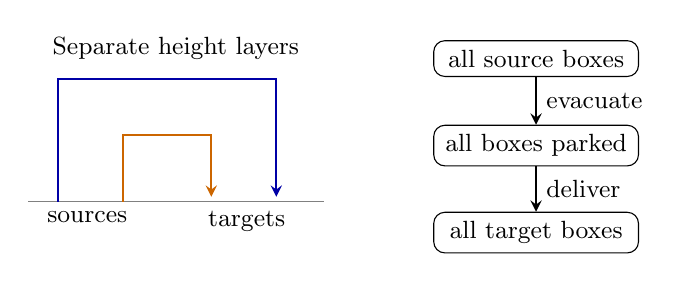
\begin{tikzpicture}[x=.75cm,y=.65cm,>=stealth,font=\small]
 \draw[gray] (0,0)--(5,0);
 \draw[thick,blue!65!black,->] (.5,0)--(.5,2.4)--(4.2,2.4)--(4.2,.1);
 \draw[thick,orange!80!black,->] (1.6,0)--(1.6,1.3)--(3.1,1.3)--(3.1,.1);
 \node[below] at (1,0) {sources};
 \node[below] at (3.7,0) {targets};
 \node[above] at (2.5,2.6) {Separate height layers};
 \begin{scope}[xshift=5.1cm]
  \node[draw,rounded corners,minimum width=2.6cm] (s) at (1.8,2.8) {all source boxes};
  \node[draw,rounded corners,minimum width=2.6cm] (p) at (1.8,1.1) {all boxes parked};
  \node[draw,rounded corners,minimum width=2.6cm] (t) at (1.8,-.6) {all target boxes};
  \draw[->,thick] (s)--(p) node[midway,right] {evacuate};
  \draw[->,thick] (p)--(t) node[midway,right] {deliver};
 \end{scope}
\end{tikzpicture}
\caption{The two separation mechanisms in
Lemma~\ref{lem:bb-lift-parking}.  Left: horizontal projections separate
the lift and descent, and distinct heights separate the transfer;
the second horizontal coordinate is suppressed.  Right: a temporal
schedule, not a spatial drawing.  Every source is removed before any
target is occupied, so overlap between the two families is harmless.}
\label{fig:bb-routing}
\end{figure}

There is also a useful stream-function implementation of the first
schedule.  Suppose $a_i,a_i'$ are the lower left corners of $P_i,Q_i$.
At height $z_i$, put $d_i=a_i'-a_i$, $b_i=\log\lambda_i$ and
$g_i(s)=a_i+sd_i$.  On a neighborhood of the swept rectangle use
\begin{equation}\label{eq:bb-mid-stream-path}
 \xi_i(s)=g_i(s)+\operatorname{diag}(\lambda_i^s,\lambda_i^{-s})(\xi-a_i).
\end{equation}
The Hamiltonian
\[
 H_i=d_{i1}y-d_{i2}x+b_i(x-g_{i1})(y-g_{i2})
\]
generates this motion. Put $\widehat H_i=\chi_iH_i$, where $\chi_i$
is one near the whole sweep and supported in its reserved layer. Use
\[
 \dot s(\partial_y\widehat H_i,-\partial_x\widehat H_i,0).
\]
Disjoint height layers separate these cutoffs.  Vertical phases use
$\nabla\times(0,x\chi_i,0)$, equal to $(0,0,1)$ on their column
plateaus.  If $M=\max_i(1,\lambda_i,\lambda_i^{-1})$ and the column
plateau margins are $\delta,\delta'$, an initial thickening smaller than
$\min(\delta/(4M),\delta'/(4M),1/(8M))$ stays on every plateau.
Thus the affine formula also holds on open neighborhoods. For points of
the original rectangle it has the additional bound
\begin{equation}\label{eq:bb-mid-stream-safe}
 X_1(s)\ge\min(a_{i1},a'_{i1}).
\end{equation}
The bound follows because the first relative coordinate in
\eqref{eq:bb-mid-stream-path} is nonnegative.

\subsection{Solid boxes with overlapping projections}

The preceding lift requires separate horizontal projections.  We now
remove that restriction; this is needed when all three coordinates
encode independent stacks.

\begin{theorem}[Expansion, obstacle detours, and delivery]
\label{lem:bb-balanced-box-routing}
Let $Q_i=a_i+\prod_{j=1}^3[-h_{ij},h_{ij}]$ and
$Q_i'=b_i+\prod_{j=1}^3[-k_{ij},k_{ij}]$ be rational solid boxes,
with positive half-widths, each family pairwise disjoint.  Suppose
$s_{ij}=k_{ij}/h_{ij}$ and $\prod_js_{ij}=1$.  An effective compactly
supported smooth solenoidal field, zero outside the time interval
$[1/4,3/4]$, has time-one map
\[
 a_i+y\longmapsto b_i+\operatorname{diag}(s_{i1},s_{i2},s_{i3})y
\]
on a neighborhood of each $Q_i$.
\end{theorem}
\begin{proof}\label{proof:bb-balanced-box-routing}
For an empty family take the zero field.  Otherwise let
$R=\max(1,h_{ij},k_{ij})$.  Choose a rational $\Lambda>10$ so that
centers in each of the lists $(\Lambda a_i)$ and $(\Lambda b_i)$
are separated by more than $20R$ in maximum norm.  This is possible
because distinct disjoint boxes have distinct centers.  Let
\[
 K=\max(4\Lambda,|\Lambda a_{i1}|,|\Lambda b_{i1}|),
 \qquad d_i=(K+30Ri,0,0).
\]
The $d_i$ are parking centers, separated from each other and both scaled
families by at least $30R$ in their first coordinate.

First multiply all source centers by a common factor increasing from
$1$ to $\Lambda$, while keeping shapes fixed.  Next change all shapes
at those separated centers by factors $s_{ij}^{\theta}$,
$0\le\theta\le1$.  Each half-width is the geometric interpolation
$h_{ij}^{1-\theta}k_{ij}^{\theta}\le R$.
Move the boxes one at a time from $\Lambda a_i$ to $d_i$, then,
after all have been parked, from $d_i$ to $\Lambda b_i$.
Finally shrink all target centers by a common factor from $\Lambda$
to $1$, with target shapes fixed.

Here is a finite construction of every single-box path.  Around each
stationary center place the closed cube of maximum-norm radius $4R$.
These cubes are disjoint since stationary centers are separated by
more than $20R$, and neither endpoint is in a cube.  Start with the
straight segment between the endpoints.  Its intersections with the
cubes are rational intervals, found by linear inequalities.  Replace
each portion inside a cube by a polygonal path on its boundary: join
the entry point to a vertex of a containing face, use cube edges to a
face containing the exit point, and join to that exit point.  The cube
is convex face by face, so these segments remain on its boundary;
no other cube meets them.  A tangency needs no replacement.  The
resulting rational polygonal path has distance at least $4R$ from
every stationary center.  Traverse its segments with flat switches,
stopping to all orders at vertices.  Its geometric image is unchanged,
so smoothing the time parameter does not reduce clearance.

For a uniform localization margin, let $g_a$ be the minimum over
$i<j$ of
\[
 \max_\ell(|a_{i\ell}-a_{j\ell}|-h_{i\ell}-h_{j\ell}),
\]
and define $g_b$ similarly.  These are positive; for a singleton list
set both to $R$.  During outward expansion a separating coordinate
gap can only increase; during final contraction the target gap is its
minimum.  During deformation centers are more than $20R$ apart.
During a single-box path the center distance is at least $4R$, leaving
a coordinate gap at least $2R$.  Hence padding smaller than
$\tfrac18\min(R,g_a,g_b)$ satisfies Lemma~\ref{lem:bb-curl}
throughout.  Put all stages, and all straight segments, in consecutive
subintervals of $[1/4,3/4]$.  Their flat switches give a smooth finite
motion, with positive diagonal determinant-one linear parts.  That
lemma provides the velocity and the neighborhood assertion.  All
choices use rational inequalities and effective elementary functions,
which also supply bounds for every derivative.
\end{proof}

\section{A complete balanced three-stack realization}\label{sec:bb-balanced-three-stack}

In a positional code with base $B$, replacing a prefix of length $r$
by one of length $s$ gives an affine map with slope $B^{r-s}$.
Thus a three-stack instruction has determinant one when it preserves
the sum of the three prefix lengths.  A third stack supplies reversible
history under this constraint: we first move a fresh blank from beyond
a work-tape boundary onto the history stack, then replace that blank
by the record.

\begin{theorem}[Balanced three-stack realization]
\label{thm:bb-balanced-three-stack}
For every machine and finite input, there are effective coefficients
$f_0,f_1$ such that $f=f_0+\nu f_1$ on $\R^3$ has an explicit
zero-data solution $(U,0)$.  Force and velocity have one compact
spatial support and bounded mixed derivatives of every order, and
are one-periodic after $t=1$.  At the fixed label $x_*=(4,0,0)$,
\[
 \exists t\ge0:\quad X(t;x_*)\in(-1,2)^3
 \quad\Longleftrightarrow\quad\text{the machine halts}.
\]
For a fixed machine its repeated field is independent of the input.
The comparison class is $u\in C H^2\cap C^1L^2$, bounded $u,\nabla u$
on finite intervals, and pressure modulo constants in $C H^1$.
The formula is valid for every fixed real $\nu>0$, with effective
evaluation when $\nu$ is computable and relative evaluation otherwise.
\end{theorem}
\begin{proof}
Normalize the finite machine to one halting state $h$, directing missing
nonhalting instructions to it by unchanged-letter stay moves. This preserves
initial halting as well. Let $\Gamma$ be the work alphabet and
$b\in\Gamma$ its blank. Use three infinite top-first stacks $L,R,J$.  A rule replaces three
finite prefixes, leaving their tails untouched.  Introduce boundary
$\star$, marked work letters $\bar a$, and controls $A_q,S_q,T_q,D_q$;
only $A_h$ is terminal.  For each $q\ne h$, the preparatory rules are
\begin{align}
 (A_q;\varepsilon,a,\varepsilon)&\to(S_q;\bar a,\varepsilon,\varepsilon),
 \label{eq:bb-balanced-entry}\\
 (S_q;\varepsilon,c,\varepsilon)&\to(S_q;c,\varepsilon,\varepsilon),
 \label{eq:bb-balanced-out-sweep}\\
 (S_q;\varepsilon,\star b,\varepsilon)&\to(T_q;\varepsilon,\star,b),
 \label{eq:bb-balanced-blank}\\
 (T_q;c,\varepsilon,\varepsilon)&\to(T_q;\varepsilon,c,\varepsilon),
 \label{eq:bb-balanced-return-sweep}\\
 (T_q;\bar a,\varepsilon,\varepsilon)&\to(D_q;\varepsilon,a,\varepsilon).
 \label{eq:bb-balanced-restore}
\end{align}
Here $a,c\in\Gamma$.  For $\delta(q,a)=(q',d,\sigma)$ add
\begin{equation}\label{eq:bb-balanced-step-table}
\begin{array}{c|c|c}
\sigma&\text{source}&\text{target}\\\hline
0&(D_q;\varepsilon,a,b)&(A_{q'};\varepsilon,d,\kappa)\\
-1&(D_q;c,a,b)&(A_{q'};\varepsilon,cd,\kappa)\quad(c\in\Gamma)\\
1&(D_q;\varepsilon,ac,b)&(A_{q'};d,c,\kappa)\quad(c\in\Gamma)\\
1&(D_q;\varepsilon,a\star b,b)&(A_{q'};d,b\star,\kappa).
\end{array}
\end{equation}
Every individual row occurrence, including its choice of $c$, receives
a distinct record symbol $\kappa$.

\emph{Full-domain separation and initialized behavior.}
\label{lem:bb-balanced-processor}\label{proof:bb-balanced-processor}
Every rule preserves total prefix length: it is one in the transfer
rows, two in the blank-supply row, and respectively two, three, three,
four in the final rows.  Source branches at $A_q$ test the right top;
at $S_q$ the right top separates work letters from the boundary;
at $T_q$ the left top separates work and marked letters.  At $D_q$
the right top fixes the work instruction, with the next right symbol
or left top separating its remaining branches.  Target branches at
$S_q$ have distinct marked or ordinary left tops; at $T_q$ distinct
boundary or ordinary right tops; at $D_q$ distinct restored $a$;
and at an $A$ control distinct history tops $\kappa$.
This proves separation for arbitrary independent tails.

Initialize
\[
 (A_{q_0};b^\infty,v\star b^\infty,b^\infty),\qquad
 v=\begin{cases}\omega,&\omega\ne\varepsilon,\\b,&\omega=\varepsilon.
 \end{cases}
\]
At a checkpoint, $L$ lists cells strictly left of the head and
$R=a_1\cdots a_m\star b^\infty$, $m\ge1$, lists the current cell
and a finite right block; beyond it the tape is blank.  $J$ contains
completed records, newest first.  The first rule marks $a_1$ while
moving it left; $m-1$ forward transfers expose $\star$.  The blank
row removes one filler blank beyond that boundary and pushes it on
$J$, without changing the infinite blank filler.  The reverse transfers
and restoration of $a_1$ restore exactly the original two work stacks.
The final rule replaces the fresh history blank by its record and
performs the work instruction.  A left move pops the next cell from
$L$; a right move with $m\ge2$ pops the current cell from $R$;
when $m=1$ the last row exposes a blank and retains a nonempty right
block.  Thus the invariant holds and one work step costs
$1+(m-1)+1+(m-1)+1+1=2m+2$ rules.  An initially halted input needs
none.  The records recover the head displacements as well.

\emph{From balanced words to solid boxes.}
Give the enlarged alphabet $\Sigma$ the odd digits
$1,3,\ldots,2|\Sigma|-1$ in base $B=2|\Sigma|+1$.
For a finite word $v$ put $e(v)=\sum_{j=1}^{|v|}d(v_j)B^{-j}$;
for an infinite stack $\xi$ put
$e(\xi)=\sum_{j\ge1}d(\xi_j)B^{-j}$.
The prefix interval is $I(v)=e(v)+[0,B^{-|v|}]$, with
$I(\varepsilon)=[0,1]$.  Every infinite tail satisfies
\[
 \frac1{B-1}\le e(\xi)\le\frac{2|\Sigma|-1}{B-1}<1,
\]
so its code lies strictly inside each applicable prefix interval.
Distinct incompatible prefixes have positive gaps, since digits differ
by at least two while the remaining interval has width at most one unit
in the differing place. Place control $s$ at
$o_s=(4i_s,0,0)$, with $i_{A_h}=0$ and distinct positive integers
for the others.  The code of $(s;L,R,J)$ is
$o_s+(e(L),e(R),e(J))$.
A rule with input prefixes $\alpha_1,\alpha_2,\alpha_3$
and output prefixes $\alpha'_1,\alpha'_2,\alpha'_3$ gives boxes
\[
 Q_i=o_s+\prod_jI(\alpha_j),\qquad
 Q_i'=o_{s'}+\prod_jI(\alpha'_j).
\]
Both families are separately disjoint by the preceding full-prefix
separation.  In control-relative coordinates their exact maps are
\begin{equation}\label{eq:bb-balanced-affine-rule}
 y_j=e(\alpha'_j)+B^{|\alpha_j|-|\alpha'_j|}
                    (x_j-e(\alpha_j)).
\end{equation}
The identity $e(\alpha\xi)=e(\alpha)+B^{-|\alpha|}e(\xi)$
proves their action on every code.  Initialized stacks are eventually
blank, with rational codes
$e(vb^\infty)=e(v)+B^{-|v|}d(b)/(B-1)$.
The affine determinant equals
$B^{\sum|\alpha_j|-\sum|\alpha'_j|}=1$, exactly by balance.
Apply Theorem~\ref{lem:bb-balanced-box-routing} to these full boxes.

\emph{Every intermediate time.}
All half-widths are at most $1/2$, so that lemma uses $R=1$.
Sources have first coordinate at least four, since no rule leaves
$A_h$.  Targets with nonhalt control have the same property.
For such a branch the initial expansion and final contraction preserve
first coordinate at least four.  During deformation its center has
first coordinate at least $4\Lambda$.  Every scaled halt target
center has first coordinate at most $\Lambda$, whereas the endpoints
of each nonhalt parking path have first coordinate at least
$4\Lambda$.  Since $\Lambda+4<4\Lambda$, the original segment
cannot meet an obstacle cube around a halt target.  Any encountered
obstacle has first coordinate at least $4\Lambda$, so its boundary
detour remains at least $4\Lambda-4$.  Subtracting a half-width at
most one still leaves first coordinate greater than two.  Hence
\begin{equation}\label{eq:bb-balanced-no-premature-event}
 \Phi_\tau(Q_i)\subset\{x_1>2\}\quad(0\le\tau\le1)
 \quad\text{for every branch with nonhalt target}.
\end{equation}
This includes delivery after halt targets have already been filled.

Finally load $x_*=(4,0,0)$ along the straight segment to the rational
initial code using the translation part of Lemma~\ref{lem:bb-curl}.
It avoids $(-1,2)^3$ for a nonhalt initial control.  Repeat the box
field from time one.  Induction at integer times applies the exact
full-box maps; the finite compiler cycles reach a code in $(0,1)^3$
precisely upon halting.  Equation~\eqref{eq:bb-balanced-no-premature-event}
excludes every intermediate false visit.  The residual proposition
gives the force and uniqueness; compact support gives all finite-slab
Sobolev conditions and uniformly bounded kinetic energy.  Every choice
was finite and effective, including the obstacle detours.  The input
enters only the first loading path, completing the proof.
\end{proof}

\section{History records and complete symbolic domains}
\label{sec:bb-frontiers}

The balanced-stack theorem is complete.  The remaining realizations
use alternative recorders with tape data in two coordinates.
A motion of boxes is invertible.  To use it for an ordinary machine,
we must retain whatever information an instruction erases.  We use
finite history records in the sense of reversible computation, but
prove the local inverses below: reversibility of the initialized
execution would not by itself separate the full boxes.

A work instruction is $r=(q,a)\mapsto(p_r,b_r,d_r)$, with
$d_r\in\{-1,0,1\}$.  The work tape is indexed by $\Z$, starts with
head zero, and has only finitely many prescribed nonblank cells.
Halting states have no outgoing work instruction.  Missing instructions
can be replaced by write-preserving stationary steps to a fresh halt
state.  Unless a construction explicitly adds a dummy initial step,
an initially halting state is already a halt checkpoint. When a construction
uses a single halting state $h$, merge the original halting states and
redirect their incoming transitions; this preserves initial halting. In
the recorder tables $Q$ is the work-state set and $\Gamma$ the work
alphabet. Radix bases are chosen from the full cell alphabet, including
all history and mark tracks.

\subsection{A one-cell code and its exact inverse test}

A partial one-cell table sends a control and a scanned letter to a
new control, a written letter, and a displacement.  Its two incoming
conditions are: the new control determines the displacement, and the
new control together with the written letter determines the entire
old control and read letter.

\begin{lemma}[From one-cell tables to closed rectangles]
\label{lem:bb-onecell}\label{lem:bb-mid-prefix}
Give an alphabet of size $m$ digits separated by at least two, between
$0$ and $B-2$.  Put
\[
E(A)=\sum_{j\ge1}d(A_j)B^{-j},\qquad
I(v)=\sum_{j=1}^{|v|}d(v_j)B^{-j}+[0,B^{-|v|}].
\]
For a head-relative tape $(a_j)_{j\in\Z}$ use the coordinates
\[
 (x,y)=\big(E(a_{-1}a_{-2}\cdots),E(a_0a_1\cdots)\big).
\]
After writing at cell zero, a displacement $e$ makes the old cell $e$
the new cell zero.
A deterministic partial one-cell table satisfying the incoming
conditions acts, after separate state translations, by a finite list
of reciprocal affine maps on full closed rectangles.  Each source
family and each target family is separately disjoint.  For a rule
reading $a$, writing $b$, and moving by $e$, the branches are
\begin{equation}\label{eq:bb-one-cell-branches}
\begin{array}{c|c|c|c}
e&\text{source}&\text{target}&(x',y')\\\hline
1 &[0,1]\times I(a)&I(b)\times[0,1]
 &((d(b)+x)/B,By-d(a))\\
0 &[0,1]\times I(a)&[0,1]\times I(b)
 &(x,y+(d(b)-d(a))/B)\\
-1&I(c)\times I(a)&[0,1]\times(d(c)+I(b))/B
 &(Bx-d(c),[d(c)+(d(b)+By-d(a))/B]/B).
\end{array}
\end{equation}
The last row is split over every letter $c$.  Each linear part is
$\operatorname{diag}(B^{-e},B^e)$.  With odd digits
$1,3,\ldots,2m-1$ and $B\in\{2m+1,2m+2\}$, every code lies in
the interior of its applicable rectangle, and unscaled within-family
gaps are at least $B^{-2}$.
\end{lemma}
\begin{proof}
The identity $E(aA)=(d(a)+E(A))/B$ gives all three formulas and their
action on the independent tails.  At the first differing digit,
incompatible prefix intervals have a positive gap: the digit difference
is at least two while the child interval has length one in that scale.
Thus the source state, read letter, and any left split separate sources.
At one target state the displacement is fixed.  For a right or stationary
move the written letter separates the relevant target coordinate;
for a left move the pair $(c,b)$ separates the two-letter prefix.
The incoming inverse condition rules out duplicates.  These arguments
concern the complete intervals, including their endpoints.
For odd digits the infinite tail lies between $1/(B-1)$ and
$(2m-1)/(B-1)<1$, proving interiority.  The longest target prefix has
length two, giving the asserted gap.  Uniformly scaling state squares
by $s$ scales gaps by $s$ and leaves the linear parts unchanged.
\end{proof}

\subsection{Moving the work head before recording}

We first place a frontier to the right of every possible work head.
A temporary mark lets the history excursion return to the correct
cell even though its length grows with the computation.

\begin{lemma}[Move-first recorder]
\label{lem:bb-movefirst}\label{lem:bb-mid-right-compiler}
There is an effective one-cell table satisfying the incoming conditions
whose checkpoint configurations simulate the work machine.  After
$n$ work steps its frontier is at $n+2$, its records occupy
$2,\ldots,n+1$, and its temporary marks are all zero.  Each nonhalting
checkpoint has a finite positive continuation to the next one, with
no intervening checkpoint.
\end{lemma}
\begin{proof}
Use letters $(c,\ell,j)$ with work letter $c$, history
$\ell\in\{e,F\}\sqcup\{r\}$ and mark $j\in\{0,1\}$.
The controls are $C_q,J_r,S_r,P_p,T_p$.  The complete partial table is
\[
\begin{array}{lll}
 C_q:(a,\ell,0)&\mapsto J_r:(b_r,\ell,0),d_r&\ell\ne F,\\
 J_r:(c,\ell,0)&\mapsto S_r:(c,\ell,1),1&\ell\ne F,\\
 S_r:(c,\ell,0)&\mapsto S_r:(c,\ell,0),1&\ell\ne F,\\
 S_r:(c,F,0)&\mapsto P_{p_r}:(c,r,0),1,&\\
 P_p:(c,e,0)&\mapsto T_p:(c,F,0),-1,&\\
 T_p:(c,\ell,0)&\mapsto T_p:(c,\ell,0),-1&\ell\ne F,\\
 T_p:(c,\ell,1)&\mapsto C_p:(c,\ell,0),0&\ell\ne F.
\end{array}
\]
Initialize the frontier at two, all other history empty, and all marks
zero.  At checkpoint $n$ the head satisfies $|h_n|\le n$.
The first row updates the work tape and moves to $h'\le n+1$, strictly
left of the frontier $f=n+2$.  The second row marks $h'$.  The forward
scan writes $r$ at $f$, puts a new frontier at $f+1$, and the backward
scan stops exactly at the mark, which it clears.  Its length is
$2(f-h')+4$, so it is finite and positive.  This proves the invariant
inductively, including the exact work update and halt equivalence.

For the full-domain inverse, $r$ recovers the old work pair into $J_r$;
mark one distinguishes entry into $S_r$ from its mark-zero loop;
a written record determines entry into $P_p$; a written $F$
distinguishes entry into $T_p$ from its loop; and entry into $C_p$
uniquely restores mark one.  Every destination has the single incoming
displacement displayed in the table.  No invariant on remote cells
was used.
\end{proof}

\subsection{Recording before the work-head displacement}

The next table leaves its mark at the old work head.  Its final step
performs the work displacement; storing that displacement in the
checkpoint control keeps incoming moves unambiguous.

\begin{lemma}[Direction-recording scan]
\label{lem:bb-direction}\label{lem:bb-mid-mark-compiler}
Let $D=\{-1,0,1\}$ and let $O$ be either a singleton or $\{0,1\}$.
An effective one-cell table on
$\Gamma\times(\{\bot,F\}\sqcup\mathcal R)\times\{0,1\}\times O$,
where $\mathcal R=\{(q,e,a):q\text{ nonhalting},e\in D,a\in\Gamma\}$,
satisfies the incoming conditions.  It preserves the $O$ track in
its physical cells.  Starting with frontier at one, its checkpoint
at work step $n$ has frontier $n+1$, records at $1,\ldots,n$, zero
marks, and the correct work configuration.  A step from head $i$
takes $5+2(n-i)$ local rules.
\end{lemma}
\begin{proof}\label{proof:bb-mid-mark-compiler}
Use main controls $M(q,e)$, forward controls $G(r)$, and $A(p,d),B(p,d)$
for every work state $p$ and $d\in D$, including pairs not produced by
a work instruction. Copy the $O$ component in each row. In the first
three rows use every $r=(q,e,a)\in\mathcal R$ with
$\delta(q,a)=(p,c,d)$. The final three rows apply independently to
every $(p,d)\in Q\times D$, including pairs that are not outputs of
any work instruction. The variables $v\in\Gamma$ and
$h\in\{\bot,F\}\sqcup\mathcal R$ range over all letters subject to
the displayed restrictions. The whole table is
\[
\begin{array}{lll}
 M(q,e):(a,h,0)&\mapsto G(r):(c,h,1),1&h\ne F,\\
 G(r):(v,h,0)&\mapsto G(r):(v,h,0),1&h\ne F,\\
 G(r):(v,F,0)&\mapsto A(p,d):(v,r,0),1,&\\
 A(p,d):(v,\bot,0)&\mapsto B(p,d):(v,F,0),-1,&\\
 B(p,d):(v,h,0)&\mapsto B(p,d):(v,h,0),-1&h\ne F,\\
 B(p,d):(v,h,1)&\mapsto M(p,d):(v,h,0),d&h\ne F.
\end{array}
\]
Starting at $M(q_0,0)$, the first row writes and marks the old head.
The scan reaches frontier $j=n+1$, stores its record, creates the
next frontier, returns to the unique mark and makes the work move.
The count is $2(j-i)+3=5+2(n-i)$.  Since $i\le n<j$, every test is
satisfied and both scans are finite.

Into $G(r)$ the written mark distinguishes entry and loop; $r$
recovers the old state and work symbol.  Into $A(p,d)$ the record
recovers the old $G(r)$.  Into $B(p,d)$ a written frontier distinguishes
arrival and loop.  Into $M(p,d)$ only clearing a mark is possible.
All remaining components were copied.  This proves the inverse on
arbitrary tapes and the fixed incoming displacement.  Deleting the
passive $O$ coordinate is an exact specialization of every rule,
not merely an equivalence of initialized runs.  When $O=\{0,1\}$,
a unique initial one at physical cell zero records the absolute origin.
\end{proof}

\subsection{A frontier on the left and post-halt continuation}

\begin{lemma}[Two left-frontier tables]\label{lem:bb-mid-left-compiler}
There are two effective incoming-separated tables: a stopping table,
and a table which continues with idle work steps after halting.
At checkpoint $n$ their frontier is $f_n=-2-n$ and their marks vanish.
If the next work move ends at $i'$, the next checkpoint is reached
after $4+2(i'-f_n)$ local rules.
\end{lemma}
\begin{proof}
For the stopping version let $J=(Q\setminus\{h\})\times\Gamma$.
For the continuing version take $J=Q\times\Gamma$ and add
$\delta(h,a)=(h,a,0)$.  Use letters
$(c,\eta,j)\in\Gamma\times(\{\bot,F\}\sqcup J)\times\{0,1\}$,
controls $C_q,D_q,T_q,P_r,S_r$, and precisely
\begin{equation}\label{eq:bb-mid-left-table}
\begin{aligned}
 C_q:(a,\eta,0)&\mapsto P_r:(b_r,\eta,0),d_r,\\
 P_r:(c,\eta,0)&\mapsto S_r:(c,\eta,1),-1&&\eta\ne F,\\
 S_r:(c,\eta,0)&\mapsto S_r:(c,\eta,0),-1&&\eta\ne F,\\
 S_r:(c,F,0)&\mapsto D_{p_r}:(c,r,0),-1,\\
 D_q:(c,\bot,0)&\mapsto T_q:(c,F,0),1,\\
 T_q:(c,\eta,0)&\mapsto T_q:(c,\eta,0),1&&\eta\ne F,\\
 T_q:(c,\eta,1)&\mapsto C_q:(c,\eta,0),0&&\eta\ne F.
\end{aligned}
\end{equation}
In the first row only, the stopping version requires $\eta\ne F$;
the continuing version allows every $\eta$.  These domains remain
distinct even though initialized runs never use that difference.

Initialize $F$ at $-2$, empty history elsewhere and zero marks.
At checkpoint $n$, $i\ge-n=f_n+2$.  After the work update,
$i'\ge f_n+1$.  Marking $i'$ and scanning left therefore reaches
$f_n$, records $r$, puts the next frontier at $f_n-1$, and returns
right to the mark without crossing the new frontier.  Clearing it
completes the next work checkpoint.  The two finite traversals and
four endpoint actions give the stated count.  The continuing version
has a next rule even after every halt checkpoint.

Into $P_r$ the record index recovers the work pair.  Into $S_r$
mark one distinguishes entry from loop; into $D_q$ the written record
recovers the scan; into $T_q$ a written $F$ distinguishes entry from
loop; into $C_q$ there is only stationary unmarking.  This proves the
incoming conditions for both full partial domains.  It also gives
the configuration inverse: reverse the displacement, inspect the
written cell, and invert its uniquely determined rule.
\end{proof}

\subsection{A guarded update on two neighboring history cells}

One may advance the frontier and write its record in a single local
instruction.  The resulting return loop needs a neighboring-cell guard.
Without that guard, its image would overlap the logging image.

\begin{lemma}[Three-cell guarded window]\label{lem:bb-window-compiler}
There is a finite partial injective map on relative tapes with controls
$\mathrm{Ready}(q,e)$, $\mathrm{Go}(r)$ and $\mathrm{Back}(q,d)$.
Here $r=(q,e,a)$ records an instruction, with
$\delta(q,a)=(p(r),b(r),d(r))$.
Use work, history and mark tracks $A,H,J$.  At cursor position $i$,
the Ready row has $a=A_i$ and $r=(q,e,a)$.  The entire table is
\[
\begin{array}{c|l|l}
\text{control}&\text{test}&\text{action}\\\hline
\mathrm{Ready}(q,e)&q\text{ nonhalting},J_i=0
 &A_i\gets b(r),\ J_i\gets1,\ \mathrm{Go}(r),+1\\
\mathrm{Go}(r)&J_i=0,H_i\ne P&\mathrm{Go}(r),+1\\
\mathrm{Go}(r)&J_i=0,H_i=P,H_{i+1}=E
 &H_i\gets r,H_{i+1}\gets P,\ \mathrm{Back}(p(r),d(r)),-1\\
\mathrm{Back}(q,d)&J_i=0,H_{i+1}\ne P&\mathrm{Back}(q,d),-1\\
\mathrm{Back}(q,d)&J_i=1&J_i\gets0,\ \mathrm{Ready}(q,d),d.
\end{array}
\]
Unmentioned cells and tracks are copied.  Initialized with frontier
at $r_0\in\{1,2\}$, other history $E$, zero marks and
$\mathrm{Ready}(q_0,0)$, the checkpoint at step $n$ has frontier
$p_n=n+r_0$ and correct head
$h_n$.  Its next work step uses exactly
$2(p_n-h_n)+1\le4n+2r_0+1$ local rules.
\end{lemma}
\begin{proof}
The first rule writes and marks $h_n$.  Since $p_n>h_n$,
the forward scan reaches the frontier, moves it one cell right, and
the return scan reaches the mark.  Its neighboring-cell guard holds
because the new frontier is $p_n+1$.  The last rule clears the mark
and performs the work displacement.  Counting the two traversals and
endpoint actions gives $2(p_n-h_n)+1$; induction gives $|h_n|\le n$.

For injectivity on all relative tapes, into Go the old cursor is
output offset $-1$: a mark there distinguishes entry from the loop,
and $r$ restores the overwritten work letter and old Ready control.
Into Back the old cursor is offset $+1$.  An output pointer at $+2$
identifies a log insertion, with record at $+1$ recovering $r$ and
old pair $(P,E)$.  A nonpointer at $+2$ identifies the guarded loop.
Into Ready the corresponding Back control uniquely restores the
cleared mark.  These are all possibilities, proving the full inverse.
\end{proof}

\begin{lemma}[Closed rectangles for a finite guarded window]
\label{lem:bb-window-rectangles}
Suppose a finite partial injective local tape map reads and writes only
indices $[-a,b-1]$, then shifts the cursor by $e$, where
$-a\le e\le b$.  Split its domain by every complete word in that
window.  With gapped radix coding the input prefix lengths are
$(a,b)$ and output lengths $(a+e,b-e)$; the affine branch has linear
part $\operatorname{diag}(B^{-e},B^e)$.  Both full rectangle families
are separately disjoint.
\end{lemma}
\begin{proof}
After the writes the new left prefix consists of old indices
$e-1,e-2,\ldots,-a$, and the right prefix of $e,e+1,\ldots,b-1$.
The two remaining tails are free and unchanged, so the image is the
whole output cylinder.  Distinct source cylinders have disjoint
images by injectivity.  If both pairs of output prefixes were
compatible, a common extension would belong to both images; hence
at least one coordinate has incompatible prefixes.  The gapped
interval argument then separates the complete closed rectangles.
The prefix lengths give the two reciprocal scales directly.
\end{proof}

\section{History conventions and branch subdivision}\label{ba:codes}

The general box motions now let us choose a recorder and an observer
separately.  We begin with the two frontier recorders in
Section~\ref{sec:bb-frontiers}, which retain history in the
sense of Bennett~\cite{Bennett1973}.  Later we retain the distinct
neighboring-cell guards and persistent-mark tables needed by other
realizations.  A full-domain inverse, not merely agreement along an
initialized run, is the criterion for sharing a compiler.

For these applications let $A$ be the work alphabet with distinguished
blank, $Q$ the states, $q_0$ the initial state, and $H\subseteq Q$
the halting states.  Write $h_n$ for the work head after $n$ steps and
\[
 \delta(q,a)=(q^+(r),b(r),d(r)),\qquad
 r=(q,a)\in\mathcal R=(Q\setminus H)\times A,
 \quad d(r)\in\{-1,0,1\}.
\]
The initial head is zero and the tape has finitely specified nonblank
cells.  Replace missing instructions by unchanged-letter stay moves to
a halt.  If one halt square is needed, merge halting states and redirect
their incoming instructions; no outgoing rule is changed.  This preserves
initial halting as well.  An unreachable halt state can be added when
needed.  These are the same normalizations as in
Section~\ref{sec:bb-frontiers}.

\subsection{Frontier recorders and their notation}

We use the move-first recorder of Lemma~\ref{lem:bb-movefirst}
with its original notation and complete partial domain.
The delayed-head recorder of Lemma~\ref{lem:bb-direction} records the
work displacement until its final return step.  Its table can also be
initialized with the frontier one cell farther to the right.

\begin{lemma}[Six-rule history recorder]\label{ba:six-compiler}
For $r_0=1$ or $r_0=2$, there is a partial table with the two incoming
properties of Lemma~\ref{lem:bb-onecell}, frontier $r_0+n$ at checkpoint
$n$, and checkpoint control recording both the work state and the
preceding work displacement.  Its next checkpoint takes
$2(r_0+n-h_n)+3$ instructions.  The work head moves only on the last
instruction.
\end{lemma}
\begin{proof}\label{ba:six-proof}
Specialize Lemma~\ref{lem:bb-direction} to a singleton passive track
$O$ and delete that coordinate.  Rename its controls
$(M(q,e),G(\tau),A(q,d),B(q,d))$ as
$(M_{q,e},R_\tau,F_{q,d},L_{q,d})$, and its frontier $F$ as $P$.
The full alphabet is
$A\times(\{\bot,P\}\sqcup\mathcal T)\times\{0,1\}$,
where $\mathcal T=(Q\setminus H)\times\{-1,0,1\}\times A$.
Every row and guard is the same under this bijection, so both incoming
properties hold on the entire partial domain, including unused controls.
Only $M_{q,e}$ with $q\in H$ are halting controls.

Initialize $M_{q_0,0}$ with all marks zero, frontier at $r_0$, and
empty history elsewhere.  The case $r_0=1$ is the initialization already
proved in the shared lemma.  For either allowed $r_0$, checkpoint $n$
has frontier $g=r_0+n>h_n$.  Mark the old head, scan right to $g$,
write the record and install the new frontier at $g+1$, then return to
the mark.  All intervening history is nonfrontier, the new frontier
cell is empty, and there is only one mark.  Hence the same rows apply
when $r_0=2$.  There are $g-h_n-1$ continuing right moves,
$g-h_n$ continuing left moves, and four other instructions, giving
$2(g-h_n)+3$.  The last row clears the mark and makes the work
movement; the invariant is restored with frontier $g+1$.  This proves
finite completion, indefinite legality for a nonhalting run, and the
stated halt equivalence, including initial halting.
\end{proof}

\subsection{From symbolic cylinders to closed rectangles}

Radix encodings turn a push or pop of a tape letter into an affine map;
this is the generalized-shift viewpoint of
Moore~\cite{Moore1990,Moore1991}.  The following calculation adds the
separation of full closed rectangles needed for smooth localization.

\begin{lemma}[Separated rectangle codes]\label{ba:rectangles}
Let a deterministic partial tape table on an alphabet $\Gamma$ of size
$m$ have the two incoming properties of Lemma~\ref{lem:bb-onecell}.
Assign distinct odd digits $e(a)\in\{1,3,\ldots,2m-1\}$ and choose
an integer $B\ge2m+1$.  Its local rules admit effective positive diagonal
affine maps of determinant one between finite families of closed planar
rectangles.  Sources are pairwise separated, as are targets.  Both the
minimal subdivision and the subdivision by both adjacent letters given
below realize every tape in their full symbolic cylinders.
\end{lemma}
\begin{proof}\label{ba:rectangles-proof}
Use Lemma~\ref{lem:bb-onecell} with digits $d(a)=e(a)$.  Its digit
hypotheses hold for every $B\ge2m+1$.  In the notation
\[
 C(a_1a_2\cdots)=\sum_{j\ge1}e(a_j)B^{-j},\quad
 h_a(v)=\frac{e(a)+v}{B},\quad
 I_{a_1\cdots a_l}=h_{a_1}\cdots h_{a_l}([0,1]),
\]
the left stream starts immediately left of the head and the right stream
starts at the head.  Place state $s$ in $k_s+a[0,1]^2$ with a common
rational $a>0$.  The minimal branch maps are exactly
\eqref{eq:bb-one-cell-branches}; scaling both charts by $a$ leaves
$\operatorname{diag}(B^{-d},B^d)$ unchanged.

For the additional full subdivision, restrict the right- and stay-move
sources to $x\in I_\gamma$, for every full letter $\gamma$.
Their targets become $I_{\beta\gamma}\times[0,1]$ and
$I_\gamma\times I_\beta$, respectively, for written letter $\beta$.
The already split left-move targets remain
$[0,1]\times I_{\gamma\beta}$.  At a fixed target state the
incoming direction is fixed, and the pair $(\beta,\gamma)$
distinguishes the branches in every case.  Thus the added subdivision
preserves separate target separation, while source separation follows
by restriction of the shared source rectangles.  All these statements
concern the filled closed rectangles and arbitrary symbolic tails.

For completeness the quantitative gaps remain valid for the entire
range $B\ge2m+1$: distinct first-digit intervals have gap at least
$B^{-1}$ and distinct second-digit intervals at least $B^{-2}$.
The source and target families therefore have within-state gaps at
least $aB^{-2}$; different state squares have their own chosen gaps.
Tail values lie between $1/(B-1)$ and $(2m-1)/(B-1)<1$.
An initial constant tail after $l$ digits contributes
$B^{-l}e(a_{\rm tail})/(B-1)$, so initialized codes are rational.
At checkpoints the history records, or the known absolute origin of
the record block, also recover the absolute work-head position.
\end{proof}


\subsection{Conventions for the remaining geometric realizations}\label{bc:section}
\label{bc:frontier-section}
Unless a different table is specified, subsequent routes use the move-first recorder of
Lemma~\ref{lem:bb-movefirst}, with initial frontier two. The controls
$(C_q,J_r,S_r,P_q,T_q)$ there are written $(W_q,P_r,B_r,C_q,D_q)$
here, and its empty/frontier/record symbols $(e,F,r)$ are written
$(E,F,R_r)$. Permuting work, history and mark coordinates in every row
preserves every guard. This identifies the full partial table, its inverse
and the exact checkpoint count $2(2+n-h')+4$, including arbitrary allowed
tapes. A nonterminal branch means one with both endpoint controls
nonterminal; a final branch into a halt can enter the observer.

The full branches are those of Lemma~\ref{lem:bb-onecell}. For an alphabet
of size $m$ we use one of the following explicitly indicated conventions:
\begin{equation}\label{bc:digits}
(B,\{d_a\})=(2m+2,\{1,3,\ldots,2m-1\}),\quad
(2m+1,\{1,3,\ldots,2m-1\}),\quad
(2m,\{0,2,\ldots,2m-2\}).
\end{equation}
All satisfy its digit bound and separation hypotheses. In the last
convention the full blank has digit zero; boundary codes remain in the
closed-rectangle and neighborhood conclusions. Write
$C(a_1a_2\cdots)=\sum_{j\ge1}d_{a_j}B^{-j}$ and
$I_v=\sum_{j=1}^{|v|}d_{v_j}B^{-j}+[0,B^{-|v|}]$.
A constant tail after $k$ positions contributes
$d_{\rm tail}B^{-k}/(B-1)$, so the initial codes are rational.
Guarded three-cell rules use Lemma~\ref{lem:bb-window-rectangles} with
$(a,b)=(1,2)$ after their own full-domain inverse has been proved.

\subsection{Analytic conventions for the geometric variants}\label{bc:analytic-section}
The whole-space baseline in these variants means smooth
$u\in CH^2\cap C^1L^2$, bounded $u,\nabla u$ on finite intervals,
and a pressure representative in $CH^1$. When the competitor-gradient
condition is omitted explicitly, the other conditions remain unchanged.
Both cases fall under Lemma~\ref{lem:b-comparison}(i); separately stated
pressure classes are retained. The torus baseline is its classical torus
clause. Unless a projection is specified, the force is
\begin{equation}\label{bc:residual}
f_U=U_t+(U\cdot\nabla)U-\nu\Delta U,\qquad (u,p)=(U,0).
\end{equation}
Torus projection is the separate choice in
Proposition~\ref{prop:projection-l2}, with changed pressure.
Localized affine motion is supplied by Lemma~\ref{lem:bb-curl} on a
compact time interval, using effective derivative bounds, positive lower
scale bounds and the positive cutoff margins specified in each route.
The potential is \eqref{eq:bb-potential}; the resulting flow fixes every
region disjoint from its support. In particular exponential diagonal
scales and linear reciprocal scales have respectively generators
$\theta'\log D$ and $\diag(l'/l,-l'/l,0)$.

\begin{lemma}[Finite forcing mechanisms]\label{bc:analytic}
A finite family of the preceding pulses, joined with flat time collars,
can be used once for initialization and repeated with period one thereafter.
It gives a smooth effective velocity and residual force with all mixed
derivatives uniformly bounded. In $\R^3$ both have one fixed compact
spatial support, and the velocity has uniformly bounded kinetic energy.
In a torus chart,
periodized curl or planar Hamiltonian pulses have zero spatial mean, as
does their residual force. Initial velocity and pressure are zero.
Uniqueness holds in the comparison classes of Section~\ref{sec:model};
in the whole-space class the competitor's gradient bound can be omitted
if the remaining conditions are retained.
\end{lemma}
\begin{proof}\label{bc:analytic-proof}
Each pulse is a finite expression in rational data, effective smooth
switches, their derivatives, positive diagonal scales and logarithms.
Finite positive separation margins bound every cutoff derivative. A finite
maximum bounds a period and the loading interval, and repetitions preserve
that bound. To evaluate near a join, a coarse enclosure of time gives a
finite superset of possibly active pulses. Summing them avoids an exact
comparison of a computable time with an integer. The flat collars give
smoothness. Compact support gives every required spatial Sobolev bound.
Lemma~\ref{lem:p2-realization} gives the asserted solution and comparison;
on a torus the integral of each curl or Hamiltonian derivative vanishes,
and the convection term is a divergence. Its flow satisfies
$\det D\Phi_t=1$, because differentiating this determinant gives
$(\divg U)(t,\Phi_t)\det D\Phi_t=0$ and its initial value is one.
The velocity and acceleration identities in that lemma consequently apply
to these volume-preserving diffeomorphisms.
\end{proof}

For later use, spatial chart changes are always made at the velocity level.
If $x=o+a y$, set $\widetilde U(t,x)=aU(t,(x-o)/a)$ and then compute
\eqref{bc:residual} at the prescribed physical $\nu$. The time and convection
terms scale by $a$, while the Laplacian term scales by $a^{-1}$.
Thus chart rescaling does not silently change the fixed physical viscosity.

\section{Affine motion on neighborhoods of boxes}\label{ba:geometry}

Rectangle separation controls the beginning and end of a transfer; distinct
heights separate its middle. We now specify the paths and cutoff margins
used by the applications. Interpolating one planar scale and its reciprocal
preserves thickness and, for a linear first scale, gives a convex formula
for each first coordinate. Interpolating both planar scales independently
gives that formula in both coordinates, at the cost of a compensating
normal strain during the motion.

\subsection{Reciprocal paths and their localization}
\label{sec:ba-localization}

Use the flat step $\sigma$ of \eqref{eq:p2-step} and put
\[
 \theta(s)=\sigma(2s-1/2),\qquad
 w_j(s)=\theta(3s-j+1)\quad(j=1,2,3).
\]
The switches $w_1,w_2,w_3$ perform the lift, horizontal transfer and
descent in separate thirds of the unit interval. All are constant near
their phase endpoints. The following version of
Lemma~\ref{lem:bb-lift-parking}(i) records a common vertical half-width
of one and explicit neighborhoods; the same formulas allow other heights
and thicknesses as described immediately afterward.

\begin{lemma}[Two explicit interpolations of separated boxes]
\label{ba:two-interpolations}
Let $S_i,T_i\subset\mathbb R^2$, $1\le i\le N$, be closed rational
rectangles of positive side lengths.  Suppose each list is pairwise
disjoint and
\[
 F_i(y)=c_i^T+\operatorname{diag}(\lambda_i,\lambda_i^{-1})(y-c_i^S),
 \qquad\lambda_i\in\mathbb Q_{>0},
\]
maps $S_i$ onto $T_i$, with $c_i^S,c_i^T$ their centers.  There is a
smooth nondecreasing switch $\eta:[0,1]\to[0,1]$, zero near 0 and one
near 1, for which either scale
path $r_i=\lambda_i^\eta$ or $r_i=1-\eta+\eta\lambda_i$ yields an
effective smooth compactly supported solenoidal unit-time field, zero
on time collars, realizing $(y,z)\mapsto(F_i(y),z)$ on the whole box
$S_i\times[-1,1]$ and a neighborhood of it.  The paths are affine;
each horizontal half-width remains between its endpoint values, and the
horizontal sweep of each original box lies in the coordinate bounding
rectangle of $S_i$ and $T_i$. With the linear choice, a particle's first
coordinate is the convex
interpolation of its endpoint first coordinates.
\end{lemma}

\begin{proof}\label{ba:two-interpolations-proof}
For $N=0$ take the zero field.  For $N\ge1$ apply
Lemma~\ref{lem:bb-lift-parking}(i) with vertical half-width one.
Use the shared phase switches with $\eta=w_2$ and set
\[
 C_i(s)=\big((1-\eta)c_i^S+\eta c_i^T,\,6i(w_1-w_3)\big),
 \qquad D_i(s)=\operatorname{diag}(r_i,r_i^{-1},1).
\]
The affine path is
$G_i(s,y)=C_i(s)+D_i(s)(y-(c_i^S,0))$.
Choose $\epsilon$ to be one quarter of the minimum of 1 and all
pairwise max-norm distances in the two planar lists, omitting empty
pair lists.  The $\epsilon$-padded moving boxes are disjoint: source
and target gaps are at least $4\epsilon$ during the vertical phases,
and the middle-phase height spacing is $6>2(1+\epsilon)$.

For later loading formulas, record the centered cutoff explicitly:
\[
 \chi(C,L,\epsilon;x)=
 \prod_{j=1}^3\sigma\!\left(\frac{L_j+\epsilon+x_j-C_j}{\epsilon/2}\right)
 \sigma\!\left(\frac{L_j+\epsilon-x_j+C_j}{\epsilon/2}\right).
\]
Here $L$ is the vector of half-widths; the plateau has padding
$\epsilon/2$ and the support has padding $\epsilon$.
If $L_i(s)$ are the moving half-widths, $Y=x-C_i(s)$ and
$A_i=D_i'D_i^{-1}$, the field supplied by
\eqref{eq:bb-potential} is
\begin{equation}\label{ba:affine-box-field}
 V(s,x)=\sum_i\nabla\times\left\{
 \chi(C_i,L_i,\epsilon;x)
 \left[\tfrac12 C_i'\times Y+\tfrac13(A_iY)\times Y\right]
 \right\}.
\end{equation}
Indeed $\det D_i=1$, and the preceding separation verifies
Lemma~\ref{lem:bb-curl} with localization parameter $\epsilon/2$.
Its neighborhood conclusion applies with
$L_* =\max_i\max(1,\lambda_i,\lambda_i^{-1})$ because
$\|D_i(s)\|_\infty\le L_*$ and $D_i(0)=I$.
It therefore gives the stated affine motion on the full boxes and
on their initial max-norm neighborhoods of radius $\epsilon/(4L_*)$.
The paths are stationary for $s\le1/12$ and $s\ge11/12$.
Their finite center ranges and endpoint width bounds give common
compact support.  The effective positive lower bound
$r_i\ge\min(1,\lambda_i)$ verifies the scale requirement.
For the linear scale, the first-coordinate identity is
\[
 (G_i(s,y))_1=(1-\eta)y_1+\eta(F_i(y_1,y_2))_1.
\]
The second coordinate need not interpolate its own endpoint values.
Instead, if $b_{i2}$ is the source's second half-width, convexity of the
reciprocal function gives
\begin{equation}\label{eq:ba-reciprocal-envelope}
 \frac{b_{i2}}{(1-\eta)+\eta\lambda_i}
 \le (1-\eta)b_{i2}+\eta\frac{b_{i2}}{\lambda_i}.
\end{equation}
The first half-width is exactly its endpoint interpolation. For the
exponential scale, convexity of the exponential gives the corresponding
upper bounds in both coordinates, since
$\lambda_i^{\pm\eta}\le(1-\eta)+\eta\lambda_i^{\pm1}$.
In either case the center is interpolated linearly and each half-width
is at most the interpolation of its endpoint half-widths. Therefore each
lower edge is at least the interpolation of the endpoint lower edges,
and each upper edge is at most the corresponding interpolation of upper
edges. This proves the claimed bounding rectangle for the entire sweep.
The individual endpoint-width bounds also follow directly from monotonicity
of the positive scales and their reciprocals.
\end{proof}

The same construction applies to $P_i\times[-h,h]$ for any common
$h\ge0$, including plates and rectangles with zero side lengths, under
the hypotheses of Lemma~\ref{lem:bb-lift-parking}(i). Replace $6i$ by
heights $H_i$ whose pairwise gaps exceed $2h+2\varepsilon$, and choose
$\varepsilon$ below one third of every within-family planar gap. The
formula for $C_i$ uses the source and target centers in place of
$c_i^S,c_i^T$; its support padding is $\varepsilon$ and plateau padding
is $\varepsilon/2$. Source projections, distinct heights and target
projections separate the three phases in that order. Empty pair lists
impose no gap restriction, and the empty family gives the zero field.
Arbitrary real data give smooth existence; the effective-data assumptions
of the shared lemma give computable scales, derivative bounds and margins.
The same perturbation argument gives an open neighborhood even when a
side length is zero.

\subsection{Transporting an initial cutoff}
\label{sec:ba-transported-localization}

The transported-initial-cutoff convention is also useful.  Write the
affine path as $G_i(t)x=J_i(t)x+g_i(t)$ and localize by
$\psi_i(G_i(t)^{-1}x)$, where $\psi_i$ has support padding
$\varepsilon_0$ around the initial box and equals one on a smaller
positive padding.
If $\lambda_i\in[B^{-1},B]$, its initial padding
$\varepsilon_0$ expands horizontally by at most $B$.  Choose
$2B\varepsilon_0$ below every target gap,
$2\varepsilon_0$ below every source gap, and
$\varepsilon_0\le\varepsilon$.  These transported supports stay
separated in the same three phases.  The affine generator is
$v_i+A_ix$, with $A_i=\dot J_iJ_i^{-1}$ and
$v_i=\dot g_i-A_ig_i$.  Its potential is
\[
 \tfrac12v_i\times x+\tfrac13(A_ix)\times x.
\]
The identity proved in Lemma~\ref{lem:bb-curl} gives the exact
generator on the transported plateau.  Its neighborhood argument then
proves the same full-box endpoint map.  The factor $B$ in the margin
choice is essential: transported padding does not stay fixed under
stretching.

\subsection{Independent planar interpolation}

For an observer that needs both planar coordinates to follow their own
endpoint interpolations, the reciprocal path is insufficient. The next
construction interpolates the two factors independently and compensates
the temporary planar area change in the third direction. Here the named
targets may be disjoint containers of the actual affine images; only the
image centers enter the motion.

\begin{lemma}[Independent planar scales and normal compensation]
\label{ba:plate-routing}
Let $P_i,Q_i\subset\R^2$ be finite families of closed rectangles,
separately pairwise disjoint, and let assigned positive diagonal affine
maps $F_i$ satisfy $F_i(P_i)\subseteq Q_i$. Write their diagonal factors as
$\lambda_{i1}^*,\lambda_{i2}^*>0$ with product one.
There is a smooth compactly supported solenoidal unit-time field, zero on
time collars, whose endpoint map is $(y,z)\mapsto(F_i(y),z)$ on a
neighborhood of each entire plate $P_i\times\{0\}$. During the horizontal
phase both planar factors interpolate linearly, while the normal factor
compensates their product. Each planar coordinate of a point on the plate
is its convex endpoint interpolation.
\end{lemma}
\begin{proof}\label{ba:plate-routing-proof}
Use the height phases in Section~\ref{sec:ba-localization}. For source
center $p_i$, end its center path at its actual image $F_i(p_i)$; in the
onto case this is the named target center. Choose separated heights $H_i$
as above and set
\[
 c_i=\bigl((1-w_2)p_i+w_2F_i(p_i),\,H_i(w_1-w_3)\bigr),
\]
\[
 \lambda_{ij}=1-w_2+w_2\lambda_{ij}^*,\qquad
 D_i=\operatorname{diag}\bigl(
 \lambda_{i1},\lambda_{i2},(\lambda_{i1}\lambda_{i2})^{-1}\bigr).
\]
The volume-preserving path has logarithmic derivative
\[
 T_i=\dot D_iD_i^{-1}=\operatorname{diag}\left(
 \frac{\dot\lambda_{i1}}{\lambda_{i1}},
 \frac{\dot\lambda_{i2}}{\lambda_{i2}},
 -\frac{\dot\lambda_{i1}}{\lambda_{i1}}
 -\frac{\dot\lambda_{i2}}{\lambda_{i2}}\right).
\]
This matrix has trace zero, so \eqref{eq:bb-potential} localized
around the moving plate gives the desired field.  Its planar motion is
$c_i+(\lambda_{i1}(y_1-p_{i1}),\lambda_{i2}(y_2-p_{i2}),0)$.
Normal displacement changes by the factor
$(\lambda_{i1}\lambda_{i2})^{-1}$. The factors have positive
lower bounds; choose the initial thickness less than their product's
minimum times the normal plateau width.  A small enlargement of the
planar rectangle is allowed by the positive collars as well.  Thus a
whole thin neighborhood follows the volume-preserving affine motion.
The normal factor returns to one at the endpoint. The final plate image
is contained in $Q_i\times\{0\}$. Source and target-container
gaps protect the vertical phases and distinct heights protect the
middle phase.  Linear interpolation of each planar factor gives both
convex-coordinate identities on the plate.
This proves smooth existence for arbitrary real data. Under the effective
input assumptions of Lemma~\ref{lem:bb-curl}, the positive scale bounds and
finite gap margins can be computed and the construction is effective.
\end{proof}

\subsection{Forcing and effective evaluation}

\begin{lemma}[Residual forcing for the finite processors]\label{ba:realization}
Fix computable $\nu>0$.  Let $W$ be smooth, solenoidal, initially zero,
with support in one compact subset of $\mathbb R^3$ and every mixed
derivative bounded.  Then
\begin{equation}\label{ba:residual}
 F_W=W_t+(W\cdot\nabla)W-\nu\Delta W
\end{equation}
has the same support and derivative properties.  The zero-data solution
$(W,0)$ is unique among smooth solutions with
$u\in C_tH^2\cap C_t^1L^2$, bounded $u$ on finite intervals, and
$p\in C_tH^1$.  The corresponding torus assertion holds in the
classical comparison class of Section~\ref{sec:model}.  A sum of curls
in a torus chart gives both $W$ and $F_W$ mean zero.  Finite formulas
from the effective-data instances of the preceding constructions, finite
loading, and repetition of one cycle give effective evaluation of every
force derivative.
\end{lemma}
\begin{proof}\label{ba:realization-proof}
Fixed compact support and bounded mixed derivatives imply all reference
velocity hypotheses of Lemma~\ref{lem:b-comparison}.  Case (i) gives
exactly the stated whole-space comparison class, without a competing
gradient bound; its torus clause gives the stated classical comparison
class.  The same lemma provides the pressure normalization and global
material flow.  The product rule applied to \eqref{ba:residual}
proves the force's support and derivative bounds.  A chart curl has
zero mean, and integration of the residual uses
$\int\Delta W=0$ and
$\int(W\cdot\nabla)W=\int\operatorname{div}(W\otimes W)=0$.
For these effective-data instances, gate derivatives and seam evaluation are
those of \eqref{eq:p2-step} and Proposition~\ref{prop:bb-realization}.
The explicit affine scales and every reciprocal denominator have positive
computable bounds.  Thus differentiating the finite formulas, using a
finite superset of possible period indices, evaluates every derivative
without a machine execution or a real equality test at a seam.
\end{proof}

\section{Choosing initialization and the observer}
\label{sec:bb-initialization}

The preceding recorders supply complete instruction tables. We now
specify how their boxes are positioned and how the fixed material label
becomes the initial code. We compare one-time loading, a loading branch
repeated in every cycle, and chart translations that place the initial
code at the label itself. The latter two choices can preserve periodicity
from time zero. Each construction also needs a bound between integer
rule times; the endpoint coding alone does not give a material event.

Unless stated otherwise, the force in this section is the residual
\eqref{eq:bb-residual}, with pressure zero.  Its smoothness, all-order
mixed derivative bounds, finite effective prescription and uniqueness
are as in Proposition~\ref{prop:bb-realization}.  Whole-space forces
have one compact spatial support; torus forces have zero spatial mean.
All statements use a fixed positive computable viscosity, with the
relative interpretation of that proposition for arbitrary fixed
positive viscosity.

\subsection{Torus loading and direct chart placement}

\begin{proposition}[A move-first material test]\label{thm:bb-torus33}
The move-first recorder has a unit-torus realization, periodic after
$t=1$, whose fixed label $(1/4,1/2,1/4)$ enters
$\{x_1\in(1/2,1)\pmod1\}$ exactly when the work machine halts.
For a fixed machine only the loading interval depends on the input.
\end{proposition}
\begin{proof}\label{proof:bb-torus33}
Use Lemma~\ref{lem:bb-movefirst}, let $\Sigma$ be its full cell alphabet,
and enumerate its $N$ controls by $i=1,\ldots,N$.
Set $s=1/[16(N+1)]$ and give the $i$th control a square
of side $s$ centered at
\[
 m_i=(o_i+i/[4(N+1)],1/2),\qquad
 o_i=\begin{cases}5/8,&C_q\text{ with }q\text{ halting},\\1/8,&\text{otherwise}.
 \end{cases}
\]
Use odd digits and $B=2|\Sigma|+2$.  The code at height $z_0=1/4$
is $(m_i+s(E(L)-1/2,E(R)-1/2),z_0)$.
It is rational initially.  Lemma~\ref{lem:bb-onecell} gives $J$
branches with separately separated rectangles, all side lengths at
most $s$ and endpoints on the grid of mesh
$[32(N+1)B^2]^{-1}$.  For branch $j$ choose height
$z_j=1/2+j/[4(J+1)]$.  Use the three-phase lift of
Lemma~\ref{lem:bb-lift-parking}, with exponential middle scale
$\lambda_j^\theta$ and center interpolation.  A padding parameter
\[
 \epsilon=\min\{1/128,[320(N+1)B^2]^{-1},[40(J+1)]^{-1}\}
\]
separates the enlarged sheets in the source, height, and target phases
and keeps them inside the unit cube.  Their thickness may then be
chosen positive by Lemma~\ref{lem:bb-curl}.  For $J=0$ the repeated
field is zero.

During $[0,1]$ a localized curl translation takes the fixed label
along the segment to the initial code.  Both segment and a small
padding lie in the chart.  Repeat the branch pulse thereafter.
At each subsequent integer time the particle is the next table code.
If both endpoint controls are nonhalting, the interpolated center and
half-width bounds give $x_1<3/8+s<1/2$ throughout the motion.
The loader also stays below $1/2$ in a nonhalting run.  A halting
checkpoint lies in the upper half, reached in finitely many positive
local steps; an initial halt is reached at the end of loading.
This proves the event for every real time.
\end{proof}

\begin{proposition}[A guarded-window material test]\label{thm:bb-window37}
The table of Lemma~\ref{lem:bb-window-compiler} has a unit-torus
realization, periodic after $t=1$, with fixed label $(1/4,1/4,1/4)$
and event $x_1\in(1/2,7/8)\pmod1$, occurring exactly when the
work machine halts.  At work step $n$ its next
checkpoint occurs after exactly $2(p_n-h_n)+1\le4n+5$ unit periods.
\end{proposition}
\begin{proof}\label{proof:bb-window37}
Choose $r_0=2$ in Lemma~\ref{lem:bb-window-compiler}: initially the
frontier is at cell two, all other history cells are empty, and all
marks are zero. Thus $p_n=n+2$, with records in cells $2,\ldots,n+1$.
Split the full three-cell windows $[-1,1]$ and apply
Lemma~\ref{lem:bb-window-rectangles} with $(a,b)=(1,2)$.
Let $\mathcal A$ be the full cell alphabet of this window table and use
odd digits in base $B=2|\mathcal A|+1$.
For $S$ controls let $\epsilon=1/[16(S+1)]$ and place their squares
at $o_s+\epsilon[0,1]^2$, where
\[
 o_s=(\xi_s,1/4+2\kappa(s)\epsilon),\quad
 \kappa(s)\in\{1,\ldots,S\},\quad
 \xi_s=\begin{cases}5/8,&s\text{ halting Ready},\\1/4,&\text{otherwise}.
 \end{cases}
\]
Write $J$ for the number of branches and $e_j$ for branch $j$'s cursor
displacement. The full source and target rectangle gaps are at least
$\epsilon B^{-3}$.  Put their common height at $1/4$, assign branch
$j$ height $1/2+j/[4(J+1)]$, and use the exponential middle scale
$\operatorname{diag}(B^{-e_j\theta},B^{e_j\theta},1)$.
Take one tenth of
$\min(1/32,\epsilon B^{-3},1/[4(J+1)])$ as padding.
Horizontal source and target gaps and the private heights separate
the three phases, while all widths remain at most $\epsilon$.
The strain can equivalently be generated by
$(0,0,-e_j\dot\theta\log B\,(x_1-c_{j1})(x_2-c_{j2}))$,
retaining the explicit diagonal-strain implementation.

A first unit interval loads the label along the segment to the rational
initial code.  Thereafter the exact rectangle action and the compiler
lemma give checkpoint times $t_0=1$ and
$t_{n+1}=t_n+2(p_n-h_n)+1$.  A nonhalting center stays in
$[1/4,1/4+\epsilon]$, with half-width at most $\epsilon/2$;
thus every intermediate first coordinate remains below $1/2$.
The loader has the same exclusion.  Halt codes are in
$[5/8,5/8+\epsilon]$, inside the observer, including an initial halt.
The history block starts at the known absolute cell two, so the
head-relative code also recovers absolute indexing at checkpoints.
\end{proof}

\begin{proposition}[Two direction-recording placements]
\label{thm:bb-aligned38}\label{thm:bb-direction39}
The direction recorder gives both of the following realizations.
\begin{enumerate}
\item On $\R^3$, with its passive origin bit, there is a force periodic
from time zero and a fixed-origin event $X_1(t;0)<-5$.  Input dependence
can be confined to two translations of the state charts.  On every
implemented full box the first coordinate is a convex combination
of its endpoint first coordinates.
\item On the unit torus, without the passive track, a force periodic
after $t=1$ has fixed label $(1/8,1/8,1/4)$ and event
$x_1\in(1/2,7/8)\pmod1$.  For a fixed machine its repeated part is
independent of the input.
\end{enumerate}
Both events are equivalent to halting.
\end{proposition}
\begin{proof}\label{proof:bb-aligned38}\label{proof:bb-direction39}
For the first case introduce a fresh terminal state $\dagger$ and
replace every missing instruction and every originally terminal
state--symbol pair by a write-preserving stationary transition into it.
The original initial control is therefore nonterminal in this normalized
table, even when the original machine is initially halted. Apply
Lemma~\ref{lem:bb-direction} with its passive origin track, and let
$\mathcal A$ be the resulting full cell alphabet. Use odd digits in
base $B=2|\mathcal A|+1$
and initial fractions $x_*,y_*$.  Index the initial main state by zero,
the main $\dagger$ states by distinct negative integers, and the rest
by distinct positive integers.  State $s$ has placement
\[
 (x,y)\longmapsto(10k(s)+x-x_*,y-y_*).
\]
The initialized point is zero; nonhalt codes have first coordinate
$>-1$, and halt codes $<-5$.  Thicken the rectangles of
Lemma~\ref{lem:bb-onecell} by $[-1,1]$, give branch $i$ height $10i$,
and use the linear scale $g_i=1+\theta(\lambda_i-1)$ in the lift
schedule.  A padding smaller than one tenth of the minimum of one
and all within-family planar gaps suffices.  The middle strain has
potential $(0,0,(\dot g_i/g_i)(x_1-c_{i1})(x_2-c_{i2}))$.
Equation~\eqref{eq:bb-convex-coordinate} excludes every nonhalting
visit to $x_1<-5$.  The table and routing are fixed for the machine;
only $x_*,y_*$ change with the input.  The passive origin bit remains
at physical cell zero, so no absolute tape information is discarded.

For the second case first merge all halting work states into a single
state $q_h$, redirecting incoming transitions and retaining initial halting.
Delete the passive track from the direction recorder, and now let
$\mathcal A$ denote that full alphabet. Use odd digits with
$B=2|\mathcal A|+2$ and
$\lambda=1/[16(J+1)]$, where $J$ counts the controls.  Number them
from zero and set
\[
 S_s(x,y)=(A_s+\lambda x,1/4+\lambda y),\qquad
 A_s=2\lambda\operatorname{index}(s)+
 \begin{cases}5/8,&s=M(q_h,e),\\1/4,&\text{otherwise}.
 \end{cases}
\]
The nonhalt squares lie in $[1/4,3/8]\times[1/4,1/4+\lambda]$;
halt squares lie in $[5/8,3/4]\times[1/4,1/4+\lambda]$.
Write $m$ for the number of branches. Use coding height $1/4$,
branch heights $1/2+i/[4(m+1)]$, and
the same linear first scale.  One hundredth of the minimum of
$1/16$, $1/[4(m+1)]$, and the source and target planar gaps is
valid padding; absent pair gaps are omitted.  All supports lie inside
the cube, and all horizontal widths are at most $\lambda$.
A localized translation with padding $1/1000$ loads the rational
initial point from the fixed label in one unit interval.

In a nonhalting period the center has first coordinate at most $3/8$
and half-width at most $\lambda/2$, hence is below $1/2$; loading
has the same bound.  Halting codes lie in the observer.  The exact
sampling induction gives one table step per period, with checkpoint
cycle $2(k+1-h_k)+3$.  The record block beginning at cell one
recovers absolute indexing at checkpoints.  An initial halt is
observed at time one.
\end{proof}


\subsection{A one-time torus loader}

The next placement uses a separate first interval to load the code. Only
the instruction cycle is then repeated, so periodicity begins at time one.

\begin{theorem}[A separate one-unit loader on the torus]
\label{ba:loaded-torus}
For every machine and finite input and every fixed computable $\nu>0$,
there is an effective smooth
mean-zero force, one-periodic for $t\ge1$ with bounded mixed derivatives,
whose unique smooth zero-data solution with zero normalized pressure
satisfies
\[
 \exists t\ge0:\ \Phi_t(1/2,1/2,1/4)
       \in(1/16,1/4)\times\mathbb T^2
 \quad\Longleftrightarrow\quad\text{halting}.
\]
Uniqueness holds in the classical class of Section~\ref{sec:model}.
\end{theorem}
\begin{proof}\label{ba:loaded-torus-proof}
Use the single-halt move-first recorder of
Lemma~\ref{lem:bb-movefirst}, without an entry state.  Let
$\Gamma$ be its full alphabet and $N$ its number of controls.  Put
$B=2|\Gamma|+1$, $a=1/(16N)$, the halt square at
$(1/8,1/4)+a[0,1]^2$, and the other squares at
$(1/2+2ja,1/4)+a[0,1]^2$, $0\le j\le N-2$.
Use the minimal subdivision, so right and stay moves are not split by
the left letter.  Its gaps are at least $a/B^2$.
For $M$ branches choose
\[
 h=\frac1{64(M+1)},\quad Z_i=\frac12+\frac{i}{4(M+1)},\quad
 \varepsilon=\min\{1/128,h/4,a/(4B^2)\}.
\]
Apply linear-first-scale full-box routing from height $z_0=1/4$.
Middle heights differ by $16h$; source and target gaps handle the
vertical phases.  Centers lie in
$[1/8,5/8]\times[1/4,5/16]$, widths are at most $a$, and all padded
boxes lie in $(1/16,15/16)^3$.  This is a construction on the specified
unit torus, with no change of physical viscosity.

In the first unit interval translate a box of side $1/64$ from the
fixed label to the rational initial code, using Lemma~\ref{lem:bb-curl}.
The segment and a small padding lie inside the same chart.  Repeat
only the instruction cycle afterward.  Code induction proves the
checkpoint identities.  A halting code has first coordinate in
$[1/8,3/16]$, including an initial halt reached by loading.  For a
nonhalting run both centers of every used branch have first coordinate
at least $1/2$, with half-width at most $a/2$; loading has the same
lower center bound.  Hence the particle always stays to the right of
$1/4$.  Residual realization proves every analytic assertion.  The
separate loading field accounts for the qualification $t\ge1$ in the
periodicity statement.
\end{proof}


\subsection{Repeated torus loading branches}\label{ba:torus}

A loader can instead be one branch of every period. To keep its target
separate from all computational targets, place the initial code in a state
square with no incoming instruction. This condition concerns the entire
target family, not only the distinguished execution. We implement the
same startup principle first with full boxes, then with fixed columns.

\begin{theorem}[A loader repeated as part of the processor]
\label{ba:periodic-torus}
For every finite machine and input, and every fixed computable $\nu>0$,
there is an effective smooth mean-zero force on the unit flat torus,
one-periodic from time zero, with all mixed derivatives bounded.  Its
zero-data solution has pressure zero, is unique in the classical class
of Section~\ref{sec:model}, and satisfies
\[
 \exists t\ge0:\ \Phi_t(1/8,1/8,1/4)
             \in\{5/8<X_1<7/8\}
 \quad\Longleftrightarrow\quad\text{the machine halts}.
\]
The one repeated cycle implements all instruction branches and its
loading branch.
\end{theorem}
\begin{proof}\label{ba:periodic-torus-proof}
Normalize to one halt state and prepend a new nonhalting state $q_I$
whose rule preserves the scanned letter, stays, and enters the original
initial state.  No machine rule targets $q_I$.  Apply the move-first
recorder of Lemma~\ref{lem:bb-movefirst} and omit the unused controls
$P_{q_I},T_{q_I}$. Then the entry control $C_{q_I}$ has no incoming local
instruction.  Write $\Gamma$
for this recorder's full alphabet.  Put $B=2|\Gamma|+1$, let $N$
be the number of controls, and set
$a=1/(16(N+1))$.  Use the halt square
$(3/4,1/4)+a[0,1]^2$ and nonhalting squares
$(1/4+2al,1/4)+a[0,1]^2$, $0\le l\le N-2$.
The full subdivision of Lemma~\ref{ba:rectangles} gives source
half-widths $a/(2B)$ in both coordinates.

Add a square with those half-widths centered at $(1/8,1/8)$ and a
translation to the square centered at the initial entry code.  Each
initial tail is at distance at least $1/(B-1)>1/(2B)$ from the endpoints
of $[0,1]$, so the new target lies strictly inside the entry square.
There is no other target in that square.  Both enlarged branch lists
therefore remain separately separated, with gaps at least $a/B^2$.
The extra source is separated from all state squares.

Number the branches, including loading, by $1\le i\le M$.  Set
\[
 z_0=\tfrac14,\qquad h=\frac1{16(M+1)},\qquad
 Z_i=\tfrac12+\frac{i}{4(M+1)},\qquad
 \varepsilon=\frac1{10}\min(h,a/B^2).
\]
Thicken each planar source by $[z_0-h,z_0+h]$.  Lift the resulting
full box to center height $Z_i$, move it horizontally, and lower it
to $z_0$.  For an instruction with displacement $d_i$, use
$D_i=\operatorname{diag}(B^{-d_iw_2},B^{d_iw_2},1)$;
loading has $d_i=0$.  Its center is the planar endpoint interpolation
plus $(Z_i-z_0)(w_1-w_3)e_3$.  Adjacent middle heights are $4h$ apart,
while the padded half-thickness is $h+\varepsilon<2h$.
Source and target gaps handle the other phases.  Horizontal half-widths
never exceed $a/2$, horizontal centers lie between $1/8$ and $3/4+a$,
and vertical centers lie between $1/4$ and $3/4$.  The padded motions
are thus strictly inside the unit cube.  Lemma~\ref{lem:bb-curl} gives a
chart field, extended periodically in space and time.  Its zero time
collars give zero initial velocity.

The first cycle loads the fixed particle.  Each subsequent cycle maps
its exact code to the next local code until the first halt, or forever
in a nonhalting run.  Lemma~\ref{lem:bb-movefirst} identifies the finite
checkpoint times with machine steps.  The added entry state handles an
original initial halt.  A halt code is in the target slab.  For a
nonhalting execution every used source and target center, including the
loader, has first coordinate at most $3/8$.  Exponential interpolation
keeps the center below that bound and the half-width below $a/2$;
the particle cannot reach $5/8$ at any intermediate time.  The final
transition into a halt is not subject to this nonhalting-endpoint bound.
Lemma~\ref{ba:realization} gives the force, its mean, its effective
derivatives, and uniqueness.  Repeating the loading field is harmless
to the initialized trajectory and makes the force periodic from zero.
\end{proof}

\paragraph{A fixed-column implementation.}\label{bc:unit-periodic-section}
The same untargeted-entry condition also permits a repeated initializer
using fixed source and target columns. The next construction retains its
explicit column potentials and its fixed label; its middle motion uses
linear interpolation of the first planar scale.

\begin{theorem}[A periodic initializer on the unit torus]
\label{bc:unit-periodic-event}
There is an effective halting realization on $\T^3$ with fixed label
$a_*=(3/8,1/4,1/2)$ and fixed strip $5/8<x_1<7/8$, using a smooth
mean-zero general force of period one from time zero. Its initial velocity
and prescribed pressure are zero, every mixed derivative is bounded, and
its kinetic energy is uniformly bounded. The solution is unique in the
torus comparison class.
\end{theorem}
\begin{proof}\label{bc:unit-periodic-event-proof}
Normalize to a single halt and add a new nonhalting start $q_s$, with no
incoming original transition, which performs a dummy unchanged stay move
to the old initial state. This preserves even initial halting. Use the
move-first recorder of Lemma~\ref{lem:bb-movefirst}, with the control names
of Section~\ref{bc:section}, and retain its frontier-writing and return
controls $C_q,D_q$
only for $q$ in the set $Q^+$ of targets of the normalized work table,
including the new dummy transition. In particular its destination, the
old initial state, belongs to $Q^+$, whereas $q_s\notin Q^+$. No recorder
rule therefore targets the ready control $W_{q_s}$. Its
initial frontier is still two and the simulation proof is unchanged.

Use odd digits in base $B=2K+2$, where $K$ is the recorder alphabet size.
If there are $n$ nonterminal controls, put $\tau=1/[16(n+1)]$. Give
nonterminal states squares of side $\tau$ at lower corners
$(1/8+2\tau j,1/4)$, $0\le j<n$, and put the terminal square at
$(3/4,1/4)$. All nonterminal first coordinates are below $1/4$.
Refine every rule, including right and stationary rules, by the left
letter $\ell$. The full source is $I_\ell\times I_\gamma$, and the
three image rectangles are respectively
\begin{equation}\label{bc:unit-rectangles}
 I_{\beta\ell}\times[0,1],\qquad
 I_\ell\times I_\beta,\qquad [0,1]\times I_{\ell\beta}.
\end{equation}
They follow from the same affine formulas as Lemma~\ref{lem:bb-onecell}.
The refined sources are separately disjoint; the incoming displacement
and written symbol, together with the extra left prefix where applicable,
separate the images. Thus full geometric separation still holds.

Let $w_*=(3/8,1/4)$ and let $w_{\rm in}$ be the rational input code in
the untargeted start square. Add the translation from
$w_*+[-\delta,\delta]^2$ to $w_{\rm in}+[-\delta,\delta]^2$, where
$\delta=\tau/(10B^2)$. The source lies away from every state square.
The target lies strictly inside the start square: odd-digit codes have
distance at least $1/(B-1)$ from zero and at least $2/(B-1)$ from one,
both larger than $1/(10B^2)$. It meets no computational image because
none targets that state. This extended list still has separately disjoint
source and target families, even though a target can overlap a source.

We give the torus transport explicitly to keep the startup claim separate
from the whole-space column construction. All rectangles initially lie in
$z_0=1/2$. For $m$ branches assign heights
$z_j=1/2+j/[4(m+1)]$. Choose planar source and target cutoffs equal to
one on neighborhoods of their rectangles, with padding less than one tenth
of every relevant pairwise gap and chart-face margin; a missing pairwise
minimum is omitted. Let $\eta(z)$ equal one near $[1/2,3/4]$ and have
padding $1/16$. The source column field
\[
 Z_j=\nabla\times(0,x\chi_j(x,y)\eta(z),0)
\]
equals $e_3$ along its source column; the target analogue $Z'_j$ does
so along the target column. These fields have compact support in the
open unit cube and zero spatial mean after periodization.

For the middle phase use the center path
$c_j=(1-\mu)p_j+\mu q_j$ and scale
$l_j=1-\mu+\mu a_j$, where $a_j$ is the branch's horizontal scale.
Choose $\xi_j$ equal to one near the planar coordinate bounding rectangle
of the endpoints, and disjoint height cutoffs $\rho_j$ at $z_j$ with
padding $1/[16(m+1)]$. For three successive flat ramps $\theta_1,
\theta_2,\theta_3$, put $c_j=c_j(\theta_2)$, $l_j=l_j(\theta_2)$ and
\[
 \Psi_j=\xi_j\rho_j\left[
 \dot c_{j,1}(y-c_{j,2})-\dot c_{j,2}(x-c_{j,1})
       +\frac{\dot l_j}{l_j}(x-c_{j,1})(y-c_{j,2})\right].
\]
The full velocity is
\begin{equation}\label{bc:unit-V}
 V=\sum_j(z_j-z_0)\theta_1'Z_j
       +\sum_j(\partial_y\Psi_j,-\partial_x\Psi_j,0)
       +\sum_j(z_0-z_j)\theta_3'Z'_j.
\end{equation}
It lifts all full rectangles, performs the reciprocal affine motions in
separate layers, and lowers them. In the middle phase the exact planar path
is $c_j+\diag(l_j,l_j^{-1})(\zeta-p_j)$. The swept-rectangle bound in
Lemma~\ref{ba:two-interpolations} keeps it inside the coordinate bounding
rectangle of the endpoints. The first coordinate is an endpoint convex combination.
The cutoffs are therefore one along every claimed path. Differentiation
and uniqueness prove the assigned full maps. The entire construction is
supported in the open unit cube and has zero collars in phase.

Extend it with period one in phase and periodically in space. It is zero
at time zero, so its residual has the required period from time zero.
During the first period the distinguished particle follows the initializer;
its first coordinate stays below $1/2$. Thereafter it follows the recorder.
Every nonterminal transition remains below $1/4$, whereas a terminal code
lies inside $5/8<x_1<7/8$. It cannot return to the initializer source,
whose square lies at $x_1=3/8$. The dummy instruction handles initial
halting without changing the observation rule. Lemma~\ref{bc:analytic}
now proves all analytic assertions, including uniform energy on the compact
torus. The force formula includes every branch, the initializer included,
in each period; it uses no precomputed execution.
\end{proof}


\subsection{A repeated loading instruction}

The next construction incorporates loading in a different symbolic table:
its instructions replace finite prefixes of two stacks. A replacement can
change planar area, so the third coordinate compensates for the product
of the two planar scales. Evacuation and delivery then realize the
resulting volume-preserving boxes in every period.

\begin{theorem}[Periodic prefix-box realization]\label{thm:bb-prefix29}
For every deterministic machine and finite input, a compactly supported
smooth force on $\R^3$, periodic with period one from time zero,
realizes the fixed-origin halting event
\[
 \exists t\ge0:\quad X(t;0)\in(-4,-1)\times(-1,2)\times(-1,1)
 \quad\Longleftrightarrow\quad\text{halting}.
\]
The force has bounded mixed derivatives and the unique zero-data
solution in the class of Proposition~\ref{prop:bb-realization}.
Its finite program uses full volume-preserving boxes; no solenoidal
condition is imposed on the force itself.
\end{theorem}
\begin{proof}\label{proof:bb-prefix29}
Normalize to one halting work state $q_h$, redirecting incoming
transitions to it and replacing missing nonhalting rules by unchanged-letter
stay moves into it. This preserves initial halting.
Write $\Gamma$ for the work alphabet, $b$ for its blank, $q_0$ for the
initial control, and $\omega$ for the finite input word.
For top-first stacks $L,R$, a rule
$(s,\alpha,\beta)\rightsquigarrow(r,\gamma,\eta)$ replaces the
two displayed prefixes and leaves their independent infinite tails
unchanged.  Introduce fresh state $s_0$, boundary letter $S$ and mark
letter $M$.  The preliminary rules are
\[
 (s_0,\varepsilon,\varepsilon)\rightsquigarrow(q_0,S,\omega)
\]
and, for each work transition $(q,a)\mapsto(r,c,d)$,
\[
\begin{array}{c|l}
 d&\text{preliminary rules}\\\hline
1&(q,\varepsilon,a)\rightsquigarrow(r,c,\varepsilon)\\
0&(q,\varepsilon,a)\rightsquigarrow(r,\varepsilon,c)\\
-1&(q,v,a)\rightsquigarrow(r,\varepsilon,vc)\quad(v\in\Gamma),\\
  &(q,S,a)\rightsquigarrow(r,S,bc).
\end{array}
\]
The final row exposes the implicit blank beyond the left boundary.
Index each preliminary occurrence by $j$, with target $r(j)$,
and introduce a private control $g_j$ and record letter $\ell_j$.
Replace that occurrence by
$(s,\alpha,\beta)\to(g_j,\gamma,M\eta)$ and add
\begin{equation}\label{eq:bb-prefix-table}
\begin{aligned}
 (g_j,v,\varepsilon)&\to(g_j,\varepsilon,v)&&v\in\Gamma,\\
 (g_j,S,\varepsilon)&\to(k_{r(j)},S\ell_j,\varepsilon),\\
 (k_q,\varepsilon,v)&\to(k_q,v,\varepsilon)&&v\in\Gamma,\\
 (k_q,\varepsilon,M)&\to(q,\varepsilon,\varepsilon).
\end{aligned}
\end{equation}
Sources are separated by control and tested top symbols.  Into $g_j$,
entry has right top $M$, whereas a loop has a work letter there.
Into $k_q$, entry has left prefix $S\ell_j$, whereas a loop has a
work letter at left top; distinct entries have distinct $\ell_j$.
Into a work state only the last rule enters.  Thus both source and
target cylinders are disjoint for arbitrary tails.

After a preliminary replacement the stacks have form $wSB,MY$,
with $w\in\Gamma^*$.  The forward loop transfers $w$, leaving
$SB,w^{\rm rev}MY$.  The boundary rule inserts $\ell_j$ behind
$S$, the reverse loop restores $w$, and the final rule removes $M$.
After $2|w|+2$ further instructions the stacks are
$wS\ell_jB,Y$ at control $r(j)$.  At a work control, $w$ lists
represented cells left of the head, nearest first; $R$ lists the
current cell and right tail, and cells beyond $S$ on the left are
implicit blanks.  The preliminary rules perform exactly the work
write and move.  Starting at $(s_0,b^\infty,b^\infty)$, the first
work visit is at rule count three, and consecutive work visits differ
by $3+2|w_{\rm new}|$.  This proves finite continuation and the
halting equivalence, including an initially halted input.  The
retained records also recover all head displacements.

Enumerate the enlarged alphabet, blank first, by even digits
$0,2,\ldots,2m-2$ in base $K=2m$.  Use prefix intervals $I(v)$
and codes $E$ as in Lemma~\ref{lem:bb-onecell}.  Set offsets
$o_{q_h}=-3$, $o_{s_0}=0$, and $3,6,9,\ldots$ for the other controls.
Encode $(s,L,R)$ by $(o_s+E(L),E(R),0)$; its initial value is zero.
For a rule $(s,\alpha,\beta)\to(s',\gamma,\eta)$ put
\[
 a_i=K^{|\alpha|-|\gamma|},\quad
 b_i=K^{|\beta|-|\eta|},\quad c_i=(a_ib_i)^{-1}.
\]
The full source box is
$(o_s+I(\alpha))\times I(\beta)\times[-1,1]$;
the target is
$(o_{s'}+I(\gamma))\times I(\eta)\times[-c_i,c_i]$.
The center-to-center map has matrix $\operatorname{diag}(a_i,b_i,c_i)$
and determinant one.  It implements the prefixes on all codes.
Disjoint cylinders give separated full planar projections in each
family, including blank-tail endpoints.

Park box $i$ at $(4i,4,0)$, reserving the horizontal rectangle
$[4i-1/2,4i+1/2]\times[7/2,9/2]$.
Let $R=\max(1,c_1,\ldots,c_N)$ and travel at height $Z=2R+3$.
Evacuate all sources to their parking sites, reshape there by
$\operatorname{diag}(a_i^s,b_i^s,c_i^s)$, then deliver all targets.
The two horizontal widths remain at most one, and vertical half-widths
at most $R$.  Let $g$ be the minimum of one and the within-family
gaps in the source-plus-parking and target-plus-parking projections.
Padding smaller than $g/8$ works during vertical motion and strain;
at travel height the moving bottom is at least $Z-R>R+2$.
Lemma~\ref{lem:bb-lift-parking} gives the full $7N$-motion schedule.

Repeat this unit pulse from zero.  Nonhalting endpoint boxes and all
parking boxes have nonnegative first coordinate.  Translations preserve
that bound, and strain takes place in positive parking envelopes.
Therefore a nonhalting path never enters the negative observation box.
A halting code lies in $[-3,-2]\times[0,1]\times\{0\}$ inside it.
The residual proposition finishes the proof.  Loading was a repeated
instruction, so no exceptional first-time force is required.
\end{proof}


\begin{remark}[A different observation regime]
For comparison, the distinct velocity-field detector of
\cite[Theorem~1.1(2) and Section~5]{OpenAI379EulerianC} uses
$\R^2\times\T$ and the event
$\int_{\{X_2>0\}\times\T}u_3>1/2$. Its force has globally bounded
mixed derivatives and horizontal support compact on each finite time
interval. The nonnegative scalar velocity has diffusion tails; after
loading its total mass is one. Its cutoff estimate gives loss
$\delta<1/24$, nonhalting mass at most $\delta$ in the observed half-space,
and halting mass above $3/4$. Those conclusions follow from the cited
advection--diffusion proof and have no uniform spatial support assertion.
They are a separate force and observation regime from the material test
proved here.
\end{remark}

\section{Compact support and onto slow clocks}\label{ba:euclidean}

A whole-space processor can use arbitrarily separated finite lanes.
We shall construct a periodic cycle with fixed compact support and also
give a separate decaying force with the same material event. We first
establish the time change used for the latter choice. Its clock must tend
to infinity: traversing only a finite amount of machine time would not
preserve the halting event.

\subsection{The logarithmic clock at every derivative order}

\begin{lemma}[Logarithmic clock with full derivative bounds]
\label{ba:log-clock}
Let $W(s,x)$ be a smooth solenoidal field for $s\ge0$, initially zero,
with every mixed derivative bounded and support in one compact set $K$.
For fixed computable $\nu>0$, set
\[
 s(t)=\log(1+t),\quad \rho(t)=(1+t)^{-1},\quad
 U(t,x)=\rho(t)W(s(t),x),\quad
 F=U_t+(U\cdot\nabla)U-\nu\Delta U.
\]
Every derivative $\partial_t^k\partial_x^\alpha U$ and
$\partial_t^k\partial_x^\alpha F$ is uniformly
$O((1+t)^{-1-k})$ and belongs to space-time $L^2$.
Both supports lie in $K$.  If $\Xi$ is the material flow of $W$, that
of $U$ is $\Xi(s(t),a)$, so every fixed spatial reachability event is
unchanged.  Effective finite formulas for $W$ give effective formulas
for $U,F$ and all derivatives.
\end{lemma}
\begin{proof}\label{ba:log-clock-proof}
Since $s'=\rho$ and $\rho'=-\rho^2$,
\begin{equation}\label{ba:clock-rule}
 \partial_t\{\rho^jY(s(t),x)\}
       =\rho^{j+1}(\partial_s-j)Y(s(t),x).
\end{equation}
For $P_{k,j}(D)=\prod_{r=0}^{k-1}(D-j-r)$, with $P_{0,j}=1$,
induction yields
\begin{equation}\label{ba:clock-induction}
 \partial_t^k\{\rho^jY(s(t),x)\}
       =\rho^{j+k}P_{k,j}(\partial_s)Y(s(t),x).
\end{equation}
Spatial differentiation commutes with this identity.  Taking $j=1$
proves the velocity bound at every order.  The residual is exactly
\begin{equation}\label{ba:clock-residual}
 F=\rho^2\{W_s-W+(W\cdot\nabla)W\}(s(t),x)
       -\nu\rho\Delta W(s(t),x).
\end{equation}
Every mixed derivative of the braces is bounded by the finite product
rule and the hypotheses.  Apply \eqref{ba:clock-induction} with $j=2$
and $j=1$ to obtain orders $\rho^{2+k}$ and $\rho^{1+k}$,
respectively.  This gives the force bound, including every spatial
multi-index.  In particular no temporal derivative of the convection
term has been omitted.

Supports do not increase under differentiation or multiplication.
For either field $Z$, the squared integral of an indicated derivative
is at most
\[
 |K|C_{k,\alpha}^2\int_0^\infty(1+t)^{-2-2k}\,dt
       =\frac{|K|C_{k,\alpha}^2}{1+2k}.
\]
The zero datum remains zero, so residual realization applies.
The chain rule shows that $\Xi(s(t),a)$ solves the $U$ trajectory
equation with initial label $a$; uniqueness identifies it with the
actual trajectory.  The clock is increasing onto $[0,\infty)$ with
inverse $e^s-1$, so it loses no finite computational time.  Finally
logarithm on positive arguments, the rational powers of $1+t$, and
the finite-index evaluation of the template and its derivatives are
effective.  This proves all assertions.
\end{proof}


\subsection{Loaded Euclidean processors}

\begin{theorem}[Two full-box processors on Euclidean space]
\label{ba:euclidean-boxes}
For every finite machine and input, and every fixed computable $\nu>0$,
either the move-first recorder of Lemma~\ref{lem:bb-movefirst} or the
six-rule recorder of Lemma~\ref{ba:six-compiler} yields effective smooth forcing on $\mathbb R^3$ with one
compact spatial support, all mixed derivatives bounded, and period one
for $t\ge1$, such that
\[
 \exists t\ge0:\ (\Phi_t(0))_1<-1
 \quad\Longleftrightarrow\quad\text{halting}.
\]
The zero-data solution is unique in Lemma~\ref{ba:realization}'s class,
has pressure zero and uniformly bounded energy.  Separately, the six-rule
processor admits a force square-integrable on all space-time with the
same support and event.
\end{theorem}
\begin{proof}\label{ba:euclidean-boxes-proof}
Write $\Gamma$ for the full alphabet of the recorder being used.
For the six-rule table use initial frontier 2 and base $B=2|\Gamma|+2$.
Give nonhalting controls lanes $3i+[0,1]$ and halting controls lanes
$-3i+[0,1]$, enumerating each group from 1; the second coordinate is
$[0,1]$.  The minimal subdivision has gap $B^{-2}$.  Use full thickness
$[-1,1]$, heights $10i$, and the transported-cutoff construction in
Section~\ref{sec:ba-transported-localization}, with initial padding $1/(10B^3)$.
Target horizontal padding is at most $1/(10B^2)$, below half the gap;
vertical middle intervals are also separated.

For the move-first table use a single halt lane $-3+[0,1]$, other lanes
$2+2j+[0,1]$, base $B=2|\Gamma|+1$, the minimal subdivision, thickness
$[-1,1]$, and heights $4i$.  Use current-box padding $1/(10B^2)$.
The middle-phase separation is
$2(1+1/(10B^2))<4$; the planar gaps handle the other phases.
This localization has a fixed current padding, as distinct from the
transported initial padding in the six-rule version.

The rational initial code $P_*$ is reached from zero along
$\theta(t)P_*$ by a localized translation during $[0,1]$.
Repeating the chosen cycle produces a template $W$ with one compact
support and bounded mixed derivatives.  The code identity at times
$1+n$ follows by induction through the local rules; the respective
recorder invariant supplies every next checkpoint in finite positive
time.  A halt lies below $-1$ in the first coordinate.  In a nonhalting
run all branch endpoints have positive first coordinate, and
\eqref{eq:bb-convex-coordinate} keeps it positive throughout every cycle.
Loading is nonnegative.  Lemma~\ref{ba:realization} completes the PDE
argument.  Uniform support and boundedness give a uniform energy bound.
The separate square-integrable choice follows from
Lemma~\ref{ba:log-clock}, without claiming periodicity in physical
time for that choice.
\end{proof}


\subsection{Two realizations of a left frontier}

\begin{proposition}[Separate columns or solid-box parking]
\label{prop:bb-mid-stream}\label{prop:bb-mid-parking}
Both left-frontier tables have compact whole-space realizations,
periodic after $t=1$, with fixed label zero and event $X_1(t;0)<-1/2$.
The stopping version can use distinct-height stream functions and
has uniqueness with pointwise-in-time $H^1$ comparison pressure.
The continuing version transports full solid boxes by evacuation,
reshaping and delivery, and represents every local step, including
post-halt idle computation.  It has in particular uniqueness with
comparison pressure in $C([0,T];H^1)$.
\end{proposition}
\begin{proof}\label{proof:bb-mid-stream}\label{proof:bb-mid-parking}
Let $\Sigma$ be the full work--history--mark alphabet of the chosen
left-frontier table, including its record symbols and any halting idle
records in the continuing version. Use odd digits in base $B=2|\Sigma|+2$, offset $-2$ for $C_h$ and
$2,4,6,\ldots$ for other controls.  The two head-relative fractions
and height zero give a rational initial code $Z_*$.  The rightmost
nonempty history cell is the original cell $-2$, an absolute landmark.

For the stopping table, apply the stream-function construction
\eqref{eq:bb-mid-stream-path} at heights $z_i=3i$.
Choose source and target column paddings no greater than $1/2$ and
one third of their respective family gaps.  A middle layer padding
$1/2$ keeps distinct layers disjoint.  The explicit thickening bound
following that construction proves the neighborhood action.
Write $Z_*=(x_*,y_*,0)$. With a flat switch $\theta$ from zero to one,
load the origin along $\theta(t)Z_*$ using the velocity
$\nabla\times(0,0,H)$, where
$H(t,x,y,z)=\theta'(t)\chi(x,y,z)(x_*y-y_*x)$.
Choose $\chi$ compactly supported in $\R^3$ and equal to one near the
entire segment. The gate $\theta'$ vanishes on the time collars.
All nonhalt source and target lower-left first coordinates are at
least two.  Inequality~\eqref{eq:bb-mid-stream-safe} therefore
excludes the observer during each period; loading has nonnegative
first coordinate.  Halt codes lie in $(-2,-1)$.

For the continuing table retain its unrestricted first-row history
symbol and its idle work rules.  Thicken every rectangle by $[-1,1]$.
Choose $L$ ten larger than the maximum of zero and every source or
target right endpoint.  Reserve parking projections
$(L+4i,0)+[-1,1]^2$ and let $\delta$ be the minimum of one and the
gaps in each union of one rectangle family with these reservations.
Use padding $\delta/10$, travel height five, and $7N$ slots: evacuate
all sources by three translations each, reshape all parked boxes by
$\operatorname{diag}(1+\theta(\lambda_i-1),[1+\theta(\lambda_i-1)]^{-1},1)$,
and deliver by three translations each.  Horizontal widths stay at
most one, vertical half-width is one, and the reservations miss both
original families.  Lemma~\ref{lem:bb-lift-parking} proves exact action
on the whole boxes and their neighborhoods even with source--target
overlap.  A first localized translation loads $Z_*$ from the origin.
The sampling identity is now valid for every $k\ge0$, not just until
halting: $\Phi_{1+k}(0)=Z(C_k)$ for the continued table.

For a nonhalting run all used endpoint centers have first coordinate
at least two, parking centers are farther right, and half-widths are
at most $1/2$.  Translation, parking strain, and waiting therefore
keep first coordinate positive.  A halt checkpoint lies in $(-2,-1)$.
Proposition~\ref{prop:bb-realization} proves the analytic assertions
for both constructions.  Their compact support also gives uniformly
bounded kinetic energy.
\end{proof}

\section{Persistent marks and guarded history routes}
\label{ba:marked-routes}

The preceding recorders clear the work-head mark at each checkpoint.
We now retain that mark, or replace the moving history pointer by a
guarded boundary between occupied and unused cells.  These changes give
different partial maps on arbitrary tapes, even though their initialized
executions simulate the same machine.  We prove each inverse on its
declared domain before using it to separate the geometric branch images.
The use of retained history follows the reversible-computation idea of
Bennett~\cite{Bennett1973}; the local guards and geometric interfaces
are established here.

In this section an input word occupies cells $0,1,\ldots$, the other
work cells are blank, and the initial head is at zero.  All constructions
include initial halting.  When one halt state $h$ is used, identify the
original halting states with $h$ and redirect incoming instructions;
there are no outgoing halting instructions to preserve.  If necessary
adjoin an unreachable halt state.
We write $X(t;a)=\Phi_t(a)$ for the trajectory from $a$.

\subsection{A persistent mark and input-dependent placement}
\label{ba:persistent-periodic}

A force can be periodic from time zero if no separate loading interval
is needed.  We achieve this by translating the initial control's coding
square so that the prescribed particle already represents the input.
The translation depends effectively on the finite input.  First we give
the recorder that this periodic processor implements.

\begin{lemma}[A recorder with a persistent work-head mark]
\label{ba:persistent-compiler}
Let a machine have work alphabet $\Gamma$, halt state $h$, and
instructions
$\gamma=(q,a)\mapsto(q^+_\gamma,a^+_\gamma,d_\gamma)$,
where $q\ne h$ and $d_\gamma\in\{-1,0,1\}$.
There is an effective finite partial one-head table with these properties.
At the checkpoint after $n$ work steps, it has the correct work tape,
state and head, a unique mark at that head, and a history pointer at
$p_n=n+2$.  Each target control determines the incoming displacement;
the target control and written full cell symbol determine the source
control and read full symbol on the entire partial domain.  If the next
work-head position is $w'=w_n+d_\gamma$, the next checkpoint is reached
after exactly $2(p_n-w')+4$ local steps.
\end{lemma}

\begin{proof}\label{ba:persistent-compiler-proof}
A full symbol is $(a,e,s)\in\Gamma\times\{0,1\}\times\mathcal H$,
where $\mathcal H=\{E,P\}\sqcup\{r_\gamma\}$ records empty history,
a pointer, or an instruction.  All displayed control families are
disjoint.  The following is the complete table; free cell indices range
over their finite alphabets:
\[
\begin{array}{c|c|c|c|r}
\text{control}&\text{read and guard}&\text{target}&\text{write}&d\\\hline
A_q&(a,1,s),\ s\ne P&B_\gamma&(a^+_\gamma,0,s)&d_\gamma\\
B_\gamma&(c,0,s),\ s\ne P&R_\gamma&(c,1,s)&1\\
R_\gamma&(c,0,s),\ s\ne P&R_\gamma&(c,0,s)&1\\
R_\gamma&(c,0,P)&C_{q^+_\gamma}&(c,0,r_\gamma)&1\\
C_q&(c,0,E)&L_q&(c,0,P)&-1\\
L_q&(c,0,s),\ s\ne P&L_q&(c,0,s)&-1\\
L_q&(c,1,s),\ s\ne P&A_q&(c,1,s)&0
\end{array}
\]
The first row has $q\ne h$ and $\gamma=(q,a)$; there is no rule from
$A_h$.  Initially the actual head and the unique mark are at zero,
the work tape is the input, and history is $E$ except for $P$ at cell 2.

At checkpoint $n$, $|w_n|\le n$, so after the first row the head is at
$w'\le n+1<p_n$.  That row clears the old mark, and the second installs
the new one at $w'$.  The right scan reaches the pointer without meeting
another mark, writes $r_\gamma$, and visits the empty cell $p_n+1$.
The next row installs the new pointer there.  The left scan returns
through the newly written record to the unique mark and enters
$A_{q^+_\gamma}$ without clearing it.  Hence every invoked rule is
defined, the work instruction is correct, and the checkpoint invariant
is restored.  The two continuing scans take $p_n-w'-1$ and $p_n-w'$
steps; the other five steps give the stated total.  This also handles
$d_\gamma=0$.  Induction gives a defined execution until and including
the first halting checkpoint, and indefinitely in the nonhalting case.

We check the inverse independently of this initialization.  Targets
$B_\gamma,R_\gamma,C_q,L_q,A_q$ have incoming displacements
$d_\gamma,1,1,-1,0$, respectively.  Undo that displacement to locate
the written cell.  At $B_\gamma$, the index $\gamma$ recovers the old
control and overwritten work symbol, and the old mark was one.  At
$R_\gamma$, the written mark is one for entry and zero for the scan,
so it identifies the source and the old mark.  At $C_q$, the written
record identifies $\gamma$ and its former value $P$.  At $L_q$, a
written pointer identifies entry, whereas every loop has history
different from $P$.  At $A_q$, the unique source control is $L_q$ and
the full symbol is unchanged.  All unspecified tracks are retained.
Thus every possible output has at most one preimage on the full domain.
\end{proof}

\begin{theorem}[An input-dependent entry chart]
\label{ba:periodic-entry}
For each machine and finite input, and each fixed positive computable
viscosity $\nu$, there is an effective smooth force on $\mathbb R^3$
with one compact spatial support, bounded mixed derivatives, and period
one from time zero, whose zero-data solution satisfies
\[
 \exists t\ge0:\ X_1(t;(2,0,0))<0
 \quad\Longleftrightarrow\quad\text{the machine halts}.
\]
The solution is smooth with pressure zero and is unique among smooth
solutions for which, on every finite interval,
$u\in C_tH^2\cap C_t^1L^2$, $u$ and $\nabla u$ are bounded, and
$p\in C_tH^1$.
As a separate force choice, the same event is realized with every
mixed derivative of velocity and force in space-time $L^2$ and bounded
by a derivative-dependent multiple of $(1+t)^{-1}$.
\end{theorem}

\begin{proof}\label{ba:periodic-entry-proof}
Prepend a nonhalting state $q_{\rm in}$ which, on every work symbol,
preserves it, stays put, and enters the original initial state.  This
includes original initial halting while keeping the new initial state
nonhalting.  Apply Lemma~\ref{ba:persistent-compiler}.  For its full
alphabet of size $m$ use odd digits $e(\sigma)\in\{1,3,\ldots,2m-1\}$
in base $B=2m+2$, and write
\[
 c(\omega)=\sum_{j\ge0}e(\omega_j)B^{-j-1},\qquad
 (\xi,\eta)=
 \big(c(\sigma_{-1}\sigma_{-2}\cdots),
       c(\sigma_0\sigma_1\cdots)\big).
\]
The initial values $\xi_0,\eta_0$ are rational, because the initialized
streams have finite prefixes and known constant tails.  Set
\[
 O(A_{q_{\rm in}})=(2-\xi_0,-\eta_0),\qquad
 O(A_h)=(-2,0),\qquad O(P)=(4+2j,0)
\]
for the remaining controls in a finite ordering.  All squares
$O(P)+[0,1]^2$ are separated.  Every nonhalting square lies strictly
to the right of $x_1=1$, and the halting square is
$[-2,-1]\times[0,1]$.  The initial code at height zero is exactly
$(2,0,0)$.

Apply Lemma~\ref{lem:bb-onecell} with digits $d(\sigma)=e(\sigma)$,
base $B=2m+2$, and the state translations just specified.  Its incoming
hypotheses are exactly those of Lemma~\ref{ba:persistent-compiler}.
With $I_\sigma=(e(\sigma)+[0,1])/B$, use the minimal left-split
branches of \eqref{eq:bb-one-cell-branches}, including every left
letter for a left move.  The state translations conjugate these maps
without changing their reciprocal diagonal linear parts.  The shared
lemma therefore gives the exact updates and separate source and target
separation on full closed rectangles.  If an absolute head position is wanted at a checkpoint,
the number of contiguous records gives $n$, and the pointer's relative
position locates the head relative to its known absolute position $n+2$.
The gapped digits permit each finite prefix needed for this recovery
to be read with increasing precision.

Apply the exponential interpolation of
Lemma~\ref{ba:two-interpolations}, with heights $10i$ and the following
separated phase intervals: lifting on $[1/8,2/8]$, horizontal motion
on $[3/8,5/8]$, and descent on $[6/8,7/8]$.  On each interval use a
rescaled flat step $\sigma$ from \eqref{eq:p2-step}.
Let $\delta$ be one quarter of the minimum of 1
and the positive planar source and target gaps.  Use plateau padding
$\delta/3$ and support padding $2\delta/3$.  The same gap and height
estimates in the lemma make these collars disjoint.  Here the local
potential can be written
\[
 \tfrac12 C_i'\times(x-C_i)
 +(0,0,\eta'\log\lambda_i\,(x_1-C_{i1})(x_2-C_{i2})).
\]
Its curl is the required translation plus
$\eta'\log\lambda_i\,(x_1-C_{i1},-(x_2-C_{i2}),0)$.
It realizes the whole cuboid and a neighborhood by the plateau argument.

Repeat this unit-time field as $U$, and put
$f=U_t+(U\cdot\nabla)U-\nu\Delta U$ at the prescribed physical
viscosity.  The zero collars give $U(0)=0$ and smooth period-one gluing.
Lemma~\ref{ba:realization} gives the solution, uniqueness, support and
effective mixed-derivative bounds.  Its hypotheses hold because this is
a finite curl formula on a compact spatial set and one compact time
period.  The formula includes every branch and never requires the run
on the selected input.

At integer times, induction gives the exact local configuration through
the first halt, or at every integer time for a nonhalting run.  A halt
therefore reaches the negative square.  During a nonhalting run, both
endpoint squares of every used branch are nonhalting.  Every moving
center has first coordinate greater than one and every first half-width
is at most $1/2$, because the endpoint widths are at most one and the
exponential scale is monotone between them.  The actual particle stays
positive during all phases.  This proves the equivalence for all real
times, including the added entry step.

For the separate decaying choice apply Lemma~\ref{ba:log-clock}:
$\widehat U(t,x)=(1+t)^{-1}U(\log(1+t),x)$, with its own residual at
the same $\nu$.  That lemma gives the stronger temporal-order-$k$
bound $O((1+t)^{-1-k})$ for every spatial derivative, hence the stated
bound and space-time $L^2$ conclusion on the common compact support.
The clock is onto $[0,\infty)$, and the chain rule identifies the new
trajectory with $X(\log(1+t);(2,0,0))$.  The fixed event is unchanged.
\end{proof}


\subsection{Using a fresh half-line instead of a frontier symbol}

The next rule reads a neighboring history cell.  Its inverse therefore
uses a full three-cell cylinder, rather than only the written cell.

\begin{lemma}[Three-cell fresh-tail recorder]\label{ba:fresh-recorder}
There is an effective partial rule on cells at offsets $-1,0,1$ that
simulates the machine, is injective on its entire domain of relative
tapes, and has incoming displacement determined by the target state.
Its allowed cylinders admit separately separated closed-rectangle maps
with linear parts $\operatorname{diag}(B^{-d},B^d)$.
\end{lemma}
\begin{proof}\label{ba:fresh-recorder-proof}
Use symbols $c_i=(a_i,\ell_i,\mu_i)$ in
$C=A\times(\{\star,\perp\}\sqcup\mathcal R)\times\{0,1\}$
and controls $N_q,B_q,J_r,S_r$.  Only $N_q$ with $q\in H$ halt.
After writing, a move $d$ reindexes a relative tape by
$c'_j=\bar c_{j+d}$.  The following rules give the complete domain:
\begin{enumerate}
\item At $N_q$, $q\notin H$, require $\mu_0=0$ and
$\ell_0\ne\perp$.  With $r=(q,a_0)$ write $b(r)$, move $d(r)$,
and enter $J_r$.
\item At $J_r$, require $\mu_0=0$ and $\ell_0\ne\perp$.
Mark cell zero, move right, and enter $S_r$.
\item At $S_r$, require $\mu_0=0$.  If $\ell_0\ne\perp$, scan
right.  If $\ell_0=\ell_1=\perp$, write record $r$ at zero,
move left, and enter $B_{q^+(r)}$.
\item At $B_q$, require $\ell_0,\ell_1\ne\perp$.
Scan left if $\mu_0=0$; if $\mu_0=1$, clear the mark, stay, and
enter $N_q$.
\end{enumerate}
Initialize history as $\star$ below absolute cell 2 and $\perp$ from
2 onward, all marks zero, the prescribed work tape, and control $N_{q_0}$.
At checkpoint $n$ the first fresh cell is $F=n+2$, records occupy
$2,\ldots,F-1$, and the work head satisfies $h\le F-2$.
The work move reaches $k\le F-1$.  Mark $k$, scan to $F$, write the
record, and return from $F-1$ to $k$.  The return's two-history guard
holds even at its first cell because cell $F$ has just been filled.
Clearing the mark restores the invariant with frontier $F+1$.
There are $F-k-1$ instructions in each continuing scan and four others,
so the duration is $2(F-k)+2$.  This proves finite completion and the
checkpoint halt equivalence.

For the full-domain inverse, targets $J_r,S_r,B_q,N_q$ determine moves
$d(r),1,-1,0$, respectively.  Undo the indicated shift.  At $J_r$,
$r$ recovers the overwritten letter and old control.  At $S_r$, the
written mark distinguishes entry from the zero-mark scan.  At $B_q$,
target offset $+2$ is the former offset $+1$; its history is fresh
for a recording entry and nonfresh for a return scan.  In the entry
case target offset $+1$ is the former scanned cell; its record identifies $r$.
At $N_q$, restore the mark to one.  All other tracks are preserved.
The neighbor guard is what makes this inverse valid on arbitrary allowed
tapes.

Use odd digits in base $B=2|C|+1$ and state offsets $e_s$ whose
unit intervals have gaps at least two.  A permitted tuple
$(s,c_{-1},c_0,c_1)$ has source
$(e_s+I_{c_{-1}})\times I_{c_0c_1}$.  The full inverse just proved
checks the injectivity hypothesis of Lemma~\ref{lem:bb-window-rectangles}
with $(a,b)=(1,2)$ and $d\in\{-1,0,1\}$.
Only cell zero is written, which is within that window.  The lemma
therefore gives full target cylinders with prefix lengths
$(1+d,2-d)$, exact affine factors $(B^{-d},B^d)$, and separate
closed-rectangle images.  For one target state the incoming $d$ is
fixed, so its prefix lengths agree across incoming branches.  An
incompatible digit among at most three positions yields the additional
quantitative target gap $B^{-3}$.  This is separation of the filled
rectangles, including their boundaries.
\end{proof}

\begin{theorem}[Compact realization of fresh-tail cylinders]
\label{ba:fresh-flow}
The fresh-tail recorder has an effective compactly supported smooth
realization on $\mathbb R^3$, with zero initial velocity and force
periodic after one unit of loading, whose event
$\exists t\ge0:(\Phi_t(0))_1<-1$ is equivalent to halting.
A separate choice, with the same event and one compact support, satisfies
for every $k\ge0$ and spatial multi-index $\alpha$
\begin{equation}\label{ba:fresh-decay}
 \sup_x\bigl(|\partial_t^k\partial_x^\alpha u|+
             |\partial_t^k\partial_x^\alpha F|\bigr)
 \le C_{k,\alpha}(1+t)^{-1-k}.
\end{equation}
Every displayed derivative is space-time square-integrable.  Both forces
have the unique zero-pressure solution of Lemma~\ref{ba:realization}
at the fixed computable viscosity.
\end{theorem}
\begin{proof}\label{ba:fresh-flow-proof}
Use the full alphabet $C$ of Lemma~\ref{ba:fresh-recorder} and
$B=2|C|+1$.  Place halting controls at $e_s=-3j_s$ and all others
at $3j_s$, with distinct positive integer labels.  Use the three-cell rectangles as
plates at height zero.  Branch $i$ has middle height $4i$ and padding
$B^{-3}/10$.  Interpolate both planar factors independently and apply
Lemma~\ref{ba:plate-routing}, including its reciprocal normal strain.
Planar gaps separate the vertical phases; middle heights separate the
padded plates, whose collar half-thickness is less than one.  Thus the
specified motion holds on full neighborhoods.  It retains independent
planar interpolation throughout the cycle.

The initial code $P_*$ is rational.  A point-centered curl translation,
with center $\theta(t)P_*$ and padding one, loads zero in one unit.
Repeat the plate cycle thereafter.  The finite-step invariant and code
maps identify the trajectory at all times $1+n$ until halt and for all
$n$ otherwise.  A halt code has first coordinate below $-1$.  For a
nonhalting run, loading is nonnegative and each later pair of coded
endpoints is positive; the two-coordinate convex interpolation of
Lemma~\ref{ba:plate-routing} proves the all-time exclusion.
Use residual realization for the periodic choice and
Lemma~\ref{ba:log-clock} for the separate decay choice.
\end{proof}


\subsection{Guarded history cylinders in a torus chart}
\label{ba:guarded-history}

An occupied prefix can replace the explicit pointer.  The resulting
inverse must distinguish arrival from the recording cell from an
ordinary return-scan step.  Testing the next history cell supplies that
distinction.  Unlike the fresh-tail recorder, the marked return below
does not test its right neighbor; we retain this larger partial domain.

\begin{lemma}[An occupied-prefix history recorder]
\label{ba:occupied-compiler}
Let a machine have state set $Q$, halting set $H$, alphabet $\Gamma$,
and instructions
$\tau=(q,a)\mapsto(q^+_\tau,w_\tau,d_\tau)$.
There is an effective partial injective map on head-relative tapes
whose domain depends only on the control and full cells at offsets
$-1,0,1$.  With the initialization below, occupied history at checkpoint
$n$ consists exactly of the absolute indices less than $F_n=n+2$.
A work step ending at head position $j$ takes exactly
$2(F_n-j)+2$ local steps.  Halting at a checkpoint, including the initial
one, is equivalent to halting of the original machine.
\end{lemma}

\begin{proof}\label{ba:occupied-compiler-proof}
Full symbols are $(a,h,m)$, with work letter $a$, mark $m\in\{0,1\}$,
and history $h\in\{\#,E\}\sqcup\mathcal R$, where
$\mathcal R=(Q\setminus H)\times\Gamma$.  History is called occupied
when $h\ne E$.  A move $d$ reindexes the post-write relative tape as
$\xi^{\rm new}_k=\widetilde\xi_{k+d}$.  The complete table is
\[
\begin{array}{c|l|l|c|r}
\text{control}&\text{guard}&\text{write at }0&\text{target}&d\\\hline
\mathsf{Run}_q&m_0=0,\ h_0\ne E&a_0\leftarrow w_\tau&
 \mathsf{Mark}_\tau&d_\tau\\
\mathsf{Mark}_\tau&m_0=0,\ h_0\ne E&m_0\leftarrow1&
 \mathsf{Seek}_\tau&1\\
\mathsf{Seek}_\tau&m_0=0,\ h_0\ne E&\text{unchanged}&
 \mathsf{Seek}_\tau&1\\
\mathsf{Seek}_\tau&m_0=0,\ h_0=h_1=E&h_0\leftarrow\tau&
 \mathsf{Back}_{q^+_\tau}&-1\\
\mathsf{Back}_q&m_0=0,\ h_0\ne E,\ h_1\ne E&\text{unchanged}&
 \mathsf{Back}_q&-1\\
\mathsf{Back}_q&m_0=1,\ h_0\ne E&m_0\leftarrow0&
 \mathsf{Run}_q&0.
\end{array}
\]
The first row requires $q\notin H$ and $\tau=(q,a_0)$; all unmentioned
tracks are unchanged.  Initialize the original work tape with head zero,
all marks zero, history $\#$ at every index below 2, and $E$ elsewhere.

At checkpoint $n$ the original head has $|j_n|\le n$.  The work step
ends at $j\le n+1<F_n$, on occupied history.  Mark that cell and scan
right across occupied unmarked cells to $F_n$.  Both $F_n$ and $F_n+1$
are unused, so the recording row applies and moves left.  Every unmarked
return-loop cell has occupied history at itself and its right neighbor,
including the new record at $F_n$.  The return reaches $j$, clears the
mark, and enters the new work state.  The continuing scans each take
$F_n-1-j$ steps, with four other steps.  This proves finite completion,
the duration, and the new occupied boundary $F_n+1$.  Induction gives
the stated computation and halt equivalence.

For the full-domain inverse, target controls determine displacement.
The moves are $d_\tau$ into $\mathsf{Mark}_\tau$, one into
$\mathsf{Seek}_\tau$, minus one into $\mathsf{Back}_q$, and zero
into $\mathsf{Run}_q$.  At $\mathsf{Mark}_\tau$, undoing the
move and restoring the read work symbol encoded by $\tau$ recovers the
predecessor.  At $\mathsf{Seek}_\tau$, target offset $-1$ is the
written cell; its mark distinguishes the marking entry from the scan.
At $\mathsf{Back}_q$, target offset 2 is the former offset 1.  Its
history is $E$ for a recording entry and is occupied for a return loop.
In the recording case, target offset 1 contains $\tau$, identifying
the old control and restoring its history to $E$.  Finally, the only
entry into $\mathsf{Run}_q$ clears a mark without moving, so the mark
is restored to one.  These inverses use only the table's guards and
retained symbols, not the special shape of initialized history.
\end{proof}

\begin{lemma}[The full cylinders of the guarded recorder]
\label{ba:occupied-cylinders}
The recorder of Lemma~\ref{ba:occupied-compiler} admits a finite
effective list of positive-area closed source and target rectangles,
separately pairwise disjoint.  If $\mathcal A$ is its full alphabet and
$B=2|\mathcal A|+1$, a branch of displacement $d$ has an exact affine
map with linear part $\operatorname{diag}(B^{-d},B^d)$.
\end{lemma}

\begin{proof}\label{ba:occupied-cylinders-proof}
Apply Lemma~\ref{lem:bb-window-rectangles} with window parameters
$(a,b)=(1,2)$ to the complete table of
Lemma~\ref{ba:occupied-compiler}.  That table reads only offsets
$-1,0,1$, writes only offset zero, and has displacements
$d\in\{-1,0,1\}\subset[-1,2]$; its full-domain injectivity was
proved above.  Thus every hypothesis of the window lemma holds.

To fix the actual rectangles, choose odd digits
$\gamma(a)\in\{1,3,\ldots,2|\mathcal A|-1\}$ and
$B=2|\mathcal A|+1$.  Write
\[
 e(P_1\cdots P_k)=\sum_{j=1}^k\gamma(P_j)B^{-j},\qquad
 I(P)=e(P)+[0,B^{-k}],\qquad I(\varnothing)=[0,1],
\]
using the infinite series for an infinite word.  Choose separated
state intervals $o_s+[0,1]$ and use the code
\[
 r(s,\xi)=
 (o_s+e(\xi_{-1}\xi_{-2}\cdots),\ e(\xi_0\xi_1\cdots),0).
\]
For each permitted triple $(l,a,b)$ at offsets $-1,0,1$, let $a'$
be its written full symbol.  The source prefix pair is $((l),(a,b))$,
and the target pair is
\[
 \begin{cases}
 ((a',l),(b)),&d=1,\\
 ((l),(a',b)),&d=0,\\
 (\varnothing,(l,a',b)),&d=-1.
 \end{cases}
\]
Take the corresponding products of prefix intervals with the source
and target state offsets.  Both arbitrary tails are unchanged, so the
window lemma gives the exact center-to-center affine map with factors
$B^{-d},B^d$, onto the whole specified target cylinder and filled
rectangle.  Its separation conclusion applies to these complete closed
rectangles, including their boundaries.  All endpoints and positive
within-family gaps are effectively rational.  The odd digits also put
all infinite-word codes strictly in $(0,1)$ in each normalized coordinate.
\end{proof}

\begin{theorem}[A guarded processor in a fixed torus chart]
\label{ba:occupied-torus}
For each machine and finite input, at any fixed positive computable
viscosity there is an effective smooth mean-zero force on the unit flat
three-torus, with bounded mixed derivatives and period one for $t\ge1$,
whose smooth zero-data solution has pressure zero and satisfies
\[
 \exists t\ge0:\ X(t;[(-1/16,0,0)])\in
 \{[x]:x_1\bmod1\in(0,1/2)\}
 \quad\Longleftrightarrow\quad\text{the machine halts}.
\]
The pressure is normalized to mean zero, and the solution is unique in
the classical torus comparison class of Section~\ref{sec:model}.
\end{theorem}

\begin{proof}\label{ba:occupied-torus-proof}
Use the occupied-prefix recorder.  Assign offsets $2j$, $j\ge1$, to
halting run controls and $-2j$ to all other controls, with distinct
indices within each group.  The initial code $r_{\rm in}$ is rational:
the left stream is constant and the right stream is eventually constant.
If $N$ is the number of cylinders, set
\[
 O=1+\max_s|o_s|,\qquad K=O+6\max(1,N)+4,\qquad
 \sigma=(8K)^{-1},\qquad b_*=(-K/2,0,0).
\]
Use the linear version of Lemma~\ref{ba:two-interpolations} for the
branch boxes of third interval $[-1,1]$, obtaining $V_1$.
Use the same lemma with scale one on the single pair of cubes of
half-width one centered at $b_*$ and $r_{\rm in}$, obtaining a loader
$V_0$.  Extend both fields by zero outside their unit time intervals.
Their supports lie in $(-K,K)^3$.  For $V_1$, first-coordinate centers
have magnitude at most $O$, second-coordinate centers lie in $[0,1]$,
horizontal half-widths are at most $1/2$, and heights are at most $6N$.
For $V_0$, the horizontal center is bounded by $\max(K/2,O)$,
half-widths are one, and height is at most six.  The padding is at most
$1/4$ in either application.  Each bound is strictly less than $K$.

Periodize the rescaled fields in space and the step field in time:
\[
 U(t,[x])=\sigma\sum_{k\in\mathbb Z^3}
 \left[V_0(t,(x-k)/\sigma)+
       \sum_{n\ge1}V_1(t-n,(x-k)/\sigma)\right].
\]
Spatial support lies in chart boxes of radius $1/8$, so distinct spatial
copies are disjoint.  The time collars make the gluing smooth, initially
zero and periodic after time one.  Every mixed derivative is bounded.
The rescaled blocks remain curls of compactly supported potentials,
so $U$ has zero spatial mean.  Define the force at the physical viscosity
by $f=U_t+(U\cdot\nabla)U-\nu\Delta U$.  It has zero mean because
the convection term is $\operatorname{div}(U\otimes U)$ and the
Laplacian integrates to zero.  Lemma~\ref{ba:realization} now gives
the unique solution $(U,0)$.  Recomputing the residual after the chart
scaling is essential: it does not identify two different viscosities.

The prescription is effective without deciding a space or time seam.
Given approximations $\widehat x,\widehat t$ with error at most $1/4$,
all possibly active spatial indices satisfy
$\|\widehat x-k\|_\infty\le1$, and repeated time indices satisfy
$|\widehat t-n|\le2$.  Evaluate this finite superset using the flat
cutoffs and their derivative bounds.  The finite table, not an executed
machine history, determines every coefficient.

Since $\sigma b_*=(-1/16,0,0)$, loading sends the fixed particle to
$[\sigma r_{\rm in}]$.  At time $1+j$ it is the code after $j$ local
steps, through the first halt or forever in the nonhalting case, by the
exact whole-box maps.  Halting, including initial halting, gives a
positive first-coordinate representative below $1/8$, inside the target
half-circle.  For a nonhalting input both loading endpoints and both
endpoints of every subsequent used branch have negative first coordinate.
The linear-scale identity keeps the first coordinate negative at every
intermediate time.  All representatives stay in $(-1/8,0)$, disjoint
from the target modulo one.  This proves the all-time equivalence.
\end{proof}

\section{Wider guards and alternative comparison classes}
\label{sec:bb-guarded}

The transport lemmas also accept tables which differ on tapes never
visited by the initialized computation.  Those differences matter:
they change the complete source and image cylinders on which the
smooth extension is prescribed.  We give the remaining tables with
their actual guards and then isolate the extra pressure arguments.

\subsection{A shuttle aligned at the origin}
\label{sec:bb-shuttle-periodic}

\begin{theorem}\label{thm:bb-shuttle-periodic}
On the unit torus there is an effective smooth mean-zero force,
periodic from time zero with period one and with bounded mixed
derivatives, whose unique zero-data classical solution has
\[
 \exists t\ge0:\quad X_1(t;0)\pmod1\in(1/16,1/4)
 \quad\Longleftrightarrow\quad\text{halting}.
\]
The constructed pressure is zero.  Alternatively the force may be
projected to a solenoidal force with the same velocity and event,
and with the correspondingly changed mean-zero pressure.
\end{theorem}
\begin{proof}\label{proof:bb-shuttle-periodic}
Add a fresh nonhalting initial state $*$, without incoming transitions,
which writes back the scanned symbol and stays while entering the
original initial state.  This handles an originally halted input.
Use work, flag and history tracks
$\Sigma=\Gamma\times\{0,1\}\times(\{\perp,E\}\sqcup\mathcal R)$,
and controls $R_q,A_r,B_r,C_q,D_q$.  Its complete table is
\begin{equation}\label{eq:bb-shuttle-table}
\begin{array}{lll}
 R_q:(a,0,g)&\mapsto A_r:(b_r,0,g),d_r,\\
 A_r:(a,0,g)&\mapsto B_r:(a,1,g),1,\\
 B_r:(a,0,g)&\mapsto B_r:(a,0,g),1&g\ne E,\\
 B_r:(a,0,E)&\mapsto C_{p_r}:(a,0,r),1,\\
 C_q:(a,0,\perp)&\mapsto D_q:(a,0,E),-1,\\
 D_q:(a,0,g)&\mapsto D_q:(a,0,g),-1&g\ne E,\\
 D_q:(a,1,g)&\mapsto R_q:(a,0,g),0&g\ne E.
\end{array}
\end{equation}
In particular its first two rows do not exclude the frontier symbol;
this is a wider domain than the move-first table.  Into $A_r$ the
record identifies the work instruction; into $B_r$ the output flag
distinguishes entry and loop; into $C_q$ the record determines the
incoming scan; into $D_q$ a written $E$ distinguishes entry and loop;
into $R_q$ only clearing a flag is possible.  The destination fixes
the incoming displacement.  These checks include every copied track
and every permitted frontier case.

Initialize at $R_*$, with all flags zero and only $E$ at cell two.
At ready step $n$ the frontier is $e_n=n+2$, the records are at
$2,\ldots,n+1$, and the head is $h_n$, $|h_n|\le n$.
The work move reaches $h'=h_{n+1}<e_n$; the scan marks that cell,
records at $e_n$, creates the next frontier, returns to the mark and
clears it.  Its count is $2(e_n-h')+4$ and all its tests hold.
Thus it has exactly the required initialized behavior despite its
wider full domain.

Use even digits in base $b=2|\Sigma|$ and initial fractions
$\ell_*,r_*$.  Let $S$ be the control set and $m$ count the branches in
Lemma~\ref{lem:bb-onecell}, and put $L=100(1+|S|+m)$.
Give $R_*$ offset $-\ell_*$, other nonhalt states offsets $-4i$,
and ready halt states offsets $L+4i$.  The code is
$(o_s+\ell,r-r_*,0)$, so the initial point is zero.
The incoming conditions give separately disjoint full rectangle
families.  Thicken each by $[-1,1]$, lift to height $10i$, and use
the linear reciprocal middle scale.  Choose padding at most $1/10$
small enough for both family gaps.  Vertical phases can use fixed
column potentials $(0,\dot Z x\chi,0)$, with columns covering
$[-3,10i+3]$; middle phases use horizontal Hamiltonians in disjoint
height bands.  All paths and supports are contained in
$(-2L,2L)^3$: their coordinate bounds are
$[-4|S|-3,L+4|S|+4]$, $[-4,4]$, and $[-3,10m+3]$.
This verifies the hypotheses of the lift schedule on neighborhoods
of the whole boxes.

Scale by $\gamma=(8L)^{-1}$ into the torus patch
$(-1/2,1/2)^3$: $U(t,x)=\gamma W(t,x/\gamma)$.
The support lies inside $(-1/4,1/4)^3$, the potentials scale by
$\gamma^2$, and the residual is recomputed at viscosity $\nu$ by
Lemma~\ref{lem:p2-chart}.  Periodicity starts at zero
because the input is already encoded there and the pulse has idle
endpoint collars.  At integer times the particle is the correct code.
Halt first coordinates before scaling lie between $L+4$ and $2L$.
For a nonhalt branch its endpoint first coordinates are at most one;
the linear-scale identity keeps them at most one, and the weaker
bound $3/2$ also follows from center and width estimates.  After
scaling every nonhalt path lies in $(-1/4,1/16)$, disjoint modulo
one from the event.  The initialized dummy step makes the implication
valid even for an originally halted machine.

For the optional projection solve $\Delta q=\operatorname{div}g$,
$\int q=0$, where $g=\mathcal F_\nu[U]$.
Proposition~\ref{prop:projection-l2} gives the effective force
$f=g-\nabla q$ and pressure $p=-q$, with all mixed derivative bounds
and periodicity retained.  The pressure change is part of this
alternative; the direct residual had pressure zero.
\end{proof}

\subsection{A persistent marker and cursor shifts of two cells}
\label{sec:bb-marked-window}

\begin{theorem}\label{thm:bb-marked-window}
There is a unit-torus realization, periodic for $t\ge1$, with fixed
label $a_*=(1/4,1/4,1/4)$.  Its event
\[ \exists t\ge0:\quad X_1(t;a_*)\pmod1\in(2/3,5/6) \]
occurs exactly when the machine halts.
It uses an injective marked-head table whose cursor shifts may equal
two.  Its force is effective, smooth and mean zero, with bounded
mixed derivatives and the zero-data uniqueness class of
Proposition~\ref{prop:bb-realization}.
\end{theorem}
\begin{proof}\label{proof:bb-marked-window}
Normalize to one halt state and use work, permanent work-head marker,
and history tracks $(a,m,g)\in\mathcal A:=\Gamma\times\{0,1\}\times
(\{\bot,\#\}\sqcup\mathcal R)$.
Let $S$ be the set of controls $M_q,L_q,R_r$.  With the cursor at zero, make
exactly the following tests and writes, then reindex by
$T'_i=\bar T_{i+e}$ for the displayed shift $e$.
\begin{enumerate}
\item In $M_q$, $q$ nonhalting, require $m_0=1$ and, if $d_r\ne0$,
$m_{d_r}=0$.  Write $b_r$ at zero, move the marker to $d_r$ if
necessary, and enter $R_r$ with shift $e=d_r+1$.
\item In $R_r$, a cell with $m_0=0,g_0\ne\#$ gives shift $1$
in the same control.  If $m_0=0,g_0=\#,g_1=\bot$, write
$g_0=r,g_1=\#$ and enter $L_{p_r}$ with shift zero.
\item In $L_q$, if $m_0=0,g_0\ne\#$, shift $-1$ in that control.
If $m_0=1$, enter $M_q$ with shift zero.
\end{enumerate}
All unmentioned entries are retained.  Into $R_r$, a main entry has
output $m_{-1}=1$, whereas a scan has $m_{-1}=0$.
The record recovers the overwritten work letter, displacement and
marker changes.  Into $L_q$, a log write has output $g_1=\#$
and record $r$ at zero, whereas a scan has $g_1\ne\#$.
Its tests recover the overwritten pair.  Into $M_q$ only the
matching control change is possible.  This is a full-domain inverse;
uniqueness of a marker was not assumed on arbitrary tapes.

Initially the sole marker is at zero, the sole pointer at two, and
all other history is blank.  At work step $n$, head and marker are
at $h$, pointer at $n+2$, and records at $2,\ldots,n+1$.
The work update puts the marker at $h'=h+d_r$ and the cursor at
$h'+1\le n+2$.  The forward scan reaches the pointer, logs, and
returns to $h'$.  All tests hold since $h'<n+2$.  The cycle length is
\[
 1+[n+2-(h'+1)]+1+[(n+2)-h']+1.
\]
This proves finite continuation, exact work simulation and halting.

Use even digits, blank zero, in base $B=2|\mathcal A|+1$.
Enumerate every full word on $[-2,2]$ with an applicable rule, giving
$J$ branches.
Lemma~\ref{lem:bb-window-rectangles} gives prefix lengths $(2,3)$
and $(2+e,3-e)$, with $e\in\{-1,0,1,2\}$.
Each output length is at most four, so gaps after chart scaling
by $l=[100(|S|+1)]^{-1}$ are at least $lB^{-4}$.
Place the halt square at $(3/4,1/4)+l[0,1]^2$ and other squares
at $(1/4+2il,1/4)+l[0,1]^2$; the latter lie below $x_1=1/3$.
At base height $1/4$, lift branch $j$ to
$1/2+j/[4(J+1)]$, use exponential scales $B^{-e_j\theta},B^{e_j\theta}$,
and lower.  Padding
$\min(1/200,1/[32(J+1)],lB^{-4}/3)$ separates supports.
The middle Hamiltonian is
\[
 \dot c_x(y-c_y)-\dot c_y(x-c_x)
      -e_j\dot\theta\log B\,(x-c_x)(y-c_y).
\]
It gives the intended derivative on the full moving rectangle.
The plateau margins and finite scale bounds extend this to an open
neighborhood, as in Lemma~\ref{lem:bb-curl}.

Load the fixed label along its segment to the rational initial code
in time one, then repeat the unit field.  Integer samples give the
full local execution.  In a nonhalt period the center is below $1/3$
and the width at most $l$, so the whole path remains below $1/2$;
loading also avoids the event.  Halt codes lie in $[3/4,3/4+l]$.
Thus every real time is accounted for.  The pointer site $n+2$,
record count $n$, and relative pointer offset recover the absolute
head position at main checkpoints.  The residual construction
proves the remaining assertions.
\end{proof}

\subsection{A split direction shuttle in the whole space}
\label{sec:bb-direction-shuttle}

\begin{theorem}\label{thm:bb-direction-shuttle}
On $\R^3$ an effective compactly supported force with bounded mixed
derivatives and period one after $t=1$ realizes the halting event
$X_1(t;(1,0,0))<0$.  Uniqueness holds with bounded $u,\nabla u$,
$u\in C H^2\cap C^1L^2$ and pressure modulo constants in $C H^1$
on each finite interval.  An alternative force is square-integrable
in space-time, with the same label, event, support and derivative
bounds.
\end{theorem}
\begin{proof}\label{proof:bb-direction-shuttle}
Use exactly the direction table of Lemma~\ref{lem:bb-direction}
without its passive track, renaming
the controls by $M\mapsto S$, $G\mapsto R$, $A\mapsto I$,
and $B\mapsto J$, and the frontier by $F\mapsto\#$.  This is a bijection
of its entire partial table, including the nonfrontier tests.
Write $\Sigma$ for the resulting three-track alphabet.
Initialize frontier at one and zero flags.  At work step $j$ the
frontier is $j+1$ and the cycle length is
\[2(j-h_j)+5.\]

Use odd digits in base $B=2|\Sigma|+1$, offsets $3,6,\ldots$
for nonhalt controls and $-3,-6,\ldots$ for halt main controls.
In this realization split \emph{every} one-cell rule by every left
symbol $c$, including the stationary and right-moving rules.
Its source is $I(c)\times I(a)$, and the three target rectangles,
for moves $1,-1,0$, are respectively
\[
 \varphi_b\varphi_c([0,1])\times[0,1],\quad
 [0,1]\times\varphi_c\varphi_b([0,1]),\quad I(c)\times I(b),
 \qquad \varphi_a(t)=(d(a)+t)/B.
\]
The maps themselves are the restrictions of
\eqref{eq:bb-one-cell-branches}.  Source separation follows from
$(c,a)$, target separation from the fixed incoming move and $(c,b)$.
Their gaps are at least $B^{-2}$, and their linear parts are
$\operatorname{diag}(B^{-d},B^d)$.

Thicken by $[-1,1]$, lift branch $i$ to $4i$, use exponential
middle scale and center interpolation, then descend.  Padding smaller
than $(4B^2)^{-1}$ is valid, by source gaps, height gaps, and target
gaps in the three phases.  A first localized translation takes
$(1,0,0)$ to the rational initial code.  Exact full-box transport
then gives the local execution at every subsequent integer time.
Nonhalt centers have first coordinate at least three and horizontal
width at most one, so every intermediate point stays positive;
the nonhalt loading segment does too.  A halt sample has negative
first coordinate, including initial halting after loading.
Proposition~\ref{prop:bb-realization} gives the force, pressure zero,
and uniqueness.  The decaying alternative follows from
Proposition~\ref{prop:bb-late-logclock} below, applied to this same
loaded template.
\end{proof}

\subsection{Two-cell history and a gradient-only pressure condition}
\label{sec:bb-guarded-history}

\begin{theorem}\label{thm:bb-guarded-history}
An effective smooth force on $\R^3$, periodic from time zero,
with one compact spatial support and bounded mixed derivatives,
realizes the fixed event
\[
 \exists t\ge0:\quad X(t;(2,0,0))\in(-2,-1)\times(0,1)\times(-1,1)
 \quad\Longleftrightarrow\quad\text{halting}.
\]
Velocity is unique in the class
$u\in C([0,T];H^4)\cap C^1([0,T];H^2)$,
$\nabla p\in C([0,T];L^2)$ for every finite $T$, allowing a
distributional pressure gradient.  Alternatively the force belongs
to $L^2([0,\infty);H^j)$ for every integer $j\ge0$, with all the
same support, event and comparison-class conclusions.
\end{theorem}
\begin{proof}\label{proof:bb-guarded-history}
Add a fresh initial state which writes back and stays, and replace
all originally terminal state-symbol pairs by stay transitions into
one fresh terminal state $q_h$.  Normalize the other missing
instructions similarly.  Let $r=(q,a)\mapsto(p_r,b_r,d_r)$ denote
the resulting nonterminal instructions, and let $\mathcal A$ be the
work alphabet. The full cell alphabet is
$\Gamma=\mathcal A\times\{0,1\}\times(\{e,p\}\sqcup\mathcal R)$.
Use its work, flag and log tracks $W,F,L$,
and controls $N_q,A_r,R_r,B_q$.  The complete rules are:
\begin{enumerate}
\item At $N_q$, $q\ne q_h$, write $W_0=b_r$, enter $A_r$,
and shift $d_r$, with no test on the other tracks.
\item At $A_r$, require $F_0=0$, set it to one, enter $R_r$
and shift one.
\item At $R_r$, if $F_0=0,L_0\ne p$, shift one in that control.
If $F_0=0,L_0=p,L_1=e$, write $L_0=r,L_1=p$, enter $B_{p_r}$
and shift minus one.
\item At $B_q$, if $F_0=0,L_1\ne p$, shift minus one in that
control.  If $F_0=1$, clear it and enter $N_q$ without moving.
\end{enumerate}
The first output control records the overwritten work pair and shift.
Into $R_r$, output flag one at $-1$ distinguishes entry from its
loop.  Into $B_q$, a log insertion has pointer at output index two
and record at one, whereas a return loop has a nonpointer at two;
the record and tests recover both overwritten log entries.  Into
$N_q$ only unmarking is possible.  Thus this map is injective on
its whole domain, including the unrestricted first-row tracks.

Initialize zero flags and a sole pointer at cell three, all other
log cells empty.  At work step $n$, records occupy $3,\ldots,n+2$
and pointer $g=n+3$.  The work move reaches $h'$ with $g-h'\ge2$.
The finite scan flags $h'$, logs at $g$, advances the pointer, and
returns to the flag.  The return guard holds because the new pointer
is at $g+1$.  The cycle has $2(g-h'-1)+4$ steps.  This verifies
the work invariant and eventual terminal entry.

Use odd digits in radix $D=2|\Gamma|+1$ and write
$\phi(\xi)=\sum_{j\ge1}d(\xi_j)D^{-j}$ for the radix sum.
Let $L_*,R_*$ be the initialized left and right streams, ordered as in
Lemma~\ref{lem:bb-onecell}.  Give the terminal state
chart offset $(-2,0)$, the initial chart offset
$(2-\phi(L_*),-\phi(R_*))$, and all other charts $(4+2j,0)$.
The initial code is $(2,0,0)$, every nonterminal interval lies in
$x_1>1$, and terminal codes lie strictly in $(-2,-1)\times(0,1)$.
The infinite tails are in $[\delta,1-\delta]$,
$\delta=1/(D-1)$, so finite-prefix decoding of length $b$ is possible
from error less than $(\delta/2)D^{-b}$ without a boundary ambiguity.

Split full triples $[-1,1]$.  By
Lemma~\ref{lem:bb-window-rectangles}, source prefix lengths $(1,2)$
become $(1+d,2-d)$, target cylinders are complete, and both rectangle
families have gaps at least $D^{-3}$.  Thicken by $[-1/4,1/4]$,
lift to height $4i$, use linear middle scale
$\mu_i=1+(D^{-d_i}-1)\theta$, and descend.  Padding smaller than
$D^{-3}/4$ separates all phases.  Repeating the pulse, zero on
$[0,1/12]$ and $[11/12,1]$, gives periodicity from zero without
loading.  At a nonhalting branch's lift and descent the first
coordinate is greater than one; during the middle transfer the
particle's third coordinate is exactly $4i$, outside $(-1,1)$.
Thus even a horizontal route passing over the observation box cannot
cause a false visit.  The integer samples and the compiler invariant
prove halting equivalence.  The record count and pointer site $n+3$
recover absolute indexing at checkpoints.

For uniqueness apply Lemma~\ref{lem:b-comparison}(iii).
The explicit compactly supported smooth field lies in $CH^4\cap C^1H^2$
on every finite interval and has pressure zero.  The competing class
in the theorem is precisely case (iii), including its distributional
$CL^2$ gradient.  Lemma~\ref{lem:b-gradient} cancels that gradient
against the solenoidal velocity difference without introducing a pressure
$L^2$ norm.  Thus the velocity and pressure gradient are unique, while
pressure itself remains free up to a time-dependent spatial constant.
Proposition~\ref{prop:bb-late-logclock} gives the stated
decaying alternative.
\end{proof}

\subsection{A flagged head and two-pass parking}
\label{sec:bb-two-pass-parking}

\begin{theorem}\label{thm:bb-two-pass-parking}
For any machine and finitely specified initial tape, an effective
smooth force on $\R^3$, periodic from time zero, with one compact
spatial support and bounded mixed derivatives, realizes the event
\[
 \exists t\ge0:\quad X(t;0)\in(-6,-4)\times(-1,1)\times(-1,1)
 \quad\Longleftrightarrow\quad\text{halting}.
\]
The zero-data velocity is unique among classical smooth solutions
with bounded $u,\nabla u$, $u\in C H^2\cap C^1L^2$ and $p\in C L^2$
on every finite interval.  The prescribed solution has uniformly
bounded kinetic energy.
\end{theorem}
\begin{proof}\label{proof:bb-two-pass-parking}
Merge terminal states into $q_\dagger$, send missing instructions
there by a stay step, and add a fresh initial state $q_*$, with no
incoming instruction, which writes back and stays while entering
the old initial state.  For each normalized nonterminal rule
$r=(q,a)\mapsto(p_r,b_r,d_r)$ use cell letters
\[
 (w,h,j)\in\Gamma:=\mathcal A\times
 (\{\circ,\star\}\sqcup\{[r]:r\in\mathcal R\})\times\{0,1\},
\]
where $\mathcal A$ is the work alphabet and $\mathcal R$ is the
finite set of normalized instruction labels. Thus $\Gamma$ includes
all three tracks.
The complete table, with $h\ne\star$ wherever $h$ occurs, is
\[
\begin{array}{lll}
 M_q:(a,h,1)&\mapsto A_r:(b_r,h,0),d_r,\\
 A_r:(w,h,0)&\mapsto R_r:(w,h,1),1,\\
 R_r:(w,h,0)&\mapsto R_r:(w,h,0),1,\\
 R_r:(w,\star,0)&\mapsto B_{p_r}:(w,[r],0),1,\\
 B_q:(w,\circ,0)&\mapsto L_q:(w,\star,0),-1,\\
 L_q:(w,h,0)&\mapsto L_q:(w,h,0),-1,\\
 L_q:(w,h,1)&\mapsto M_q:(w,h,1),0.
\end{array}
\]
The destination fixes the incoming displacement.  The record index
recovers the first row's old work pair; a flag distinguishes the
entries into $R_r$; a record distinguishes the entries into $B_q$;
a written frontier distinguishes entry and loop into $L_q$;
and entry into $M_q$ is the unique cell-preserving last row.
This proves the full one-cell inverse conditions.

Initialize the sole flag at zero and the sole frontier at three,
with empty history elsewhere.  At ready step $k$, only the work
head $i$ is flagged, records occupy $3,\ldots,k+2$, and the frontier
is $e_k=k+3$.  The work rule clears the flag and moves to
$j=i+d_r\le e_k-2$, which is unflagged even for $d_r=0$.
It is flagged anew; the scan logs at $e_k$, advances the pointer,
returns, and preserves the ready flag.  The two loop lengths are
$e_k-j-1$ and $e_k-j$, with five other rules, for a total
$2(e_k-j)+4$.  Thus all scans terminate and ready halting is exact.

Use odd digits in base $K=2|\Gamma|+2$, initial fractions $x_*,y_*$,
and state offsets $a_{M_{q_*}}=0$, $a_{M_{q_\dagger}}=-5$, and
$4,8,12,\ldots$ for the others.  The code
$(a_s-x_*+x,y-y_*,0)$ starts at zero.  Lemma~\ref{lem:bb-onecell}
gives $N$ full rectangle maps with scales $\lambda_i\in\{K^{-1},1,K\}$;
thicken by $[-1/4,1/4]$.  The entire terminal block is inside the
observation box because $0<x_*,y_*<1$.  Every nonterminal block is
in $x_1>-1$.  Eventually constant tails are rational even for an
arbitrary finitely specified initial tape, and the pointer and record
count recover its absolute head position at ready checkpoints.

For the required two-pass geometry, let $g$ be the minimum of one
and all positive separating coordinate gaps in either planar family,
and set $\epsilon=g/20$.  Choose
\[
 C=20+\max(\{0\}\cup\{\text{right endpoints of source and target boxes}\}),
 \qquad S_i=(C+4i,0,0).
\]
In a first pass give each source four consecutive slots: lift by ten,
translate above $S_i$, descend, and reshape there by the linear
reciprocal scale.  In a second pass give each parked box three slots:
lift by ten, translate above its target, and descend.  The total is
$7N$ slots, and every source is gone before a target is filled.
Widths remain at most one.  Source gaps protect the first lift,
parking spacing protects strain and parking moves, target gaps protect
delivery, and travel height separates every horizontal transfer from
resting boxes.  These inequalities remain strict under $2\epsilon$
padding.  Applying Lemma~\ref{lem:bb-curl} in chronological order
fixes every stationary box and gives the exact full-box map to the
moving one.  Thus overlapping source and target families cause no
interference.

Repeat the flat-ended template from zero and take its residual.
The integer sampling induction gives the table execution.  In a
nonhalting run every endpoint box lies in $x_1>-1$; translations
interpolate corresponding endpoint points, strain occurs far to the
right, and waiting leaves the point fixed.  The entire two-pass path
therefore remains in $x_1>-1$.  A terminal sample lies inside the
observer.  This proves the event for all times.

For the exact pressure class use Lemma~\ref{lem:b-comparison}(iv).
The prescribed compactly supported smooth velocity satisfies the
reference $CH^2\cap C^1L^2$ and bounded-gradient conditions.  The
competing velocity has precisely these bounds and a $CL^2$ pressure
representative, as that case requires.  Its cutoff argument uses the
pressure itself, with error $CR^{-1}\|p\|_2\|u-U\|_2$, and assumes
no extra integrability of its derivative.  The lemma gives velocity
uniqueness; the $L^2$ pressure representative is then zero.
Compact support and
bounded derivatives of the prescribed velocity give its uniform
energy bound and its global material flow.
\end{proof}


\subsection{A two-cell append and its guarded inverse}\label{bc:two-cell-section}
Use Lemma~\ref{lem:bb-window-compiler} with initial frontier $r_0=1$,
renaming Ready, Go and Back as $M,R,L$ and $(E,P)$ as
$(\perp,\star)$. The track order is work, mark, history.
The Ready history coordinate and the marked Back row remain unrestricted;
the unmarked Back row tests precisely the right-neighbor history.
Thus the full table, not only its initialized execution, is identical.
At checkpoint $n$, its frontier is $p_n=1+n>h_n$, where $h_n$ is
the work-head position, and the exact cycle length is $2(1+n-h_n)+1$.
Lemma~\ref{lem:bb-window-rectangles} applies with
$(a,b)=(1,2)$: the complete allowed triple fixes both history writes,
and its full image has prefix lengths $(1+e,2-e)$.

\begin{theorem}[Guarded cylinders in a torus chart]\label{bc:guarded-torus}
On the unit torus, the fixed label $(1/8,0,0)$ and the strip
$\{x:x_1\pmod1\in(-1/4,0)\}$ realize halting by a general mean-zero
force with zero initial velocity and pressure. It is periodic after time
one and all its mixed derivatives are bounded. The torus comparison
class gives uniqueness.
\end{theorem}
\begin{proof}\label{bc:guarded-torus-proof}
Let $a$ be the augmented alphabet size and $k$ the control count in
Lemma~\ref{lem:bb-window-compiler}. Use zero-blank base $B=2a$, and enumerate
nonterminal and terminal states with positive integer indices $j\ge1$
and first-coordinate offsets respectively
$L_0+3j$ and $-L_0-3j$, where $L_0=4k+ka^3+10$.
Refinement by triples gives at most $N=ka^3$ branches. Their source
prefix lengths are $(1,2)$ and image lengths $(1+e,2-e)$, so the
smallest possible grid gap is $B^{-3}$. If $P_i,Q_i$ are lower corners,
the branch map is
$Q_i+\diag(B^{-e_i},B^{e_i})(y-P_i)$.

Choose three flat ramps $\alpha,\beta,\gamma$, active respectively in
$(1/8,1/4)$, $(3/8,5/8)$ and $(3/4,7/8)$. Set
\[
 c_i(t)=((1-\beta)P_i+\beta Q_i,\ i(\alpha-\gamma)),
 \quad l_i=1-\beta+\beta B^{-e_i}.
\]
The moving rectangle has side lengths $l_i B^{-1}$ and
$l_i^{-1}B^{-2}$. Use a physical padding
$\varepsilon=B^{-3}/4$ around each moving rectangle in three dimensions.
During ascent and descent the planar endpoint gaps separate these
neighborhoods; during the affine phase the unit height gaps separate them.
Use Lemma~\ref{lem:bb-curl} for the paths
$c_i+\diag(l_i,l_i^{-1},1)(y-(P_i,0))$ and sum the disjoint fields.
The first coordinate is an endpoint convex combination even though the
paths are based at lower corners rather than centers. All supports lie
in $[-2L_0,2L_0]^3$, by the definitions of $L_0$ and $N$.

Scale by $\rho=1/(32L_0)$, so the repeated mechanism is supported in
$[-1/16,1/16]^3$. Load the fixed label $(1/8,0,0)$ to the scaled
rational input code by a moving translation with cutoff radius $1/32$;
its support stays in $(-1/4,1/4)^3$. For a nonterminal initial code,
the entire first coordinate during loading is positive, and subsequent
nonterminal branches have first coordinate greater than $1/32$.
Terminal codes have first coordinate less than $-1/32$. Hence the stated
strip detects exactly terminal entry, including initial halting, without
any wraparound artifact. Periodize the compact curl fields and recompute
the force at physical $\nu$. Mean zero, bounded derivatives and comparison
follow from Lemma~\ref{bc:analytic}.
\end{proof}

\subsection{A filled half-line and mean-corrected vertical motion}
\label{bc:halfline-section}
The next recorder starts with an infinite constant history tail rather
than a single frontier symbol. Its guard and its mean-zero vertical
realization both have independent roles.

\begin{lemma}[History at a filled half-line]\label{bc:halfline-table}
A finite guarded table has a full-domain inverse and simulates the original
machine from a tape with a separately constant tail in each direction.
At checkpoint $n$ its nonempty history cells are exactly the absolute
indices below $2+n$.
\end{lemma}
\begin{proof}\label{bc:halfline-table-proof}
Normalize to one halt state $h$. For $i=(q,a)\in I=(Q\setminus\{h\})\times A$,
write $\delta(q,a)=(q_i,b_i,e_i)$. History letters are
$\mathcal H=\{\perp,\#\}\sqcup I$, with
$\mathcal H_+=\{\#\}\sqcup I$. The tracks are work, mark and history;
controls are $\mathsf R_q,\mathsf B_q,\mathsf T_i,\mathsf S_i$.
Write $\ell_j$ for the history at relative cell $j$.
Here is the complete table, with unmentioned cells unchanged:
\begin{equation}\label{bc:halfline-rules}
\begin{array}{c|c|c|l}
\text{input}&\text{output}&\text{move}&\text{condition}\\\hline
\mathsf R_q(a,0,k)&\mathsf T_i(b_i,0,k)&e_i&i=(q,a),\ q\ne h\\
\mathsf T_i(c,0,k)&\mathsf S_i(c,1,k)&1&k\in\mathcal H_+\\
\mathsf S_i(c,0,k)&\mathsf S_i(c,0,k)&1&k\in\mathcal H_+\\
\mathsf S_i(c,0,\perp)&\mathsf B_{q_i}(c,0,i)&0&\ell_{+1}=\perp\\
\mathsf B_q(c,0,k)&\mathsf B_q(c,0,k)&-1&k\in\mathcal H_+\\
\mathsf B_q(c,1,k)&\mathsf R_q(c,0,k)&0&k\in\mathcal H_+.
\end{array}
\end{equation}
Initialize $\mathsf R_{q_0}$ at head zero with marks zero, history $\#$
at every index below two and $\perp$ elsewhere. At checkpoint $n$, the
work head $p_n$ has $|p_n|\le n$ and the boundary is $r_n=2+n$.
After the work move, $p'=p_n+e_i\le n+1<r_n$. Thus the mark is placed
on nonempty history, and the right scan reaches the first empty cell.
Its right neighbor is also empty, so the append is allowed. A finite
left scan returns to and erases the unique mark. The new boundary is
$r_n+1$; no other work symbol changes. The filler boundary at absolute
index two is permanent, so it also retains the tape's absolute alignment.

Into $\mathsf T_i$ the tag gives the old work instruction and shift.
Into $\mathsf S_i$, both shifts are rightward, and the mark at the old
cell distinguishes entry from a loop. Into $\mathsf B_q$, an output
with empty history at offset $+1$ must be an append: its current record
identifies $i$. An output of a leftward loop has nonempty history at
that offset, since it is the old current cell. This is exactly why the
append guard is necessary. Into $\mathsf R_q$ only mark erasure applies.
Each case gives a unique predecessor on the full domain.  In particular,
entry into $\mathsf B_q$ may have displacement zero or minus one;
the neighboring history, rather than the target control alone, recovers
that displacement.  Apply Lemma~\ref{lem:bb-window-rectangles} with
$(a,b)=(1,2)$, refining by the full cells at $-1,0,1$.
Its full-domain injectivity hypothesis has just been proved, and every
write and displacement lies in the allowed window.  It therefore gives
full image cylinders and separately disjoint closed rectangle families.
\end{proof}

Enumerate the resulting branches by $i=1,\ldots,N$, with displacements
$e_i$.  Number the augmented alphabet by $0,\ldots,k-1$, use base $b=3k+1$
and digits $1+3\ell$. Two different prefixes have gaps at least
$2b^{-r}$ at their first differing place $r$. Codes lie in the interior
of their intervals. If there are $K$ controls, let $\sigma_0=1/[8(K+1)]$.
Put the terminal state's lower corner at $(3/4,1/4)$ and the other lower
corners at $(1/8+2\ell\sigma_0,1/4)$ for $0\le\ell<K-1$, giving every state square side
$\sigma_0$. Their branch rectangles have sides
$\sigma_0b^{-1},\sigma_0b^{-2}$ and image sides
$\sigma_0b^{-(1+e)},\sigma_0b^{-(2-e)}$. The families are separately
disjoint by the full inverse. Every endpoint rectangle is contained in
\begin{equation}\label{bc:halfline-code}
 F=[1/8,7/8]\times[1/4,3/8],\qquad z_*=1/4.
\end{equation}
All nonterminal state squares have first coordinate at most $3/8$.

\begin{proposition}[Mean-corrected vertical transport]\label{bc:halfline-transport}
The preceding full rectangles at height $z_*$ have an effective mean-zero
solenoidal realization on the unit torus. Every tracked first coordinate
is between its endpoint values throughout the transition.
\end{proposition}
\begin{proof}\label{bc:halfline-transport-proof}
For a source rectangle $D$, choose a planar cutoff $\theta_D$ with
padding $\varepsilon=\sigma_0b^{-3}/4$, equal to one near $D$. Define
\[
 \kappa_D(x,y)=\theta_D(x,y)-\theta_D(x,y-1/2)
\]
periodically. It has integral zero. On its own source it equals one,
and on all other sources it equals zero; the shifted copy lies away from
$F$. Use the same construction for target rectangles $E$. Assign branch
$i$ the height $z_i=1/2+i/[4(N+1)]$ and choose disjoint height cutoffs
$\rho_i$ equal to one near $z_i$, with padding $1/[16(N+1)]$. The
vertical fields with speeds
\[
 Z_D(x,y)=\sum_i(z_i-z_*)\kappa_{D_i}(x,y),\qquad
 Z_E(x,y)=\sum_i(z_i-z_*)\kappa_{E_i}(x,y)
\]
are divergence free and mean zero, because they are independent of $z$.

Let $\chi$ equal one near $F$, with planar padding $1/32$. For branch
$i$, let $p_i,q_i$ be the source and target centers and put $d_i=q_i-p_i$, $c_i(\mu)=p_i+\mu d_i$,
$l_i=1-\mu+\mu b^{-e_i}$ and
\[
 H_i=\chi\left[d_{i,1}y-d_{i,2}x+
 \frac{b^{-e_i}-1}{l_i}(x-c_{i,1})(y-c_{i,2})\right].
\]
The middle field $W(\mu)=\sum_i\rho_i(z)(\partial_yH_i,-\partial_xH_i,0)$
is divergence free and mean zero. The path
\begin{equation}\label{bc:halfline-path}
 c_i(\mu)+\diag(l_i,l_i^{-1})(\zeta-p_i)
\end{equation}
stays in $F$: the first side is interpolated linearly and the reciprocal
inequality \eqref{eq:ba-reciprocal-envelope} bounds the second side
by the interpolated endpoint sides. Thus $\chi=1$ along the entire
path, and differentiation gives its exact velocity.
For three ordered flat ramps $\alpha_0,\alpha_1,\alpha_2$ on a unit
interval, the complete field is
\begin{equation}\label{bc:halfline-period}
 V=\alpha_0'(0,0,Z_D)+\alpha_1'W(\alpha_1)
                   -\alpha_2'(0,0,Z_E).
\end{equation}
It lifts each source, performs its affine map in its own height layer,
and lowers it at its target. The first coordinate is unchanged during
vertical motion and is an endpoint convex combination in the middle.
All statements hold on the full rectangles by the cutoff plateaus and
ODE uniqueness. The zero-mean correction acts away from the computational
rectangles and therefore changes none of these paths.
\end{proof}

\begin{theorem}[A fixed strip with half-line history]\label{bc:halfline-event}
On $\T^3$, the fixed label $(1/8,1/4,1/4)$ and strip
$2/3<x_1<15/16$ realize halting by a general mean-zero force, with zero
initial velocity and pressure, bounded mixed derivatives and period one
after time one. For a fixed machine only the loading field depends on the
input. The material maps are volume-preserving diffeomorphisms, and the
velocity and material-acceleration identities of
Lemma~\ref{lem:p2-realization} hold.
\end{theorem}
\begin{proof}\label{bc:halfline-event-proof}
The two initial tape tails are separately constant, so their radix sums
are computable rationals, even though the left history tail is filled.
Load the fixed label to that code at height $z_*$ by the planar Hamiltonian
$\chi(d_x y-d_y x)$ with a flat scalar schedule. The segment stays in $F$.
A nonterminal load and every nonterminal phase have first coordinate at
most $3/8$; a terminal code lies in the stated strip. For an initially
terminal machine the loading endpoint suffices. Repeat
\eqref{bc:halfline-period} after time one. Checkpoint simulation and the
intermediate-time guard prove the event equivalence. The common analytic
lemma proves force effectivity, uniqueness, boundedness and the asserted
flow identities. In particular $U=(\partial_t\Phi_t)\circ\Phi_t^{-1}$ and
$\partial_{tt}\Phi_t=(f-\nabla p+\nu\Delta U)\circ\Phi_t$; these are
identities for the constructed flow, not additional unknown equations.
\end{proof}

\section{Routing choices dictated by the observer}
\label{ba:ordered-routes}

The preceding processors move every branch by a prescribed affine map.
We now ask which parts of that motion must be controlled between the
integer times.  A bounded observation box allows horizontal work above
the observer.  A slab observer requires a bound on the horizontal
coordinate throughout the motion.  Finally, a half-space observer can be
protected by moving all sources to storage before delivering any target.
These three requirements lead to the constructions below.

\subsection{Four motions above a bounded observer}
\label{ba:four-stage-section}

We first separate ascent, scaling, translation and descent.  The two
planar motions occur at a fixed height, so their exclusion from the
bounded observer follows without a horizontal coordinate estimate.

Let $D_i,E_i\subset\mathbb R^2$, $1\le i\le N$, be closed rational
axis-aligned rectangles with positive side lengths.  Assume the $D_i$
are pairwise disjoint and the $E_i$ are pairwise disjoint, and let
\[
 A_i(b)=c_i'+\operatorname{diag}(\lambda_i,\lambda_i^{-1})(b-c_i),
 \qquad \lambda_i\in\mathbb Q_{>0},\qquad A_i(D_i)=E_i,
\]
where $c_i,c_i'$ are their centers.  No separation between a source and
a target is assumed.  All distances used to choose coordinate padding
below are distances for the maximum norm.

Let $\vartheta=\sigma$ be the effective flat switch in
\eqref{eq:p2-step}.  For a closed interval, possibly reduced to one
point, define
\[
 \chi_{[a,b],\epsilon}(v)=
 \vartheta\!\left(\frac{2(v-a+\epsilon)}\epsilon\right)
 \vartheta\!\left(\frac{2(b+\epsilon-v)}\epsilon\right).
\]
For a box $K$, let $\chi_{K,\epsilon}$ be the product over its three
coordinates.  It is one on the $\epsilon/2$ enlargement of $K$ and
zero outside its $\epsilon$ enlargement.  The effective profile estimates
following \eqref{eq:p2-step} apply to these products and rescalings.

\begin{lemma}[Four-stage realization]\label{ba:four-stage}
The rectangle data determine effectively a smooth divergence-free field
$W(s,x)$ supported in a compact subset of $(0,1)\times\mathbb R^3$.
Its time-one map is $(b,z)\mapsto(A_i(b),z)$ on a neighborhood of
each $D_i\times\{0\}$.  For a point of that plate, every planar
motion occurs at height $4i$, while ascent and descent preserve its
source and target planar coordinates, respectively.  The scaling can
use either linear interpolation of its positive first factor or linear
interpolation of the logarithm of that factor.
\end{lemma}

\begin{proof}\label{ba:four-stage-proof}
The empty family is realized by zero.  Otherwise put $h_i=4i$,
$w_i=c_i'-c_i$, and
\[
 \Theta_k(s)=\vartheta(10s-(2k-1)),\qquad 1\le k\le4.
\]
Only the $k$th motion is active on the interval
$[(2k-1)/10,2k/10]$; the four intervals are disjoint.  If
$a_{ij},a'_{ij}$ are the source and target half-widths, respectively,
take the four swept boxes
\[
 \begin{aligned}
 K_{i1}&=D_i\times[0,h_i],\\
 K_{i2}&=\{c_i+(u_1,u_2):|u_j|\le\max(a_{ij},a'_{ij})\}
                                      \times\{h_i\},\\
 K_{i3}&=\operatorname{box}(E_i-w_i,E_i)\times\{h_i\},\\
 K_{i4}&=E_i\times[0,h_i].
 \end{aligned}
\]
Here $\operatorname{box}$ denotes the smallest axis-aligned rectangle
containing the two displayed rectangles.  Within each of the four
families these boxes are disjoint: source separation handles the first,
target separation the fourth, and distinct heights the other two.
Choose a positive rational $\epsilon<1$ smaller than one quarter of
every pairwise distance within these families.  A family with fewer than
two members contributes no restriction.  Its $\epsilon$ enlargements
are then still disjoint.

Choose either
\[
 \mu_i=1+(\lambda_i-1)\Theta_2
 \quad\hbox{or}\quad \mu_i=\lambda_i^{\Theta_2},
 \qquad \gamma_i=\dot\mu_i/\mu_i.
\]
The factors $\mu_i$ and $\mu_i^{-1}$ stay between their respective
endpoint values.  Use the coordinate potentials
\[
 \begin{aligned}
 B_{i1}&=(0,h_i x_1,0),&
 B_{i2}&=(0,0,(x_1-c_{i1})(x_2-c_{i2})),\\
 B_{i3}&=(0,0,w_{i1}x_2-w_{i2}x_1),&
 B_{i4}&=(0,-h_i x_1,0).
 \end{aligned}
\]
For the logarithmic-scale construction we also retain the alternative
translation potentials, with $e_3=(0,0,1)$,
\[
 B_{i1}=\tfrac12(h_ie_3)\times x,\qquad
 B_{i3}=\tfrac12(w_{i1},w_{i2},0)\times x,\qquad
 B_{i4}=\tfrac12(-h_ie_3)\times x.
\]
Their curls equal the same constant translation vectors.  Their localized
fields need not agree away from the plates.  Either choice gives
\[
 W=\sum_i\left[
 \dot\Theta_1\nabla\times(\chi_{K_{i1},\epsilon}B_{i1})
 +\gamma_i\nabla\times(\chi_{K_{i2},\epsilon}B_{i2})
 +\dot\Theta_3\nabla\times(\chi_{K_{i3},\epsilon}B_{i3})
 +\dot\Theta_4\nabla\times(\chi_{K_{i4},\epsilon}B_{i4})\right].
\]
This is a finite sum of spatial curls.  Its spatial support is compact,
its time support is contained in $[1/10,8/10]$, and the lower bound
$\mu_i\ge\min(1,\lambda_i)>0$ proves smoothness and effectivity.

For $b\in D_i$, the successive paths are
\[
 \begin{array}{c|c}
 \text{motion}&\text{position}\\\hline
 \text{ascent}&(b,h_i\Theta_1)\\
 \text{scaling}&(c_i+\operatorname{diag}(\mu_i,\mu_i^{-1})(b-c_i),h_i)\\
 \text{translation}&(A_i(b)-w_i+\Theta_3w_i,h_i)\\
 \text{descent}&(A_i(b),h_i(1-\Theta_4)).
 \end{array}
\]
Each path stays in its swept box.  On a neighborhood of that box the
uncut curls are, in order,
\[
 h_ie_3,\qquad (x_1-c_{i1},-(x_2-c_{i2}),0),\qquad
 (w_{i1},w_{i2},0),\qquad -h_ie_3.
\]
After multiplication by the time coefficients, these are the prescribed
affine velocities.  The motion matrices are positive diagonal of determinant
one, the plateau margin is $\epsilon/2$, and the support padding is
$\epsilon$.  The disjoint swept boxes therefore permit the plateau
argument of Lemma~\ref{lem:bb-curl}, with $\eta=\epsilon/2$.
It identifies these particular localized fields with the displayed
paths on the plateaux.  The normalized diagonal factors are bounded by
$L_i=\max(1,\lambda_i,\lambda_i^{-1})$, so that lemma gives the
full initial neighborhood of radius $\epsilon/(4L_i)$.
\end{proof}

We use the following precise Euclidean comparison class in the applications:
on each $[0,T]$,
\begin{equation}\label{ba:euclidean-comparison-class}
 \begin{gathered}
 u\in C([0,T];H^2(\mathbb R^3))\cap C^1([0,T];L^2(\mathbb R^3)),\\
 u,\nabla u\in L^\infty([0,T]\times\mathbb R^3),\qquad
 p\in C([0,T];H^1(\mathbb R^3)).
 \end{gathered}
\end{equation}
The pressure representative is part of this condition; it is zero for
our constructed solution.  These comparison velocities and pressures
satisfy case (i) of Lemma~\ref{lem:b-comparison}.  We retain the stated
bounded-gradient requirement here, although that case does not need it.

That lemma also gives a smooth material diffeomorphism on every finite
interval.  Differentiating its trajectory equation gives
$\dot J=(D_xu)(t,\Phi_t(a))J$, $J(0)=I$, for $J=D_a\Phi_t$.
Consequently
\begin{equation}\label{ba:material-volume}
 \frac d{dt}\det J=(\nabla\cdot u)(t,\Phi_t(a))\det J=0,
 \qquad \det J=1.
\end{equation}
The same proof applies to periodic lifts on the torus.  The residual
formulas below are affine in viscosity, so they also define the asserted
solutions for any real $\nu>0$, with effectivity relative to $\nu$.

\begin{theorem}[Two bounded-box material tests]\label{ba:bounded-box-tests}
Fix a positive computable viscosity $\nu$.  A deterministic one-tape
machine and finite input effectively determine each of the following
general body forces on $[0,\infty)\times\mathbb R^3$.  Both have zero
initial velocity, a unique global smooth velocity in
\eqref{ba:euclidean-comparison-class}, and constructed pressure zero.
\begin{enumerate}
\item The force and velocity have one fixed compact spatial support, all
mixed derivatives bounded, and period one for $t\ge1$.  The particle
from $0$ enters $(-5,-2)\times(-1,2)\times(-1,1)$ exactly when the
machine halts.
\item The force and velocity have one fixed compact spatial support and,
for all $k\ge0$ and spatial multi-indices $\alpha$, satisfy
\begin{equation}\label{ba:eighteen-decay}
 \|\partial_t^k\partial_x^\alpha u(t)\|_\infty+
 \|\partial_t^k\partial_x^\alpha f(t)\|_\infty
 \le C_{k,\alpha}(1+t)^{-1-k}.
\end{equation}
The particle from $(2,0,0)$ enters
$(-1/2,3/2)\times(-1/2,3/2)\times(-1/2,1/2)$ exactly when the
machine halts.  In particular $f\in L^2([0,\infty);H^m(\mathbb R^3))$
for every integer $m\ge0$.
\end{enumerate}
The supports and constants may depend on the machine and input.  The
labels and observers do not.  All force derivatives admit evaluation to
any prescribed rational error by a finite program.
\end{theorem}

\begin{proof}\label{ba:bounded-box-tests-proof}
Normalize to a single halt state $q_H$ and a complete nonhalting table,
as in Section~\ref{ba:codes}.  Apply the move-first recorder of
Lemma~\ref{lem:bb-movefirst}.  Its history frontier starts at cell $2$;
all other history cells are empty and all mark bits are zero.  At
checkpoint $n$, the frontier is $g_n=n+2$, the work head satisfies
$|h_n|\le n$, and the next work instruction ending at $h'$ is completed
in exactly $4+2(g_n-h')$ local steps.  Thus every required checkpoint
is reached after finitely many steps.  The incoming-direction and
written-symbol inverse properties hold on the whole partial table.
The records recover the successive work instructions and hence the
absolute head position, even though the geometric code is head-relative.

Let $m$ be the full alphabet size.  Use odd digits $\beta(a)$ in
$\{1,3,\ldots,2m-1\}$, with base $B=2m+1$ in the first construction
and $B=2m+2$ in the second.  Set
\[
 C(a_0a_1\cdots)=\sum_{r\ge0}\beta(a_r)B^{-r-1},\quad
 P_a(v)=\frac{\beta(a)+v}{B},\quad D_a(v)=Bv-\beta(a),\quad
 I_a=P_a([0,1]).
\]
Let $\xi$ encode the left string, nearest cell first, and $\eta$
the string starting at the head.  The complete right, stay and left
branch maps are \eqref{eq:bb-one-cell-branches}, with its digit
$d(a)$ equal to $\beta(a)$ and its move $e$ equal to $d$ here.
The left move is split over every full symbol $c$.  The shared lemma
proves the full-rectangle endpoint formulas, arbitrary-tail action and
linear part $\operatorname{diag}(B^{-d},B^d)$.

Translate each state square horizontally.  In the first construction
give the halt state offset $-4$ and the other states offsets $2+2r$,
$r\ge0$; in the second use halt offset $0$ and other offsets $3r$,
$r\ge1$.  Thus the code is $(o_s+\xi,\eta,0)$.
Lemma~\ref{lem:bb-onecell} applies with exactly these odd digits and
either displayed base: its incoming conditions are those supplied by
the move-first recorder, and \eqref{eq:bb-one-cell-branches} is its minimal
left-split branch list.  Thus both complete closed rectangle families
are separately disjoint, with within-state gaps at least $B^{-2}$.
This proves the hypotheses of Lemma~\ref{ba:four-stage}; no separation
between the source and target families is required.

Use its linear scale and coordinate potentials for the first construction;
use its logarithmic scale and symmetric translation potentials for the
second.  In the latter case the scaling coefficient is exactly
$(\log\lambda_i)\dot\Theta_2$ and the scale matrix is
$\operatorname{diag}(\lambda_i^{\Theta_2},\lambda_i^{-\Theta_2})$.
Denote the resulting step field by $W_{\rm step}$.

The initial code $P_{\rm in}$ is rational.  A constant full-symbol
tail of digit $\beta_0$ after $M$ positions contributes
$B^{-M}\beta_0/(B-1)$; all other contributions are finite.  For the
appropriate fixed label $a_*$, put $v_0=P_{\rm in}-a_*$ and let
$J_0$ be the smallest box containing $[a_*,P_{\rm in}]$.  The loader
\[
 W_{\rm in}(s,x)=\frac d{ds}\vartheta(2s-1/2)\,
 \nabla\times\left(\chi_{J_0,1}(x)\frac{v_0\times x}{2}\right)
\]
has the exact marked path $a_*+\vartheta(2s-1/2)v_0$, since the
uncut curl is $v_0$ and the entire segment lies in the plateau.  Form
\[
 W(s,x)=W_{\rm in}(s,x)+\sum_{n\ge1}W_{\rm step}(s-n,x).
\]
The zero time collars make this smooth, initially zero, and periodic for
$s\ge1$, with common compact spatial support and bounded mixed derivatives.

At time $s=1+k$ the marked particle is exactly the code after $k$ local
instructions, through the first halt or indefinitely in a nonhalting run.
This follows by induction from the full-rectangle maps.  Each halt code
lies in its stated observation box, including one reached by loading an
initially halted machine.  In a nonhalting run, the first loader has
$x_1\ge0$ and later nonhalt codes have $x_1\ge2$; for the second these
bounds are $x_1\ge2$ and $x_1\ge3$.  Ascent and descent leave those
planar coordinates unchanged.  Every planar motion has height $4i\ge4$,
outside both observers.  The intervening stationary intervals add no new
positions.  This proves exclusion at every real time.

For the first case take $u=W$ and its residual force.  For the second set
\[
 s(t)=\log(1+t),\quad \theta(t)=(1+t)^{-1},\quad
 u(t,x)=\theta(t)W(s(t),x),
\]
whose force is
\[
 f=\theta^2\{-W+\partial_sW+(W\cdot\nabla)W\}(s(t),x)
                         -\nu\theta\Delta W(s(t),x).
\]
Lemma~\ref{ba:log-clock} applies to this fixed-support, bounded-derivative
template.  Its identity
$\partial_t(\theta^jY(s(t)))=\theta^{j+1}(\partial_s-j)Y(s(t))$
proves \eqref{ba:eighteen-decay} for every $k,\alpha$.  Fixed support
then gives the stated $L^2_tH^m_x$ conclusion.  Its clock is onto, with
inverse $t=e^s-1$, so the material path is the old path composed with
$s(t)$ and the event is unchanged.

In both cases smoothness, fixed support and bounded derivatives on
finite time intervals put the reference velocity in $CH^2\cap C^1L^2$
with bounded velocity and gradient.  It is solenoidal and initially zero.
Lemma~\ref{lem:b-comparison}(i) therefore gives the exact solution
$(u,0)$ and uniqueness in \eqref{ba:euclidean-comparison-class}.
The effective profiles following \eqref{eq:p2-step}, applied to the
finite table, rational initial code, finitely many boxes and repeated
template, give all derivative evaluations.  A coarse time approximation
encloses finitely many possible active translates, avoiding equality
tests at seams.  The prescription never computes the machine's run.
\end{proof}

\subsection{Small plates and a slab observer on the unit torus}
\label{ba:torus-plates-section}

A slab observer has no height restriction, so elevation alone cannot
protect it.  We now keep each nonhalting branch inside a narrow range of
first coordinates throughout its motion.  The delayed-head recorder also
allows arbitrary finitely supported work data on both sides of the head.

\begin{theorem}[Torus plates and square-integrable forcing]
\label{ba:torus-plates}
Fix a positive computable $\nu$.  Every deterministic one-tape machine
with finitely specified tape, blank outside a finite set, effectively
determines a smooth mean-zero general force on
$\mathbb T^3=\mathbb R^3/\mathbb Z^3$, with bounded mixed derivatives
and period one for $t\ge1$.  Its zero-data Navier--Stokes solution is
globally smooth and unique among smooth solutions, with pressure normalized
to mean zero and constructed pressure zero.  For
$P_*=(1/4,1/2,1/4)$ and $X(t)=\Phi_t(P_*)$, the event
\begin{equation}\label{ba:torus-plate-event}
 \exists t\ge0:\quad X_1(t)\pmod1\in(1/2,7/8)
\end{equation}
is equivalent to halting.

A separate effective force has the same zero data, event, uniqueness and
mean-zero property, is supported in one compact sub-box of $(0,1)^3$,
has all mixed derivatives bounded, and satisfies
\begin{equation}\label{ba:cube-rate}
 \|\widehat f(t,\cdot)\|_\infty=O((1+t)^{-2/3}).
\end{equation}
In particular $\widehat f\in L^2([0,\infty)\times\mathbb T^3)$.
\end{theorem}

\begin{proof}\label{ba:torus-plates-proof}
Use Lemma~\ref{ba:six-compiler} with the frontier initially at cell $1$.
Its main control $M_{q,e}$ records the last work displacement $e$, initially
zero.  In one work step it writes and marks the old head, records
$(q,e,a)$ at the frontier, returns to the mark, and only then makes the
work displacement.  All other initial history cells are blank and every
mark is zero.  At checkpoint $n$ the frontier is $n+1$, $|h_n|\le n$,
and the next checkpoint takes exactly $2(n+1-h_n)+3$ local steps.
These scans test history and marks, so the proof is unaffected by work
symbols on either side of the head.  Main controls with halting $q$ have
no outgoing rules.  The full-domain incoming properties are those of
the cited lemma.

Let $S$ be the local state set, $N=|S|$, let $S_h$ be its halting main
states, and enumerate $S$ by $n(s)=0,\ldots,N-1$.  Put
\[
 \ell=\frac1{16(N+1)},\quad z_0=\frac14,\quad
 x_s=\frac18+2\ell n(s)+\frac12\mathbf1_{s\in S_h},\quad
 T_s(\xi,\eta)=(x_s+\ell\xi,1/4+\ell\eta).
\]
Nonhalting squares lie in $1/8\le x_1<1/4$ and halting squares in
$5/8\le x_1<3/4$; distinct squares have gap at least $\ell$.
Give the full alphabet, of size $m$, odd digits in base $\beta=2m+1$.
Conjugating \eqref{eq:bb-one-cell-branches} by the source and target charts
gives separately disjoint rectangle families $R_j^0,R_j^1$ with positive
diagonal factors $\alpha_j,\alpha_j^{-1}$,
$\alpha_j\in\{\beta^{-1},1,\beta\}$.  Every chart has the same
scale, so this remains the physical linear part.
Lemma~\ref{lem:bb-onecell}, with this uniform chart scaling, gives
within-family coordinate gaps at least $\ell/\beta^2$, including the
two-letter target intervals for left moves.

For $1\le j\le L$, write the centers as $p_j^0,p_j^1$, the source
half-widths as $a_j,b_j$, and the target half-widths as
$\alpha_ja_j,\alpha_j^{-1}b_j$.  All endpoint half-widths are at
most $\ell/2$.  Choose
\[
 h_j=\frac12+\frac{j}{4(L+1)},\qquad
 \epsilon=\frac1{100}\min\left(1,\frac\ell{\beta^2},
                                      \frac1{4(L+1)}\right).
\]
With $\theta(s)=\vartheta(2s-1/2)$ and
$\Theta_k(\tau)=\theta(3\tau-k+1)$ for $k=1,2,3$, define
\[
 \begin{aligned}
 C_j(\tau)&=\big((1-\Theta_2)p_j^0+\Theta_2p_j^1,
                      z_0+(\Theta_1-\Theta_3)(h_j-z_0)\big),\\
 \sigma_j&=1+(\alpha_j-1)\Theta_2,\qquad
 \lambda_j=\dot\sigma_j/\sigma_j,\\
 (w_{j1},w_{j2},w_{j3})&=(a_j\sigma_j,b_j/\sigma_j,0).
 \end{aligned}
\]
These centers and half-widths describe moving plates.  Their
$\epsilon$ enlargements are disjoint: the first third uses source
projections, the middle third distinct heights, and the last third
target projections.  The padding is at most one hundredth of every
relevant gap.  All plates and padding lie in a compact sub-box of
$(0,1)^3$, since their centers interpolate between the stated chart
centers, widths are at most $\ell$, heights lie between $1/4$ and
$3/4$, and $\ell\le1/32$, $\epsilon\le1/100$.

For $w\ge0$ put
\[
 \kappa_\epsilon(w,v)=
 \vartheta\!\left(\frac{2(w+\epsilon-v)}\epsilon\right)
 \vartheta\!\left(\frac{2(w+\epsilon+v)}\epsilon\right),\qquad
 \chi_j=\prod_{a=1}^3\kappa_\epsilon(w_{ja},x_a-C_{ja}).
\]
Writing $y=x-C_j$, use
\[
 A_j=\tfrac12\dot C_j\times y+(0,0,\lambda_jy_1y_2),
 \qquad V(\tau,x)=\sum_j\nabla\times(\chi_jA_j).
\]
Extend the potentials by zero outside the chart.  The support remains
away from its faces, so this gives a smooth torus field, zero near the
time endpoints.  On the whole plateau of plate $j$ its velocity is
$\dot C_j+(\lambda_jy_1,-\lambda_jy_2,0)$; other summands vanish
there.  Hence the path from $(p_j^0+(r,s),z_0)$ is exactly
\begin{equation}\label{ba:plate-path}
 C_j(\tau)+(\sigma_j(\tau)r,\sigma_j(\tau)^{-1}s,0),
 \qquad |r|\le a_j,\quad |s|\le b_j.
\end{equation}
It ends at the prescribed affine image.  The plateau argument of
Lemma~\ref{lem:bb-curl} applies with
$D_j=\operatorname{diag}(\sigma_j,\sigma_j^{-1},1)$,
$\eta=\epsilon/2$, and diagonal bound
$\max(1,\alpha_j,\alpha_j^{-1})$: the required enlarged-box separation
was just proved.  It gives the same motion on an initial neighborhood
of radius $\epsilon/[4\max(1,\alpha_j,\alpha_j^{-1})]$, with constant
normal displacement, and therefore includes boundary codes.

The initial code $P_{\rm in}$ is rational, since relative to constant
blank tails only finitely many work and frontier digits differ.  Load it
from $P_*$ along $C_*=(1-\theta)P_*+\theta P_{\rm in}$ using
\[
 V_0(t,x)=\nabla\times\left[
 \prod_{a=1}^3\kappa_{1/64}(0,x_a-C_{*,a}(t))
                \frac{\dot C_*(t)\times(x-C_*(t))}{2}\right].
\]
The segment and its collar stay within the chart: its first coordinate
stays between $1/8$ and $3/4$, its second between $1/4$ and
$1/2+\ell$, and its third is $1/4$.  Its plateau curl is $\dot C_*$.
Take $U=V_0$ on $[0,1]$ and $U(t)=V(t-n)$ on $[n,n+1]$ for $n\ge1$.
Time collars make this smooth and initially zero.  It has fixed compact
chart support, bounded mixed derivatives, and period one after loading.
Define $f=U_t+(U\cdot\nabla)U-\nu\Delta U$ using the stated physical
viscosity.  Both $U$ and $f$ have mean zero: $U$ is a curl, the
Laplacian integrates to zero, and
$(U\cdot\nabla)U=\operatorname{div}(U\otimes U)$.
The torus clause of Lemma~\ref{lem:b-comparison} applies to this
smooth, initially zero, solenoidal reference field and gives the unique
smooth solution $(U,0)$ with mean-zero pressure.

Equations~\eqref{eq:bb-one-cell-branches} and \eqref{ba:plate-path} identify
the particle at time $1+k$ with the $k$th local configuration.  The
recorder invariant ensures that a nonhalting computation continues
indefinitely.  A halt, including an initial halt reached by loading,
puts the particle in $5/8\le X_1<3/4$, proving the event.  For a
nonhalting computation the loader has $X_1\le1/4$ and every later
branch has both endpoint centers below $1/4$.  Its center is their
convex interpolation and its first half-width is at most $\ell/2$.
Thus $0<X_1<1/4+\ell/2<1/2$ at every intermediate time.  The path
stays inside the chart, so reduction modulo one cannot create a false visit.

For the separate decaying force choose the onto clock
\[
 s(t)=(1+t)^{1/3}-1,\qquad \widehat U(t,x)=s'(t)U(s(t),x).
\]
Its residual is
\[
 \widehat f=s''U+(s')^2\{\partial_sU+(U\cdot\nabla)U\}
                                         -\nu s'\Delta U,
\]
where the fields on the right are evaluated at $(s(t),x)$.  Since
$s'=(1/3)(1+t)^{-2/3}$ and $s''=-(2/9)(1+t)^{-5/3}$, the bounded
template derivatives prove \eqref{ba:cube-rate}.  Every positive-order
derivative of $s$ is bounded; repeated product and chain rules therefore
bound every mixed derivative of $\widehat U$ and $\widehat f$.  The
square of $(1+t)^{-2/3}$ is integrable.  Support and mean zero persist,
and $U(0)=0$ retains the zero datum.  The torus clause of
Lemma~\ref{lem:b-comparison} therefore applies to $\widehat U$ too.
Finally the material path is the old one at $s(t)$,
and $s$ has inverse $t=(1+s)^3-1$, so the event is unchanged.

All choices are effective finite data followed by explicit smooth
formulas.  In particular $\sigma_j\ge\min(1,\alpha_j)>0$; the cutoff
estimates and zero collars allow derivative evaluation at approximate real
arguments without tests for exact boundary equality.  Only positive
arguments enter the cube root.  The program repeats the entire local
table and never uses a computed execution.
\end{proof}

\subsection{Storage and periodic forcing without a loader}
\label{ba:parking-section}

The next construction absorbs initialization into the positions of the
state rectangles.  A zero digit for the full blank symbol places the
initial left stack at zero; an input-dependent second-coordinate translation then
places the entire initial code at one fixed particle.  To protect a
half-space observer during every period, we first evacuate all sources
to separate storage rectangles and only afterwards fill the targets.

\begin{lemma}[Zero-blank coding]\label{ba:zero-blank-code}
Let an alphabet of size $m>1$ have digits $0,\ldots,m-1$, with full
blank digit zero.  Set $B=m+1$, $\kappa=(m-1)/m$, and
\[
 \operatorname{val}(a_0a_1\cdots)=\sum_{r\ge0}a_rB^{-r-1},\qquad
 I_a=\frac{a+[0,\kappa]}B,\qquad I_{a,b}=\frac{a+I_b}B.
\]
The code is injective, takes values in $[0,\kappa]$, and its distinct
one-letter and two-letter cylinders have positive rational gaps.  For a
deterministic partial table with target-state-determined incoming direction
and incoming rule determined by target state and written symbol, separated
state translates of $[0,\kappa]^2$ yield separately disjoint full source
and target rectangles by the following maps in state-relative coordinates:
\begin{equation}\label{ba:zero-digit-maps}
 \begin{array}{c|c|c|c}
 d&\text{source}&(\xi',\eta')&\text{target}\\\hline
 1&[0,\kappa]\times I_a&((b+\xi)/B,B\eta-a)&I_b\times[0,\kappa]\\
 0&[0,\kappa]\times I_a&(\xi,\eta+(b-a)/B)&[0,\kappa]\times I_b\\
 -1&I_c\times I_a&(B\xi-c,c/B+(b+B\eta-a)/B^2)&
                                      [0,\kappa]\times I_{c,b}.
 \end{array}
\end{equation}
The last row is split over all $c$.  Each map has positive diagonal
linear part of determinant one and acts exactly on the full rectangle.
\end{lemma}

\begin{proof}\label{ba:zero-blank-code-proof}
The maximum tail is $(m-1)/(B-1)=\kappa$, and
$(m-1+\kappa)/B=\kappa$.  Consecutive first-digit intervals have
gap $(1-\kappa)/B>0$.  Within one first-digit interval the second-digit
gaps are this quantity divided by $B$; different first digits already
give a gap.  The interval containing a code recovers its first digit,
and $v\mapsto Bv-a$ then exposes the tail.  Repetition proves
injectivity, including endpoint codes.

Writing $a$ to $b$ changes the first right digit.  A right move pushes
$b$ onto the left string and removes $a$ from the right; a left move
removes $c$ from the left and prepends $c,b$ to the old right tail.
These identities give \eqref{ba:zero-digit-maps}, including its images
and reciprocal slopes.  Determinism and digit gaps separate sources by
state, read digit, and $c$ when needed.  At one target state the common
incoming direction determines where the written digit is visible: in
$I_b$ on the left or right, or in $I_{c,b}$.  The incoming-rule
hypothesis and digit gaps then separate the closed target rectangles.
\end{proof}

\begin{lemma}[Evacuation, storage and delivery]\label{ba:parking}
Suppose $A_i:D_i\to E_i$, $1\le i\le N$, are the rational reciprocal
rectangle maps of Lemma~\ref{ba:four-stage}, with $N\ge1$ and every
$D_i\subset\{x_1<0\}$.  There is an effective smooth divergence-free
field on $\mathbb R\times\mathbb R^3$, one-periodic in time, zero near
each integer time, and uniformly compactly supported in space, whose
one-period map is $(b,z)\mapsto(A_i(b),z)$ on a neighborhood of every
$D_i\times\{0\}$.  If $E_i\subset\{x_1<0\}$, the entire
one-period path of each point in $D_i\times\{0\}$ remains in that
half-space.
\end{lemma}

\begin{proof}\label{ba:parking-proof}
Let $d_i,b_i$ be the source and target centers, and let $a_{ij},a'_{ij}$
be their half-widths.  Put $a^*_{ij}=\max(a_{ij},a'_{ij})$.
Choose $\epsilon$ to be one quarter of the minimum of $1$ and all
pairwise maximum-norm distances within the source and target families;
omit pair entries when $N=1$.  Define
\[
 \begin{gathered}
 x_{\min}=\min\{x_1:(x_1,x_2)\in D_i\cup E_i\text{ for some }i\},\\
 R=\max(1,\max_i a^*_{i1}),\qquad J=4(R+1),\qquad
 s_i=(x_{\min}-iJ,0).
 \end{gathered}
\]
The storage rectangle at $s_i$ with half-widths $a^*_{ij}$ lies in
$x_1<0$.  Its first-coordinate projection is separated by more than one
from every source and target and from the other storage projections:
the relevant gaps are at least $J-R>1$ and $J-2R>1$.

We need only a localized translation and a localized reciprocal scaling.
On a time segment $[t_0,t_0+\delta]$, use
$g(t)=\vartheta(3(t-t_0)/\delta-1)$, whose derivative is supported
in the middle third.  Using the cutoff $\kappa_\epsilon$ defined in
the proof of Theorem~\ref{ba:torus-plates}, for half-widths $a,b$ write
\[
 \chi_{a,b}(y)=\kappa_\epsilon(a,y_1)
               \kappa_\epsilon(b,y_2)\kappa_\epsilon(0,y_3).
\]
A plate translation from center $P$ to $Q$ is produced by
\[
 C(t)=(1-g)P+gQ,\qquad
 \nabla\times\left[
 \tfrac12\chi_{a,b}(x-C(t))\dot C(t)\times(x-C(t))\right].
\]
On its plateau the velocity is $\dot C$ and the exact path is
$C(t)+(r,s,0)$.  At storage center $P=(s_i,0)$, take
$q(t)=1+(\lambda_i-1)g(t)$ and the field
\[
 \nabla\times\left(0,0,
 \frac{\dot q}{q}(x_1-P_1)(x_2-P_2)
                           \chi_{a^*_{i1},a^*_{i2}}(x-P)\right).
\]
It has the exact path $P+(qr,q^{-1}s,0)$.  The denominator has the
positive lower bound $\min(1,\lambda_i)$, and the whole path lies in
the storage rectangle, because each half-width stays between its source
and target values.

Partition a period into $7N$ equal segments and take $Z=2$.  For each
$i$ in order, use four segments for
\[
 (d_i,0)\longrightarrow(d_i,Z)\longrightarrow(s_i,Z)
                \longrightarrow(s_i,0),\qquad\text{then scale at }s_i.
\]
Only after all these evacuations, use three segments for each $i$ to
deliver its target shape along
\[
 (s_i,0)\longrightarrow(s_i,Z)\longrightarrow(b_i,Z)
                                      \longrightarrow(b_i,0).
\]
Sum these segment fields and extend periodically.  The middle-third
time switches give zero neighborhoods of every segment endpoint and
every integer time.  The result is a smooth finite sum of curls with
one compact spatial support.

This is the $7N$ schedule of Lemma~\ref{lem:bb-lift-parking}(ii).
Its separation hypotheses have explicit margins here.  Unpadded
source-source and target-target gaps are at least $4\epsilon$, so their
$\epsilon$ enlargements leave gap at least $2\epsilon$.  Storage
gaps exceed one, leaving more than $1-2\epsilon>0$ after padding.
At horizontal travel height the enlarged moving plate and every
enlarged stationary plate have vertical gap $2-2\epsilon>0$.
Every scaling stays in its reserved storage rectangle.  The lemma
therefore gives simultaneous noninterference for evacuation and delivery,
including when a source meets a target.

The localized potentials above have exactly these affine generators on
their plateaux, so the plateau argument of Lemma~\ref{lem:bb-curl}
gives endpoint
$(d_i+(r,s),0)\mapsto(b_i+(\lambda_i r,\lambda_i^{-1}s),0)$,
with normal displacement unchanged.  Put
$M=\max_i(1,\lambda_i,\lambda_i^{-1})$ and
$d_*=\min(2\epsilon,1-2\epsilon,2-2\epsilon)>0$.
A neighborhood radius smaller than both $\epsilon/(8M)$ and
$d_*/(4M)$ retains the plateaux and all exclusion margins throughout
the concatenation.  This applies the shared proofs to the displayed
potentials and does not identify their fields away from the plateaux.

If $E_i$ is negative, each translation of an individual point joins two
negative first coordinates, and its linear interpolation remains negative.
Scaling occurs inside the negative storage rectangle.  The point is
stationary during all other segments.  This proves the asserted
whole-period exclusion.
\end{proof}

\begin{theorem}[A periodic force with no loading interval]
\label{ba:periodic-parking}
Fix a positive computable $\nu$.  A deterministic one-tape machine and
finite input word in cells $0,\ldots,L-1$, with other cells blank and
initial head zero, effectively determine a general body force on
$\mathbb R^3$ extending smoothly and one-periodically to all real times.
It has uniformly compact spatial support and bounded mixed derivatives.
Its zero-data solution has a unique global smooth velocity in
\eqref{ba:euclidean-comparison-class}, with constructed pressure zero, and
\[
 \exists t\ge0:\quad (\Phi_t((-2,0,0)))_1>0
 \quad\Longleftrightarrow\quad\text{the machine halts}.
\]
The fixed label is already the initial code; periodicity begins at zero.
\end{theorem}

\begin{proof}\label{ba:periodic-parking-proof}
Insert a fresh nonhalting start state that preserves the read letter,
stays put and enters the original start state.  Replace missing
nonhalting instructions by letter-preserving stay instructions to a halt
state.  This finite normalization preserves the halting question,
including an initially halted machine, and guarantees a nonhalting
initial control and at least one rule.

Apply the six-row delayed-head recorder of Lemma~\ref{ba:six-compiler}
with initial frontier $1$.  Initially every other history cell is blank
and every mark is zero.  The main control records $(q,e)$, where $e$
is the preceding displacement, and the history record is $(q,e,a)$.
The old head is marked before the right scan and cleared on return,
immediately before displacement into the next main state.  At checkpoint
$k$ the frontier is $k+1$ and the head $i$ satisfies $|i|\le k$;
the next checkpoint uses $2(k+1-i)+3\le4k+5$ local steps.  The
incoming-direction and written-symbol properties hold on the full
domain, as required by Lemma~\ref{ba:zero-blank-code}.

Give the full blank symbol digit zero and the other full symbols digits
$1,\ldots,m-1$.  Order nonhalting local states with the initial state
first and assign offsets $-2h$, $h=1,2,\ldots$; assign halting main
states offsets $2h$, $h=1,2,\ldots$.  Let $\eta_{\rm in}$ be the
initial right-stack value and put $y_*=-\eta_{\rm in}$.  Only finitely
many full symbols are initially nonblank, so this is a finite rational
sum.  Every cell left of the initial head is fully blank.  The code
\[
 (x_\sigma+\xi,y_*+\eta,0)
\]
therefore places the initial configuration exactly at $(-2,0,0)$.
The input changes the common second-coordinate translation, while the
observed label and zero initial velocity remain fixed.

Every finitely reached tape still has finite full-symbol support, so its
code is rational and can be decoded by rational digit extraction until
both tails are zero.  At a checkpoint the leftmost nonempty history site
has absolute index $1$; its relative position also recovers the head's
absolute index.  Thus this coding retains the initialized computation.

Translate the rectangles of \eqref{ba:zero-digit-maps} by the indicated
state offsets and $y_*$.  Lemma~\ref{ba:zero-blank-code} gives their
full affine action and separate source and target gaps.  Since
$\kappa<1$, every nonhalting state block is strictly negative in the
first coordinate and every halting block strictly positive.  Halting
states have no outgoing rules, so all sources are negative.  Apply
Lemma~\ref{ba:parking} to obtain its periodic field $v$.  Zero tails
can place a code on a rectangle boundary, which is included in that
lemma's full-neighborhood conclusion.

Set
\[
 f=f_0+\nu f_1,\qquad
 f_0=\partial_tv+(v\cdot\nabla)v,\qquad f_1=-\Delta v.
\]
The field and force are smooth, periodic, uniformly compactly supported,
and have all mixed derivatives bounded.  Since $v$ vanishes near integer
times, its initial value is zero.  Fixed support and bounded derivatives
give $v\in CH^2\cap C^1L^2$ and bounded $v,\nabla v$ on every finite
interval.  Lemma~\ref{lem:b-comparison}(i) therefore supplies the exact
solution $(v,0)$, uniqueness in
\eqref{ba:euclidean-comparison-class}, and its global material flow.

At time zero the marked particle is the initial code.  If it is a
nonhalting code at integer $n$, its digits select a source rectangle and
the next period applies exactly that local instruction.  Induction
identifies the integer-time codes through the first halt or forever.
Finite completion of every recorder scan identifies the original
machine at the checkpoint integers.  A halt therefore reaches a positive
code.  If the machine never halts, each used branch has a negative target
rectangle.  Lemma~\ref{ba:parking} keeps its marked path negative for
that whole period, ruling out an intermediate false visit.

Finally the force program uses finite normalization, the finite table,
the rational input shift, a finite rectangle list, rational storage and
separation data, $7N$ time segments and explicit cutoffs.  All scaling
denominators have known positive lower bounds.  The zero-collar and flat
profile estimates following \eqref{eq:p2-step} permit evaluation of the
repeated formula and every derivative from approximate real arguments
without exact seam tests.
Every period executes all branch maps, independently of the marked
particle's current state; the program never computes the input run.
\end{proof}

\subsection{Direction-split marking and a bounded observer}
\label{ba:bounded-box-native}

A stay instruction need not clear and reinstall a persistent mark.
We separate that case in the next table.  Its geometric realization
uses a bounded observation box: during horizontal transfers the routing
height itself prevents a false visit.

\begin{lemma}[Direction-split persistent marking]
\label{ba:split-mark-compiler}
In the notation of Lemma~\ref{ba:persistent-compiler}, there is an
effective partial finite table with a persistent checkpoint mark,
pointer at $p_n=n+2$, and both full-domain incoming properties of
Lemma~\ref{ba:rectangles}.  A work step ending at $w'$ takes
$2(p_n-w')+4+\mathbf1_{\{d_\tau\ne0\}}$ local steps.
\end{lemma}

\begin{proof}\label{ba:split-mark-compiler-proof}
Use full symbols $[g,e,l]$, with work letter $g$, mark $e\in\{0,1\}$,
and $l\in\{E,P\}\sqcup\{J_\tau\}$.  Controls are $A_q$,
$B_\tau$ for moving instructions, $C_\tau,S_\tau$, and $D_q,R_q$.
For $\tau=(q,a)$ writing $b_\tau$, the complete table is
\[
\begin{array}{c|c|c|c|r}
\text{control}&\text{read and guard}&\text{target}&\text{write}&d\\\hline
A_q&[a,1,l],\ d_\tau=0&C_\tau&[b_\tau,1,l]&0\\
A_q&[a,1,l],\ d_\tau\ne0&B_\tau&[b_\tau,0,l]&d_\tau\\
B_\tau&[g,0,l]&C_\tau&[g,1,l]&0\\
C_\tau&[g,1,l],\ l\ne P&S_\tau&[g,1,l]&1\\
S_\tau&[g,0,l],\ l\ne P&S_\tau&[g,0,l]&1\\
S_\tau&[g,0,P]&D_{q^+_\tau}&[g,0,J_\tau]&1\\
D_q&[g,0,E]&R_q&[g,0,P]&-1\\
R_q&[g,0,l],\ l\ne P&R_q&[g,0,l]&-1\\
R_q&[g,1,l],\ l\ne P&A_q&[g,1,l]&0.
\end{array}
\]
The first two rows use nonhalting $q$.  In those rows and the
$B_\tau$ row, $l$ is unrestricted, including $P$; no additional
history guard is imposed.  Initialize in $A_{q_0}$ at zero, with the
input work tape, a unique mark at zero, pointer at two, and empty
history elsewhere.

At checkpoint $n$, the work move ends at
$w'=w_n+d_\tau\le n+1<p_n$.  A stay instruction reaches $C_\tau$
in one step with the mark retained.  A moving instruction reaches it
in two steps after transferring the mark.  From $C_\tau$, move right,
scan the $p_n-w'-1$ intervening nonpointer cells, record at $p_n$,
and extend the pointer to $p_n+1$.  The return scans $p_n-w'$
unmarked cells and stops at the persistent mark, entering the correct
$A_{q^+_\tau}$.  There are five other steps for a stay instruction
and six for a moving instruction.  This yields the stated count and
restores the invariant.  Every required guard holds, so the execution
continues exactly until halting, including possible initial halting.

For an arbitrary allowed tape, each target determines its incoming move.
It is zero into $A_q$ or $C_\tau$, $d_\tau$ into $B_\tau$, one into
$S_\tau$ or $D_q$, and minus one into $R_q$.  The record $\tau$ recovers the
source of the work update.  A fixed $C_\tau$ receives only an $A_q$
entry if $d_\tau=0$, and only $B_\tau$ entries otherwise; the written
symbol recovers the old full symbol in either case.  At $S_\tau$,
the written mark separates entry from scan.  At $D_q$, $J_\tau$
identifies the recording instruction and its former pointer.  At $R_q$,
the written pointer separates entry from the loop.  At $A_q$, the
unique source is $R_q$ and the marked symbol is unchanged.  Undoing
the indicated shift therefore gives at most one predecessor in every
case, on the full stated domain.
\end{proof}

\begin{theorem}[A bounded-box event with a vertical routing guard]
\label{ba:bounded-box-euclidean}
For every machine and finite input, and fixed positive computable
viscosity, there is an effective smooth force on $\mathbb R^3$ with
uniformly compact spatial support, bounded mixed derivatives and period
one for $t\ge1$, whose zero-data solution satisfies
\[
 \exists t\ge0:\ X(t;(2,0,0))\in(0,1)\times(0,1)\times(-1,1)
 \quad\Longleftrightarrow\quad\text{the machine halts}.
\]
The constructed solution is smooth with pressure zero.  It is unique
among smooth solutions with $u\in C_tH^2\cap C_t^1L^2$, bounded
$u$ on each finite interval, and $p\in C_tH^1$.  This comparison class
requires no bound on the competing velocity's spatial gradient.
\end{theorem}

\begin{proof}\label{ba:bounded-box-euclidean-proof}
Put $\rho(s)=\sigma(2s-1/2)$, using the effective flat switch
from~\eqref{eq:p2-step}.
Use the single-halt normalization and
Lemma~\ref{ba:split-mark-compiler}.  For its full alphabet $\Sigma$,
choose distinct odd digits $e(a)\in\{1,3,\ldots,2|\Sigma|-1\}$ and
base $B=2|\Sigma|+1$.  For an infinite word
$\omega=\omega_0\omega_1\cdots$, define
\[
 c(\omega)=\sum_{j\ge0}e(\omega_j)B^{-j-1}.
\]
Place $A_h$ at offset zero and the
other control squares at first-coordinate offsets $3,6,9,\ldots$.
The code at height zero is
\[
 (o_s+c(\text{left stream}),\ c(\text{right stream}),0).
\]
Every tail value lies in
$[1/(B-1),(B-2)/(B-1)]\subset(0,1)$, so a halt code lies strictly
inside the observed box.  The two incoming properties give the
separated filled rectangles of Lemma~\ref{ba:rectangles}, with
minimal left subdivision and first factors $1,B^{-1},B$ for stay,
right and left moves.

Apply the linear version of Lemma~\ref{ba:two-interpolations} to
the full cuboids with third interval $[-1,1]$, heights $6i$, and
switches $\rho(3s),\rho(3s-1),\rho(3s-2)$.  Source projections
separate lifts, heights separate horizontal motion, and target
projections separate descents.  Equation~\eqref{ba:affine-box-field}
gives the exact affine flow on every swept cuboid and a neighborhood.

The initial code $x^{\rm in}$ is rational.  For example, if
$b=\max(3,\text{input length})$, the first $b$ right-stream symbols
include the entire input and the pointer at cell two, after which the
stream is constant; the left stream is constant.  On the loading
interval use
\[
 C_*(t)=(2,0,0)+\rho(t)(x^{\rm in}-(2,0,0))
\]
and
\[
 V_*(t,x)=\nabla\times\left\{
 \chi(C_*(t),(1,1,1),1;x)
 \tfrac12 C_*'(t)\times(x-C_*(t))\right\}.
\]
The cutoff is the centered one defined in
Lemma~\ref{ba:two-interpolations}.  Its plateau velocity is $C_*'$, so
the fixed particle follows the displayed path.  This field vanishes
outside $[1/4,3/4]$.  Extend the step field $V$ by zero and set
$U=V_*+\sum_{k\ge1}V(t-k)$, with its residual force at the prescribed
$\nu$.  The finite union of swept cuboids and the loading tube is
bounded; all time joins have zero collars.  Consequently $U$ and its
force are smooth, uniformly compactly supported, and have bounded
mixed derivatives, with period one after loading.  Effective evaluation
uses the finite formulas and a finite superset of potentially active
integer shifts at any approximate time, as in
Lemma~\ref{ba:realization}.

The precise uniqueness input is Lemma~\ref{lem:b-comparison}(i).
On each finite interval the constructed $U$ is smooth, has one compact
spatial support, and has bounded velocity and gradient.  Consequently
$U\in CH^2\cap C^1L^2$, $U(0)=0$, and the force is exactly
$\mathcal F_\nu[U]$.  The theorem's competitors are smooth classical
$v\in CH^2\cap C^1L^2$ with bounded $v$ and a representative
$p\in CH^1$, precisely case (i).  No bound on $\nabla v$ is added.
That case gives $v=U$ and fixes the $H^1$ pressure representative to
zero.  The lemma also supplies the unique global material trajectories
of the reference field.

Loading and the exact full-box maps put the particle at the code after
$k$ local steps at time $1+k$, through the first halt or forever in a
nonhalting execution.  A halt code, including an initially halted code
reached by loading, is inside the observation box.  In a nonhalting
run, loading has first coordinate at least two.  During a later lift,
the particle keeps its nonhalting source planar code, whose first
coordinate exceeds three.  During descent it keeps the nonhalting
target planar code with the same property.  Throughout the middle
third its height is $6i>1$.  These three exclusions cover every real
time and prove the event equivalence independently of horizontal
excursions in the middle stage.  The repeated processor installs every
local branch from the finite table; it does not depend on the executed
run or its outcome.
\end{proof}


\subsection{Separating vertical and planar potentials}

\begin{theorem}[A decaying processor with phasewise planar potentials]
\label{ba:phasewise-flow}
At fixed computable $\nu>0$ there is an effective force on $\mathbb R^3$
with one compact spatial support and all mixed derivatives of time order
$k$ bounded by $C_{k,\alpha}(1+t)^{-1-k}$, whose unique smooth
zero-data solution satisfies
\[
 \exists t\ge0:\ (\Phi_t(0))_1<-1/2
 \quad\Longleftrightarrow\quad\text{halting}.
\]
It uses the six-rule recorder with initial frontier 1, full subdivision
of the rectangles, and separate vertical-translation and planar
Hamiltonian potentials.  The constructed pressure is zero and uniqueness
is in Lemma~\ref{ba:realization}'s whole-space class.
\end{theorem}
\begin{proof}\label{ba:phasewise-flow-proof}
Let $\Gamma$ be the full alphabet of the six-rule table with $r_0=1$.
Use odd digits in base $B=2|\Gamma|+1$ and its fully subdivided maps.  Put halt lanes at $-2,-4,\ldots$
and the other lanes at $2,4,\ldots$, each of width one.  The second
coordinate lies in $[0,1]$.  For the resulting rectangles $P_i,Q_i$,
centers $p_i,q_i$, and first scale $\lambda_i$, choose rational
$0<\varepsilon\le1/4$ smaller than one quarter of all within-source
and within-target maximum-norm distances.  Empty pair lists impose no
condition.  Thicken by $[-1,1]$ and put $H_i=4i$.

On each third of the cycle use a flat progress function $\vartheta$
from zero to one.  Lifting uses $z_i=H_i\vartheta$ and potential
$A_i=(0,z_i'X_1,0)$, whose curl is $(0,0,z_i')$.
At height $H_i$, set $c_i=(1-\vartheta)p_i+\vartheta q_i$ and
$\mu_i=1-\vartheta+\vartheta\lambda_i$.  Use the potential
$A_i=(0,0,\psi_i)$, where
\[
 \psi_i=c_{i1}'(X_2-c_{i2})-c_{i2}'(X_1-c_{i1})
       +\frac{\mu_i'}{\mu_i}(X_1-c_{i1})(X_2-c_{i2}).
\]
Its curl is
$(c_{i1}'+(\mu_i'/\mu_i)(X_1-c_{i1}),
 c_{i2}'-(\mu_i'/\mu_i)(X_2-c_{i2}),0)$.
Thus it realizes reciprocal scaling about the interpolated center.
Descending uses the first potential with $z_i=H_i(1-\vartheta)$.
Multiply each potential by its current-box $\varepsilon$ cutoff
before taking the curl.  Source gaps, distinct middle heights, and
target gaps separate the three stages.  On the whole boxes and a
neighborhood the uncut formulas are exact.  The first coordinate is
constant during vertical motion and is the convex interpolation of its
endpoints during the planar stage.

For loading put $\theta_0(s)=\sigma(2s-1/2)$, which is zero near zero
and one near one. Let $P_*$ be the rational initial code. Load it in the
first unit interval by the planar path
$m(s)=\theta_0(s)((P_*)_1,(P_*)_2)$, localized around
$(m(s),0)+[-1,1]^3$, using potential
$(0,0,m_1'(X_2-m_2)-m_2'(X_1-m_1))$.
Repeat the three-phase instruction field afterward to obtain $W$.
Code induction and the delayed-head invariant prove the correspondence
at times $1+n$.  Nonhalting codes have first coordinate at least 2,
so loading and the convex-path bound exclude $X_1<-1/2$ for every real
time.  A halt code has first coordinate at most $-1$, including one
reached by loading an initially halted machine.  Apply
Lemma~\ref{ba:log-clock}; physical code times are $e^{1+n}-1$.
Its support, derivative, event, and uniqueness conclusions give precisely
the claimed separate force choice.
\end{proof}

\section{Evacuation, columns and obstacle detours}\label{sec:solid-routing}
The following refinements choose the occupied regions and the storage order
explicitly. Ordered low extraction controls a height observer; simultaneous
lifting controls a first-coordinate observer; expanded centers permit
three-dimensional detours. Fixed columns and recorded pointers give further
ways to keep a whole transition outside a detector. Each proof specifies
which parts of the geometry act on solid neighborhoods and which bounds
are needed only for the coded central plane.

Unless an individual theorem specifies another class, whole-space
comparison means smooth $u\in CH^2\cap C^1L^2$, bounded $u,\nabla u$
on finite intervals, and a pressure representative in $CH^1$, as in
Section~\ref{bc:analytic-section}. The torus comparison class is the
classical class of Lemma~\ref{lem:b-comparison}. The distinct pressure
conditions stated below remain part of their respective results.

\subsection{Ordered extraction below the computation}\label{bc:ordered-section}
\begin{proposition}[Ordered full-box transport]\label{bc:ordered}
Let $D_i,S_i$ be finite families of closed rational axis-aligned boxes in $\R^3$
with positive side lengths, pairwise disjoint within each family.
Suppose the assigned center-to-center affine map $F_i$ satisfies
$F_i(D_i)=S_i$ and has positive diagonal linear part $A_i$ of
determinant one. There is an effective compactly supported solenoidal
unit-time field, zero near the time endpoints, whose time-one map has
this action on every full $D_i$. If both centers of a pair have negative
third coordinate, every point of $D_i$ whose third coordinate equals that
of its center follows a path with negative third coordinate.
\end{proposition}
\begin{proof}\label{bc:ordered-proof}
Choose an integer $L>1$ larger than the absolute values of all endpoint
coordinates. The storage columns have first coordinates $U_i=4(i+1)L$
and common height $Z=-4L$. Write $[\ell_i,r_i]$ for the first-coordinate
interval of $D_i$. Extract sources in decreasing order of $r_i$.
Translate each horizontally right to its column and then vertically to
$Z$, retaining its second coordinate. If an unextracted box meets the
active box in both the second and third projections, disjointness forces
their first intervals to be separated. That box cannot lie to the right:
its right endpoint would then exceed $r_i$, contrary to the extraction
order. It lies strictly to the left of $\ell_i$ and misses the entire
rightward sweep. Stored boxes lie below the original boxes; vertical
moves occur in distinct columns outside them.

At storage height, adjust the second center coordinate to its target
value and apply $A_i^{\theta}$. Each intermediate half-width lies between
its two endpoint values, hence is less than $L$. The columns remain
disjoint throughout these operations. Deliver boxes in increasing order
of the right endpoint of their target first interval: raise a box to its
target height and translate it left into its target. The raising column
is empty. As above, a previously delivered box whose last two intervals
meet the active ones must be separated in the first coordinate. Its
smaller right endpoint puts it wholly to the left of the active target
interval, so the leftward sweep stops before reaching it.
Undelivered boxes remain at storage height. These observations give
positive rational clearances for all swept bounding boxes. Choose cutoff
padding below each clearance and use Lemma~\ref{lem:bb-curl} in successive
flat slots. Induction over the slots proves the full-box assertion.
A point initially in the central third-coordinate plane retains zero
third-coordinate offset during each diagonal deformation. Its height is
interpolated only between the two endpoint heights and $Z$. If those
endpoint heights are negative, every intermediate height is negative.
\end{proof}

The onto hypothesis in the preceding proposition is a useful exact-box
specialization. Its target-container version, including the effective
input conditions, is given in Section~\ref{bc:contained-targets}.

\begin{theorem}[A positive-height observation]\label{bc:positive-height}
On $\R^3$, the fixed label $0$ and observation $\{x_3>0\}$ realize
halting effectively by a compactly supported general force with zero
initial velocity and pressure, bounded mixed derivatives, and period one
after time one. The force has a separate alternative in
$L^2(0,\infty;H^j)$ for every $j$, tending to zero in every spatial
supremum norm at rate $O((1+t)^{-1})$.
\end{theorem}
\begin{proof}\label{bc:positive-height-proof}
Use Lemma~\ref{lem:bb-movefirst} and odd digits in base $2m+2$. Give every
simulator state a distinct positive integer index $i_s$ and put its
third-coordinate center at $z_s=i_s$ for ready halting states and
$z_s=-i_s$ otherwise. Thicken the full rectangles of
Lemma~\ref{lem:bb-onecell} by $[z_s-1/4,z_s+1/4]$. The assigned third
scale is one, so the maps satisfy Proposition~\ref{bc:ordered}.
The rational initial code $Y_0$ is loaded from the origin along the
straight segment, by a localized translation during $[0,1]$. Repeat the
unit-time mechanism after time one. At time $1+k$ the particle is exactly
the code after $k$ defined simulator transitions. If the initial machine
halts, the loading endpoint already has positive height. If it never
halts, loading has nonpositive height and all later transitions have
negative endpoint centers; the proposition excludes a positive height
at every intervening time. Conversely, a halting checkpoint has positive
height. Lemma~\ref{bc:analytic} gives the force and uniqueness, and
Lemma~\ref{ba:log-clock} gives the separate temporal alternative.
\end{proof}

\subsection{Simultaneous lifting with a convex-coordinate guard}
\label{bc:simultaneous-section}
\begin{proposition}[Simultaneous full-box transport]\label{bc:simultaneous}
Suppose finite planar source and target rectangle families $S_i,T_i$
have positive side lengths and endpoints on the grid $B^{-2}\Z^2$,
with integer $B\ge2$, and are separately
disjoint. Require their assigned center-to-center maps to satisfy
$F_i(S_i)=T_i$ and to have linear part $\diag(\lambda_i,\lambda_i^{-1})$ with
$\lambda_i\in\{B^{-1},1,B\}$. There is an effective solenoidal motion
of the full boxes obtained by taking the product with $[-1,1]$.
For every transported point its first coordinate is a convex combination
of its initial and final first coordinates at every time.
\end{proposition}
\begin{proof}\label{bc:simultaneous-proof}
Let $p_i^-,p_i^+$ be the centers in the plane $z=0$, set $h_i=5i$, and
choose a smooth $\Theta$ equal to zero on $(-\infty,1/4]$ and one on
$[3/4,\infty)$. For $0\le t\le1$, put
\[
 \theta=\Theta(3t-1),\quad l_i=1-\theta+\theta\lambda_i,
 \quad c_i=(1-\theta)p_i^-+\theta p_i^+
       +h_i\{\Theta(3t)-\Theta(3t-2)\}e_3.
\]
The desired path is $g_i(t,y)=c_i(t)+\diag(l_i,l_i^{-1},1)(y-p_i^-)$.
Use a source padding $\varepsilon=1/(10B^3)$, transported by this same
affine map, for the cutoff neighborhood. During lifting the planar
source gap is at least $B^{-2}$. During lowering the enlarged target
padding is at most $B\varepsilon<B^{-2}/2$. During the middle phase
the height difference is at least five, whereas the sum of third
half-widths is $2+2\varepsilon<5$. Thus these moving cutoff supports
can be chosen disjoint. Sum the localized curls of
Lemma~\ref{lem:bb-curl}. Differentiation and uniqueness give the displayed
paths for the full boxes. Finally
\[
 g_{i,1}(t,y)=(1-\theta)y_1+
 \theta\{p_{i,1}^++\lambda_i(y_1-p_{i,1}^-)\},
\]
which proves the asserted guard. Flat time collars hold automatically.
\end{proof}

\begin{theorem}[A zero-blank half-space test]\label{bc:zero-blank}
The fixed label $0$ and event $\{x_1<-1\}$ in $\R^3$ realize halting
with the force and comparison conclusions of Theorem~\ref{bc:positive-height}.
This construction uses a zero joint-blank digit, so every initial tape
coordinate is a finite radix sum. Its temporal alternative belongs to
$L^2(0,\infty;H^j)$ for every $j$.
\end{theorem}
\begin{proof}\label{bc:zero-blank-proof}
Use the frontier recorder, zero-blank base $B=2m$, and state first-coordinate
offsets $3j$ for nonterminal controls and $-3j$ for terminal controls,
with positive distinct indices. Encode a state by $(o_s+L,R,0)$.
The full branches are on the $B^{-2}$ grid and satisfy the preceding
proposition. Load the rational initial code from zero along a straight
segment. Nonhalting codes have nonnegative first coordinate; the whole
segment and every nonhalting transition therefore avoid $x_1<-1$.
Terminal codes have first coordinate at most $-2$, including an initially
terminal loading endpoint. Exact integer-time simulation gives both
implications. The force conclusions follow from the common analytic and
logarithmic-clock lemmas, with the compact support needed for all $H^j$
norms. No claim of periodicity is made for the slowed alternative.
\end{proof}

\subsection{Expanded centers and obstacle detours}\label{bc:expanded-height-section}
\begin{proposition}[Full solid boxes with a height guard]
\label{bc:expanded-height-routing}
Let the source and target families be finite collections of full rational
axis-aligned solid boxes, each family pairwise disjoint. Write their centers
as $a_i,b_i$ and their positive half-widths as $r_{i,j},w_{i,j}$.
Require each prescribed affine map to send its entire source box onto
its specified target box:
\[
 F_i(a_i+h)=b_i+D_i h,\qquad
 D_i=\diag(w_{i,1}/r_{i,1},w_{i,2}/r_{i,2},w_{i,3}/r_{i,3}),
 \qquad \det D_i=1.
\]
Suppose every source center has height at most $-1$, and every target
center has height at most $-1$ or exactly $1$. They admit an effective
compactly supported solenoidal unit-time realization. If a target center
has negative height, every point $a_i+h$ of its source box with $h_3=0$
remains at negative height throughout. A rational bound for the
entire support is computable from the boxes.
\end{proposition}
\begin{proof}\label{bc:expanded-height-routing-proof}
The empty family is realized by zero. Otherwise let $R=2+$ the largest
endpoint half-width, and choose an integer $H>20R$ so large that the
expanded source centers $A_i^*=Ha_i$ and target centers $B_i^*=Hb_i$
are separately more than $20R$ apart in the sup norm. Set
\[
 Z_0=1+100R+\max_i\{\|A_i^*\|_\infty,\|B_i^*\|_\infty\},
 \qquad P_i=(0,0,-Z_0-100Ri).
\]
Each of the unions $\{A_i^*\}\cup\{P_i\}$ and
$\{B_i^*\}\cup\{P_i\}$ has separation greater than $20R$.
The construction has five phases: expand source centers by a factor
from one to $H$ while keeping shapes fixed; move them successively to
$P_i$; change each parked shape by the prescribed positive diagonal
power; move them successively to $B_i^*$; contract target centers to
$b_i$ while keeping the final shapes fixed.

The simultaneous expansion is collision free. For each pair of source
boxes some coordinate has positive gap
$|a_{i,j}-a_{k,j}|-r_{i,j}-r_{k,j}$; multiplication of the center
difference by a factor at least one preserves that gap. The same
argument applies to contraction toward the disjoint targets. Choose
padding less than one quarter of the minimum such gap, and less than
one. During a parked deformation the $j$th half-width is
$r_{i,j}^{1-\theta}w_{i,j}^{\theta}\le\max(r_{i,j},w_{i,j})<R$.
Thus parked deformations have all half-widths less than $R$ and
supports of half-width at most $2R$; the storage separation suffices.

For a successive transfer, surround each stationary center by its closed
sup-norm cube of radius $4R$. These cubes are pairwise disjoint. Start
with the straight segment between the moving centers. Each nontrivial
intersection with such a cube can be replaced by a polygonal path on
its boundary: join the entrance to a vertex of its face, follow cube
edges to an exit-face vertex, and join to the exit. Fixed index orders
choose the vertices and edges. All coordinates and intersection parameters
are rational. Tangencies need no detour. Since different obstacle cubes
are disjoint, the resulting finite polygon stays at distance at least
$4R$ from every stationary center. Move along its segments in flat slots,
using a cutoff support of half-width at most $2R$. Stationary boxes have
half-width less than $R$, so no such support touches them. Lemma~\ref{lem:bb-curl}
realizes each translation and deformation.

For the height assertion, a transfer with negative endpoints has endpoints
of height at most $-H$. Its straight segment is negative. It cannot meet
an obstacle centered at positive height $H$, whose bottom is $H-4R>0$.
Every boundary used around a negative-height obstacle lies below
$-H+4R<0$. Storage heights are negative as well. Expansion, contraction,
and positive diagonal deformation preserve the central-plane condition.
Thus all these paths are negative. Finitely many rational vertices,
endpoint widths, and cutoff paddings give a rational support bound.
\end{proof}

\begin{theorem}[A height test inside one torus chart]\label{bc:expanded-height-event}
On the unit torus, the fixed label $o=(1/2,1/2,1/2)$ and event
\begin{equation}\label{bc:expanded-height-fixed-event}
 \{x:x_3\pmod1\in(1/2,1)\}
\end{equation}
realize halting by a smooth general mean-zero force, periodic after time
one, with zero initial velocity and pressure and bounded mixed derivatives.
The repeated mechanism depends on the machine alone; only initialization
depends on its finite input. The solution is unique in the torus class.
\end{theorem}
\begin{proof}\label{bc:expanded-height-event-proof}
Use the frontier recorder, odd base $B=2m+1$, distinct negative integer
heights for nonterminal states and height one for the terminal ready state.
Thicken every branch by a third half-width $1/4$. The reciprocal tape
map is onto its target rectangle; adjoining the unchanged third interval
gives an onto box map with linear part $\diag(B^{-e},B^e,1)$ and
determinant one. All source centers are
negative because terminal controls have no outgoing rules. Apply the
preceding proposition. The logical initial code $Y_0$ is rational and has
a uniform machine-dependent bound as the input varies: its two stack
coordinates lie in $[0,1]$ and its height is fixed by the initial control.
A moving translation loads the logical origin to $Y_0$, with a fixed
source half-width one and padding one. This gives a machine-dependent
rational bound $K$ for the supports of all such loaders and the repeated
mechanism; for example take $K=1+2R+M$ with $M$ an upper bound for all
routing vertices and loading coordinates and $R$ enlarged to cover their
half-widths. Choose $\lambda=1/(4K)$ and use the chart $x=o+\lambda Y$.
Everything remains strictly inside $(1/4,3/4)^3$.

Periodize the resulting compactly supported curl fields, loading during
the first unit interval and repeating thereafter. Compute the residual
at physical viscosity $\nu$, after the chart change. The fields and force
have zero mean and all the bounds in Lemma~\ref{bc:analytic}.
For a nonhalting run, loading has nonpositive logical height and each
later segment remains negative by the proposition. A terminal code has
physical height $1/2+\lambda$, which lies in the event. There is no
chart-boundary crossing that could create a spurious observation.
An initially terminal input is detected at the loading endpoint.
The initialized correspondence is exact; at checkpoints the number of
history records gives $n$, and the frontier's relative position together
with its absolute index $2+n$ also recovers the absolute work-head position.
\end{proof}

\subsection{Fixed columns and separate layers}\label{bc:columns-section}
\begin{proposition}[Column and layer transport]\label{bc:columns}
Let $S_i,T_i$ be finite rational planar rectangle families of positive side
lengths, each separately disjoint, with endpoints on the $B^{-2}$ grid,
where $B\ge2$ is an integer.
Let their assigned center-to-center positive reciprocal diagonal affine
maps satisfy $F_i(S_i)=T_i$. A finite effective
solenoidal field in $\R^3$ realizes all these maps on the rectangles in
$z=0$. Along each tracked path the first coordinate stays between its
initial and final values. The field has compact support and flat time
collars.
\end{proposition}
\begin{proof}\label{bc:columns-proof}
Give rectangle $i$ height $h_i=4i$. A planar cutoff equal to one near
its source and supported within padding $1/(4B^2)$ has support disjoint
from the other source cutoffs. Multiply it by a third-coordinate cutoff
which is one near the entire interval $[0,h_i]$. The curl of the potential
$(0,h_i x,0)$ times these cutoffs equals $(0,0,h_i)$ along that source
column. A common flat schedule lifts all rectangles. The corresponding
target cutoffs give a later descent by $-h_i$.

In the middle phase, let $p_i,q_i$ be the centers and $a_i>0$ the
first-coordinate scale. With phase parameter $\mu\in[0,1]$, set
$c_i=p_i+\mu(q_i-p_i)$, $l_i=1+\mu(a_i-1)$ and
\[
 H_i(\mu,x,y)=d_{i,1}y-d_{i,2}x+
       \frac{a_i-1}{l_i}(x-c_{i,1})(y-c_{i,2}),
 \qquad d_i=q_i-p_i.
\]
On a neighborhood of the desired path, the planar Hamiltonian field
$(\partial_yH_i,-\partial_xH_i)$ generates
$c_i+\diag(l_i,l_i^{-1})(\zeta-p_i)$.
The first coordinate is the convex interpolation of its endpoint values.
The second half-width obeys
\[
 \frac{r_{i,2}}{(1-\mu)+\mu a_i}
 \le (1-\mu)r_{i,2}+\mu r_{i,2}/a_i,
\]
by convexity of the reciprocal function. Consequently the swept rectangle
lies in the coordinate bounding rectangle of the two endpoints. Localize
$H_i$ around that rectangle in the layer $z=h_i$, with third padding less
than one, and take the curl of $(0,0,H_i)$ times that cutoff. For a
flat middle ramp $\mu=\eta_2(t)$, multiply the resulting phase field by
$\eta_2'(t)$. Layers are disjoint, so the sum has the required action. Lift and descent preserve
planar coordinates. The exact paths and ODE uniqueness establish the
full-rectangle and intermediate-coordinate assertions.
\end{proof}

\subsection{Target containers and prescribed affine images}
\label{bc:contained-targets}
The named targets in Propositions~\ref{bc:ordered}, \ref{bc:simultaneous}
and~\ref{bc:columns} can also be rational \emph{containers} for the actual
images. More precisely, replace the onto condition by
\[
 F_i(D_i)\subseteq S_i\quad\text{in Proposition~\ref{bc:ordered}},
 \qquad
 F_i(S_i)\subseteq T_i\quad\text{in the other two propositions}.
\]
Keep the other geometric hypotheses. For ordered transport retain the
center-to-center condition. For simultaneous and column transport the
actual endpoint center is $F_i(p_i)$, where $p_i$ is the source center;
it need not be the center of the container. The maps have the same positive
diagonal determinant-one linear parts as before, including the specified
three scale choices in Proposition~\ref{bc:simultaneous}.
All transport and path conclusions remain valid. For arbitrary real map
coefficients this is a smooth existence statement. The construction is
effective when those coefficients are computable, and otherwise its
evaluation is relative to them. An empty list again uses the zero field.

Here are the necessary modifications of the proofs. In ordered transport,
write $r_{i,j}$ for a source half-width, $w_{i,j}$ for the corresponding
container half-width, and $a_{i,j}>0$ for the diagonal factor. Containment
gives $a_{i,j}r_{i,j}\le w_{i,j}$, hence
\[
 r_{i,j}a_{i,j}^{\theta}
 \le\max(r_{i,j},a_{i,j}r_{i,j})
 \le\max(r_{i,j},w_{i,j})<L,\qquad 0\le\theta\le1.
\]
The rational source and container widths therefore bound every parked
deformation. After deformation, use translates of the rational target
containers as envelopes for the actual images. Deliver in increasing
order of the containers' right endpoints. If an earlier delivered image
meets the moving image in the last two projections, their containers meet
in those projections. Disjointness and the endpoint order force the earlier
container wholly to the left of the active target container. Its image
therefore misses the entire leftward sweep, which stops in that active
container. The original extraction and storage arguments are unchanged.
The same rational envelopes give positive cutoff margins. They do not
require the actual image endpoints to be rational. The central-cross-section
height guard is unchanged because its third offset remains zero.

For simultaneous transport, interpolate toward $F_i(p_i)$. The transported
source padding at descent has width at most $B\varepsilon$ outside its
actual image, so it lies inside the $B\varepsilon$ enlargement of the
target container. The original grid-gap and private-height estimates
still separate all supports. The first-coordinate convex identity uses
the actual value $F_i(y)$ and remains exact.

For column transport use the same actual endpoint center. The reciprocal
convexity estimate bounds each moving second half-width by the linear
interpolation of the source and actual-image half-widths. Thus the entire
middle sweep lies in the coordinate bounding rectangle of the source and
its rational target container. The target-column cutoff equals one on
the actual image, so the descent is unchanged. This also proves the stated
first-coordinate bound for each point. Finally, a positive computable
scale admits computable positive lower and finite upper bounds; its
logarithm, powers and the displayed reciprocal interpolations are
computable. The containment and determinant identities are hypotheses,
not tests performed by the construction.

\begin{theorem}[A half-space test by fixed columns]\label{bc:column-event}
On $\R^3$, the frontier recorder with odd digits in base $2m+1$ realizes
halting from the fixed label $0$ by the event $x_1<-1$. It gives a compactly
supported general force, periodic after time one, with zero initial
velocity and pressure and all mixed derivatives bounded.
\end{theorem}
\begin{proof}\label{bc:column-event-proof}
Put nonterminal state offsets at $3,6,\ldots$ and terminal offsets at
$-3,-6,\ldots$ in the first coordinate. Lemma~\ref{lem:bb-onecell} and
Proposition~\ref{bc:columns} give a whole-rectangle phase map. A localized
planar Hamiltonian translation loads the origin to the rational initial
code in $[0,1]$ time. A nonterminal loading segment has nonnegative first
coordinate, and every later nonterminal segment has first coordinate at
least three. Terminal codes have first coordinate below $-1$. This proves
both directions, including initial halting. Repeat the phase map and use
Lemma~\ref{bc:analytic}. Although this route only requires planar coding
rectangles, its cutoff plateaus also give a positive neighborhood on which
the same affine formulas hold.
\end{proof}

\subsection{Delaying the original head movement}\label{bc:delayed-column-section}
Use Lemma~\ref{lem:bb-direction} with singleton passive track removed.
Rename $(M(q,s),G(r),A(q,d),B(q,d))$ as
$(R_{q,s},F_r,C_{q,d},G_{q,d})$ and $(\bot,F)$ as $(\perp,*)$.
These bijections identify every row and nonfrontier guard on the full
domain, including all $q,d$ controls. The frontier starts at one, and the
work movement occurs only on return. At checkpoint $n$, write $i$ for
the work-head position and $j=n+1$ for the frontier position. The exact count is
$2(j-i)+3$: the right and left continuing loops have respectively
$j-i-1$ and $j-i$ instructions, with four other instructions.

\begin{theorem}[The delayed-head column realization]\label{bc:delayed-column-event}
The table of Lemma~\ref{lem:bb-direction} has a realization on $\R^3$
with fixed label $0$ and detector $x_1<-1$, compact spatial support,
period one after time one, bounded mixed derivatives and uniformly bounded
kinetic energy. The prescribed pressure is zero. Uniqueness holds in the
whole-space comparison class, in particular when the competitor and its
first spatial derivatives are bounded on every finite time interval.
\end{theorem}
\begin{proof}\label{bc:delayed-column-event-proof}
Assign odd digits $1,3,\ldots,2m-1$ in base $B=2m+2$, with state
offsets positive multiples of three except for negative terminal offsets.
The tail of the blank symbol contributes
$d_{\rm blank}B^{-k}/(B-1)$ after a finite prefix, so initialization is
rational even though the blank digit is nonzero. Full affine branches
follow from the lemma and Lemma~\ref{lem:bb-onecell}. Use the fixed-column
proof with heights $4i$ and the smaller padding $1/(10B^2)$; schedule a
slot $[a,b]$ by $\sigma(2(t-a)/(b-a)-1/2)$, which is flat on collars
of both endpoints. These choices preserve the same separation proof.
A planar Hamiltonian loading segment starts at zero. The convex first-
coordinate guard excludes the detector throughout every nonhalting
transition and throughout a nonhalting load; a terminal code lies below
$-1$. Finite checkpoint simulation gives the equivalence. The field has
one compact support and uniform pointwise bounds, hence uniformly bounded
kinetic energy. Lemma~\ref{bc:analytic} supplies all remaining assertions.
\end{proof}

\subsection{Recorded pointers and seven-slot storage}\label{bc:recorded-pointer-section}
\begin{theorem}[A fixed box test with recorded pointers]
\label{bc:recorded-pointer-event}
On $\R^3$, the fixed label $(2,0,0)$ and open box
$(0,1)^2\times(-1/2,1/2)$ realize halting by an effective general force
with compact spatial support, zero initial velocity and pressure, bounded
mixed derivatives, and period one after time one. The construction moves
whole solid boxes. Uniqueness holds among smooth competitors with
\[
 u\in C^1([0,T];L^2),\quad \nabla u,\Delta u\in C([0,T];L^2),
 \quad p,\nabla p\in C([0,T];L^2),\quad
 \sup_{[0,T]\times\R^3}(|u|+|\nabla u|)<\infty
\]
for every finite $T$.
\end{theorem}
\begin{proof}\label{bc:recorded-pointer-event-proof}
Normalize to one halt $h$. For $c=(q,b)\in\mathcal D=(Q\setminus\{h\})\times\Gamma$
write the instruction as $(q^+(c),b^+(c),m(c))$.
Use histories
\[
 \Lambda_0=\{\varnothing\}\sqcup\{H_e:e\in\mathcal D\sqcup\{\star\}\},
 \qquad \Lambda=\Lambda_0\sqcup\{P_e:e\in\mathcal D\sqcup\{\star\}\}.
\]
The full alphabet is $\mathcal A=\Gamma\times\Lambda\times\{0,1\}$,
whose tracks are data, history and return mark. Controls are
$S_q,L_q,M_c,R_c,F_c$, and the complete table is
\[
\begin{array}{c|c|c|l}
\text{input}&\text{output}&\text{move}&\text{restriction}\\\hline
S_q(b,l,0)&M_c(b^+(c),l,0)&m(c)&c=(q,b),\ l\in\Lambda_0\\
M_c(b,l,0)&R_c(b,l,1)&1&l\in\Lambda_0\\
R_c(b,l,0)&R_c(b,l,0)&1&l\in\Lambda_0\\
R_c(b,P_e,0)&F_c(b,H_e,0)&1&e\in\mathcal D\sqcup\{\star\}\\
F_c(b,\varnothing,0)&L_{q^+(c)}(b,P_c,0)&-1&\\
L_q(b,l,0)&L_q(b,l,0)&-1&l\in\Lambda_0\\
L_q(b,l,1)&S_q(b,l,0)&0&l\in\Lambda_0.
\end{array}
\]
Initially put $P_\star$ at absolute cell three, empty history elsewhere,
marks zero, and control $S_{q_0}$. At ready checkpoint $k$, the pointer
is at $r=3+k$, all cells to its right are empty, and the work configuration
is the original one. After the first row the work head satisfies
$j'\le k+1\le r-2$. The scan marks it, reaches the pointer, changes
$P_e$ into $H_e$, writes $P_c$ in the next empty cell, and returns to
erase the mark. Both scans are finite and positive. This proves the
initialized simulation. The initial pointer tag is retained as $H_\star$
after the first cycle, so the absolute cell-three reference is permanent.

The inverse works on all allowed tapes. Into $M_c$ the tag fixes the old
instruction and move; into $R_c$ mark one distinguishes entry from a loop;
into $F_c$ the written $H_e$ identifies the old pointer $P_e$; into $L_q$
a pointer output identifies entry, including the old $F_c$, whereas a loop
writes a nonpointer; into $S_q$ only mark erasure applies. Incoming shifts
are fixed in every target control. The remaining written components retain
all unchanged symbols, proving the two properties of
Lemma~\ref{lem:bb-onecell}.

Let $m_Q$ be the number of controls, and number them bijectively by
$\iota(s)\in\{0,\ldots,m_Q-1\}$ with $\iota(S_h)=0$.
Use odd digits in base $B=2|\mathcal A|+1$ and state offsets
$o_s=3\iota(s)$. The physical
code is $(o_s+L,R,0)$. Terminal codes lie strictly in $(0,1)^2\times\{0\}$;
nonterminal first coordinates are at least three. Form the full branch
boxes by taking the product with $[-1,1]$. Their planar sides have length
at most one. Choose $H_x=3m_Q+1$ and
parking centers $\pi_i=(H_x+10+4i,0)$, all at height zero.

Here is a storage construction distinct from ordered low extraction.
Evacuate each source in three successive operations: lift its center to
height ten, translate horizontally there to $\pi_i$, and lower it to
zero. Once every box is parked, process each in four operations: deform
its planar shape at the parking center, lift it to height ten, translate
it there to its target center, and lower it into the target. This uses
$7N$ slots for $N$ branches. During deformation use the positive scale
$l=1+\theta(\lambda_i-1)$ and its reciprocal, not an exponential scale.
Both side lengths remain bounded by the maximum of their endpoint lengths,
which is at most one. The third half-width remains one.

Let $\delta$ be the minimum of one and all positive source-source and
target-target planar distances, omitting empty sets of pairs. Use cutoff
plateaus with padding $\varepsilon=\delta/8$ and support padding
$2\varepsilon$. During a lift or descent the planar projection separates
the moving box from the current sources or delivered targets. Parked
boxes lie outside their entire first-coordinate range, and parking centers
have spacing four. During a horizontal translation the box lies in
$9\le z\le11$, whereas all stationary boxes lie in $-1\le z\le1$.
These positive gaps also separate the padded supports. Lemma~\ref{lem:bb-curl}
therefore realizes every operation without disturbing a stationary box.
The full assigned affine map follows by composition.

For a branch whose target control is nonterminal, every full point has
first coordinate at least three, including the storage and transfer paths.
Load the fixed label
$(2,0,0)$ to the rational initial code by a localized straight translation.
If the code is nonterminal, the loading segment has first coordinate at
least two; if it is terminal, the endpoint is in the observation box.
At later integer samples the exact recorder code gives terminal entry,
and the preceding bounds exclude the observation at all other times of a
nonhalting run. Repeat the finite transport field and apply
Lemma~\ref{bc:analytic}. Finally the displayed comparison class implies
$u\in C H^2$, since $\|u\|_{H^2}\le C(\|u\|_2+\|\Delta u\|_2)$
by the Fourier multiplier identity; its pressure assumptions give $p\in C H^1$.
Thus the stated uniqueness follows from the common whole-space comparison,
without changing this route's original hypotheses.
\end{proof}

\subsection{Planar detours behind a vertical observation guard}
\label{bc:guarded-planar-section}


\begin{theorem}[A guarded planar observation with unrestricted pressure]
\label{bc:guarded-planar-event}
On $\R^3$, the fixed label $(-4,0,0)$ and fixed box
$(-1,2)^2\times(-1,1)$ realize halting by a compactly supported general
force with zero initial velocity and prescribed pressure and all mixed
derivatives bounded. One choice is periodic after time one. A separate
choice satisfies $\|f(t)\|_\infty=O((1+t)^{-2/3})$ and
$f\in L^2([0,\infty)\times\R^3)$.
Uniqueness holds among smooth competitors with
$u\in C([0,T];H^2)\cap C^1([0,T];L^2)$ and bounded $u,\nabla u$
on each finite interval, without any spatial integrability condition on
pressure. Pressure is unique modulo a function of time.
\end{theorem}
\begin{proof}\label{bc:guarded-planar-event-proof}
Use the frontier recorder after normalization to one halting state, and
write $\mathcal A$ for its full cell alphabet and $m_Q$ for its number
of controls. Number the controls bijectively by
$\iota(s)\in\{0,\ldots,m_Q-1\}$, giving the terminal control index zero.
Use odd base $B=2|\mathcal A|+1$ and first-coordinate offsets
$o_s=4\iota(s)$. Code the
configuration by $(o_s+L,R)$. The origin of the original tape can be
recovered from the number of history records and the frontier position,
so this head-relative coding loses no initialized information.
The full planar branches have reciprocal positive diagonal maps.

We first realize finite separately disjoint source and target rectangle
families $S_i,T_i$ with rational endpoints and positive side lengths,
equipped with assigned positive
reciprocal diagonal affine maps $F_i$ satisfying $F_i(S_i)=T_i$, by
compactly supported planar Hamiltonian motion. Write $c_i,q_i$ for the
source and target centers. With no
branches use zero. With one branch, interpolate its center directly and
use a positive linear first-coordinate scale and its reciprocal; there
are no stationary obstacles. For $N\ge2$, let $R=1+$ the largest endpoint
half-width and let $m_0>0$ be the minimum sup-norm separation within the
two center families. Put $K=1+32R/m_0$. Expand all source centers by
factors from one to $K$, leaving their shapes unchanged. Let
$M=\max_i\{|(Kc_i)_1|,|(Kq_i)_1|\}$ and choose parking centers
$P_i=(M+32Ri,0)$. Each union of expanded endpoint centers and parking
centers has separation at least $32R$.

Move expanded sources successively to their parking centers, deform them
there using the linear reciprocal scale, move them successively to the
expanded target centers, then contract those centers to their targets.
For each successive transfer put a square of sup-radius $4R$ around
every stationary center. Replace each nontrivial segment intersection
with an obstacle square by a counterclockwise path along its boundary.
The intersection points and corners are rational; the squares are disjoint,
so the resulting finite polygon stays at distance at least $4R$ from
all stationary centers. Flat schedules on its segments give smooth center
motion. The simultaneous expansion and contraction preserve a positive
coordinate gap for every pair, exactly as in the solid-box argument.
If $g_0,g_1$ are their minimum positive gaps, choose padding
$\varepsilon=\min(g_0,g_1,2R)/4$ for these phases. During individual
transfers use padding below $R$; the stationary half-widths are below $R$.
Thus all required cutoff supports avoid stationary rectangles.

For a moving center $c$ and horizontal scale $l$, the potential
\[
 H=\chi\left[\dot c_x(y-c_y)-\dot c_y(x-c_x)
                    +\frac{\dot l}{l}(x-c_x)(y-c_y)\right]
\]
gives the required motion on the cutoff plateau. The other current
rectangles are fixed. This proves every full planar branch, including
its boundary, by induction through the operations. A one-square loading
translation with half-width $1/4$ takes $(-4,0)$ to the initial rational
code. All these supports lie in a square $[-L,L]^2$, where one can choose
$L=10+S_0+4m_Q$ with $S_0$ a finite bound for routing vertices and cutoff
widths. The same $L$ covers every input of a fixed machine, since initial
codes are uniformly bounded.

The planar detours need not avoid the horizontal observation box.
We instead make them at height three. Choose a switch $\eta$ with
collars and set
$h(s)=3\{\eta(3s)-\eta(3s-2)\}$ on a unit interval. It lifts in the
first third, stays at three in the middle, and lowers in the last third.
Choose $\Gamma$ equal to one near $[-L,L]^2\times[-1,4]$, with compact
support, and $\beta(z)$ compactly supported and equal to one near three.
For any one of the planar fields $w$, zero outside its phase interval,
put
\[
 Z(s,x)=h'(s)\nabla\times(0,x_1\Gamma(x),0),\qquad
 V_w(s,x)=Z(s,x)+3\beta(x_3)(w(3s-1,x_1,x_2),0).
\]
Along each tracked path the first term is exact vertical translation.
The second term acts only in the middle third, at height three, and runs
the full planar phase. It is divergence free because $w$ is planar
solenoidal and $\beta$ is independent of the planar coordinates.
Thus the trajectory lifts at its exact source, performs every detour
outside the vertical detector interval, and lowers at its exact target.
Use this construction for the loader and for each repeated phase. While
its height can lie in $(-1,1)$, a nonterminal computational particle has
first coordinate at least four; the initial loading source has first
coordinate $-4$. A terminal code lies in $(0,1)^2\times\{0\}$.
These facts prove the all-real-time observation equivalence, including
an initially terminal input.

For the comparison assertion, the constructed field has compact support
and bounded mixed derivatives, so it satisfies the reference hypotheses
of Lemma~\ref{lem:b-comparison}. The displayed competitor class is exactly
case (v) of that lemma. Its proof obtains $\nabla p\in L^2$ from the
equation and cancels the pressure term by Lemma~\ref{lem:b-gradient}; it
does not require an integrable pressure representative. Hence the velocity
is unique, and pressure is determined up to a function of time.

Finally let $U(s)$ denote the eventually periodic field just constructed
and set $\rho(t)=(1+t)^{1/3}-1$, $\widehat U=\rho' U(\rho(t))$.
The new residual is
\[
 \widehat f=\rho''U+(\rho')^2\{U_s+(U\cdot\nabla)U\}
                          -\nu\rho'\Delta U,
 \quad \rho'=\tfrac13(1+t)^{-2/3},\quad
 \rho''=-\tfrac29(1+t)^{-5/3}.
\]
Uniform derivative bounds and the fixed compact support give the stated
decay and space-time $L^2$ estimate. Chain differentiation also gives all
mixed bounds. The clock is effective on $[0,\infty)$, starts at zero,
is finite at finite time and is onto; hence it preserves precisely the
same material event. The initial zero collar is preserved as well.
This slower force is an alternative to, not a periodic version of, the
first force.
\end{proof}

\section{Torus charts and phasewise localization}\label{sec:torus-routing}

The next constructions keep the whole motion inside a specified torus
chart. A scaled linear interpolation preserves a convex first coordinate;
an exponential interpolation in a fixed chart instead uses endpoint-width
bounds. A phasewise construction then exhibits the vertical and planar
potentials separately, and the final variant retains a permanent origin
track. These choices give different path estimates for their observers.
In every case the force is recomputed at the prescribed physical viscosity
after any spatial rescaling.

\subsection{Physical chart scaling and thickened torus boxes}

\begin{proposition}[Linear scaling into the torus]
\label{prop:bb-mid-scaled-torus}
The direction recorder without its passive track has a unit-torus
realization periodic after $t=1$, with fixed label $(1/8,0,0)$ and
halting event $x_1\in(-1/4,0)\pmod1$.  Each period acts on full
solid boxes; the pressure is zero and the force has zero mean.
\end{proposition}
\begin{proof}\label{proof:bb-mid-scaled-torus}
Use the controls of Lemma~\ref{lem:bb-direction}. Let
$\Sigma=\Gamma\times(\{\bot,F\}\sqcup\mathcal R)\times\{0,1\}$
be its full cell alphabet after deleting the singleton passive track.
Let $S$ be the finite set of recorder controls and choose a bijection
$j:S\to\{1,\ldots,|S|\}$.
Use odd digits with $B=2|\Sigma|+1$, and offsets $o_s=-2j(s)$ for halting main
controls and $o_s=2j(s)$ for the others. Number the resulting reciprocal branches
$i=1,\ldots,N$, and write $k_i$ for branch $i$'s first-coordinate scale.
Thicken each reciprocal branch by
$[-1,1]$.  Its horizontal family gaps are at least $B^{-2}$.
Lift branch $i$ to $4i$, use the linear first scale
$\kappa_i=1+\theta(k_i-1)$, and descend.  Padding smaller than
$(4B^2)^{-1}$ separates all phases: in the middle the half-height
is one and height gaps are four; in the other phases horizontal
gaps suffice.  The two horizontal half-widths are at most $1/2$.
Use the true-plateau cutoff of Lemma~\ref{lem:bb-curl}; it supplies
at least the full-box guarantee, together with a neighborhood extension.
The exact first coordinate obeys
\begin{equation}\label{eq:bb-mid-scaled-convex}
 X_1(\tau)=(1-\theta)X_1(0)+\theta X_1(1).
\end{equation}

Let $V$ be the period-one extension of the unit-time field just constructed.
All codes, paths and padded supports lie in $(-L,L)^3$ for
$L=10+2|S|+4N$.  Put $a=1/(16L)$ and define in the torus patch
$(-1/2,1/2)^3$ the repeated field $U(t,x)=aV(t,x/a)$.
Its support lies in $(-1/16,1/16)^3$ and its curl potential is the
scaled potential $a^2A(t,x/a)$.  In particular its mean is zero.
The residual must be recomputed at the physical viscosity:
\begin{equation}\label{eq:bb-mid-viscosity-scale}
 \mathcal F_\nu[U](t,x)=a\{V_t+(V\cdot\nabla)V-(\nu/a^2)\Delta V\}(t,x/a).
\end{equation}
This keeps the specified viscosity rather than silently rescaling it.
During the first unit interval load from $(1/8,0,0)$ to the scaled
initial code using a curl translation with a box of half-width $1/32$
and padding $1/32$.  Its support lies inside $(-1/4,1/4)^3$.

For a nonhalting run both loading endpoints have positive first
coordinate, and every subsequent pair of coded endpoints is positive.
Equation~\eqref{eq:bb-mid-scaled-convex} preserves that sign throughout.
A halting checkpoint has negative first coordinate in $(-1/16,0)$.
All paths stay in the stated patch, so passage modulo one introduces
no extra visit.  Checkpoint times are
$1+\sum_{l<n}(5+2(l-h_l))$.  This proves the all-time equivalence,
including initial halting; Proposition~\ref{prop:bb-realization}
finishes the proof.
\end{proof}

\begin{proposition}[Exponential deformation in a fixed chart]
\label{prop:bb-mid-direct-torus}
The move-first recorder has a unit-torus realization periodic after
one loading interval, with fixed label $(1/4,1/4,1/4)$ and halting
event $x_1\in(2/3,5/6)\pmod1$.  The repeated motion acts on thickened
closed rectangles and their neighborhoods.  Its mean-zero residual
has the form $f_0+\nu f_1$ with coefficients independent of $\nu$.
\end{proposition}
\begin{proof}\label{proof:bb-mid-direct-torus}
First normalize to one halting work state and use the move-first recorder
of Lemma~\ref{lem:bb-movefirst}; let $\Sigma$ be its full three-track
cell alphabet. Initial halting is preserved by this normalization.
For $m$ controls take $\ell=1/[64(m+1)]$.  Nonhalt squares have
lower left corners $(1/4+2j\ell,1/4)$, $0\le j\le m-2$;
the halt square has lower left corner $(3/4,1/4)$.
Use odd digits and $b=2|\Sigma|+1$, with coding height $1/4$.
There are $N$ reciprocal branches with gaps at least $\ell b^{-2}$.
Thicken them by half-height $h_0=1/[64(N+1)]$ and choose heights
$z_i=1/2+i/[4(N+1)]$.  Use exponential scale $k_i^\theta$,
center interpolation, and
$\epsilon=\min(h_0/2,\ell/(8b^2))$.
The first and last phases have horizontal gaps exceeding
$2\epsilon$; middle height gaps equal $16h_0$ and exceed
$2(h_0+\epsilon)$.  Widths never exceed their endpoint values.
A concrete plateau cutoff for a box centered at $C_i$, with
half-widths $w_{ij}$, is
\[
 \chi_i=\prod_{j=1}^3\sigma\!\left(
 \frac{(w_{ij}+\epsilon)^2-(x_j-C_{ij})^2}
 {(w_{ij}+\epsilon)^2-(w_{ij}+\epsilon/2)^2}\right).
\]
Use its product with
$\tfrac12\dot C_i\times(x-C_i)+(0,0,(\dot a_i/a_i)(x_1-C_{i1})(x_2-C_{i2}))$,
where $a_i=k_i^\theta$.  Its curl gives the exact affine motion on
an open neighborhood of each box.  All supports remain inside the
unit cube.

Load the initial rational code along its segment from the fixed
label, using a radial cutoff of radius $1/32$ and a flat switch
$\sigma(4t-1)$.  Then repeat the unit motion, with phase switches
$\sigma(8\tau-1),\sigma(8\tau-3),\sigma(8\tau-5)$.
These choices give spatial zero collars of width $1/8$ and temporal
zero collars of width $1/16$ at nonnegative integer joins, including
loading.  The force follows from
$f_0=U_t+(U\cdot\nabla)U$, $f_1=-\Delta U$.

Nonhalt centers have first coordinate at most $1/4+1/32$ and
half-width at most $\ell/2$, hence their entire trajectories satisfy
$x_1\le1/4+1/32+\ell/2<2/3$.  This is a width bound, not a convexity
claim for exponential scaling.  Loading also avoids the slab for a
nonhalting input.  Halt codes enter it at a finite integer sample,
including time one for an initial halt.  The record block length and
the known frontier site $n+2$ recover absolute head position at each
work checkpoint.  All force and uniqueness assertions now follow
from Proposition~\ref{prop:bb-realization}.
\end{proof}

\subsection{Thin-sheet curls and a slab observer}
\label{ba:thin-sheet}

The next realization stays directly inside the unit cube.  It uses a
vertical translation potential in the first and last phases and a planar
Hamiltonian potential in the middle.  Because its observer ignores
height, the proof must keep the first coordinate safe throughout all
three phases.

\begin{theorem}[A direct unit-cube implementation]
\label{ba:thin-sheet-torus}
At each fixed positive computable viscosity, every machine and finite
input has an effective smooth mean-zero force on the unit flat
three-torus, with bounded mixed derivatives and period one for $t\ge1$,
whose smooth zero-data solution satisfies
\[
 \exists t\ge0:\ X(t;(1/4,1/4,1/4))\in
 (2/3,5/6)\times\mathbb T^2
 \quad\Longleftrightarrow\quad\text{the machine halts}.
\]
The normalized pressure is zero and the solution is unique in the
classical torus comparison class of Section~\ref{sec:model}.
\end{theorem}

\begin{proof}\label{ba:thin-sheet-torus-proof}
For the cutoffs in this proof, recall
\[
 E(r)=\begin{cases}e^{-1/r},&r>0,\\0,&r\le0,\end{cases}
 \qquad \Theta(r)=\frac{E(r)}{E(r)+E(1-r)}.
\]
Use the single-halt normalization and the seven-row recorder in
Lemma~\ref{lem:bb-movefirst}, with frontier initially at two and all marks
initially zero.  In the present notation its controls are
$S_q,U_r,W_r,C_q,D_q$ (ready, work-move completed, right scan,
frontier extension, left scan), and its full symbols are $(a,g,m)$
with history $g\in\{E,F\}\sqcup\{\widehat r\}$.
The first row writes and moves, the second marks and starts the scan,
and the last clears the mark and stays.  These are exactly the seven
rows already proved, after renaming.  Thus the new work head $j'$ is
less than $n+2$, a work step takes $2(n+2-j')+4$ local steps, and
both full-domain incoming properties hold.

Let $M$ count the partial controls, let $H=S_h$, and put
\[
 \ell=\frac1{100(M+1)},\qquad o_H=(3/4,1/2),\qquad
 o_{s_i}=(1/4+2i\ell,1/2)\quad(0\le i<M-1),\qquad z_*=1/4.
\]
In the state frames $o_s+\ell[0,1]^2$, use odd digits in base
$B=2|\Sigma|+1$ for the full alphabet $\Sigma$.  The minimal
left-split subdivision in Lemma~\ref{ba:rectangles} gives separately
separated rectangles $E_i^-,E_i^+$, centers $c_i^-,c_i^+$, and maps
\[
 y\longmapsto c_i^+
 +\operatorname{diag}(a_i,a_i^{-1})(y-c_i^-),
 \qquad a_i\in\{B^{-1},1,B\}.
\]
The common frame scale leaves these linear parts unchanged; all
rectangle side lengths are at most $\ell$.

For $N$ branches set $z_i=1/2+i/(4(N+1))$, $1\le i\le N$.
Let $\delta$ be one tenth of the minimum of $1/100$, all pairwise
source gaps, all pairwise target gaps and all $|z_i-z_j|$; omit empty
pair lists.  For a box $D=\prod_j[l_j,r_j]$, allowing zero widths,
define
\[
 \chi_D^\delta(x)=\prod_{j=1}^3
 \Theta\!\left(2(x_j-l_j+\delta)/\delta\right)
 \Theta\!\left(2(r_j+\delta-x_j)/\delta\right).
\]
It equals one on the $\delta/2$ padding and is supported in the
$\delta$ padding.  Put $\theta(s)=\Theta(3s-1)$.
On the first third of a unit step use
\[
 z_i(s)=z_*+(z_i-z_*)\theta(3s),\qquad
 D_i(s)=E_i^-\times\{z_i(s)\},\qquad
 P_i=\chi_{D_i(s)}^\delta(0,\dot z_i(s)x_1,0).
\]
Its curl on the plateau is $(0,0,\dot z_i)$; source gaps separate
these supports.  Hence every point of the whole source plate lifts
with planar coordinates unchanged.

On the middle third set
\[
 \eta=\theta(3s-1),\quad c_i=(1-\eta)c_i^-+\eta c_i^+,
 \quad\mu_i=1-\eta+\eta a_i,
\]
\[
 D_i(s)=
 \big[c_i+\operatorname{diag}(\mu_i,\mu_i^{-1})(E_i^--c_i^-)\big]
 \times\{z_i\}.
\]
With $\gamma_i=\dot\mu_i/\mu_i$, use
\[
 P_i=\chi_{D_i(s)}^\delta(0,0,\Psi_i),\qquad
 \Psi_i=\dot c_{i1}(x_2-c_{i2})-\dot c_{i2}(x_1-c_{i1})
          +\gamma_i(x_1-c_{i1})(x_2-c_{i2}).
\]
Its plateau curl is
$(\dot c_{i1}+\gamma_i(x_1-c_{i1}),
  \dot c_{i2}-\gamma_i(x_2-c_{i2}),0)$,
which is precisely the reciprocal-scale affine velocity.  The distinct
heights separate the supports during this phase.  In the last third use
the vertical potential again, with $E_i^+$ and
$z_i(s)=z_i+(z_*-z_i)\theta(3s-2)$; target gaps separate the descents.
Summing the curls gives the required field in each phase, with zero
collars at every join.

All supports lie strictly inside the unit cube: horizontal centers lie
in $[1/4,3/4+\ell]\times[1/2,1/2+\ell]$, half-widths are at most
$\ell/2$, heights lie between $1/4$ and $3/4$, and
$\delta\le10^{-3}$.  Thus the field extends smoothly and with zero
mean to the torus.  The construction acts on neighborhoods, not only
plates.  An initial perturbation of max norm less than $\delta/(4B)$
stays within $\delta/4$ of its affine plate path: vertical phases
preserve the perturbation, and both horizontal scale factors are at
most $B$.  It remains on the plateau, so uniqueness of the smooth ODE
gives that same affine continuation throughout.

Write the rational initial code as $(b,z_*)$.  During one unit of time
load the fixed particle using
\[
 c_0(t)=(1-\theta(t))(1/4,1/4)+\theta(t)b
\]
and the curl of
\[
 \chi_{\{(c_0(t),z_*)\}}^{1/100}
 (0,0,\dot c_{01}(x_2-c_{02})-\dot c_{02}(x_1-c_{01})).
\]
This has plateau velocity $(\dot c_0,0)$, support inside the cube,
and zero endpoint collars.  Repeat the step field thereafter and define
its residual force at $\nu$.  The finite compact phase formulas give
effective mixed-derivative bounds; the only scale denominators satisfy
$\mu_i\ge\min(1,a_i)>0$.  Curls have zero mean, and incompressibility
gives zero mean for the residual.  Lemma~\ref{ba:realization} supplies
the unique zero-data PDE solution and its global trajectories.

At times $1+k$, induction through the full branch maps gives the exact
local code through the first halt, or for all $k$ in the nonhalting
case.  A halt code has first coordinate in
$[3/4,3/4+\ell]\subset(2/3,5/6)$, including a code reached solely by
loading an initially halted machine.  For a nonhalting input the loader
stays below $1/2$ in first coordinate.  Lift and descent retain the
nonhalting planar endpoint codes.  In the middle phase the centers are
convex combinations of nonhalting centers and the first half-width is
at most $\ell/2$, so
\[
 X_1\le1/4+2M\ell+\ell/2<1/2.
\]
This excludes the height-independent observer at every intermediate
time.  Only the loader depends on the input; the repeated field depends
on the finite machine table.
\end{proof}


\subsection{A permanent origin marker and moving cutoff neighborhoods}
\label{bc:height-separated-section}
\begin{theorem}[A height-separated mechanism with an origin track]
\label{bc:height-separated-event}
On the unit torus, the fixed label $(1/8,3/8,1/4)$ and strip
$2/3<x_1<7/8$ realize halting by a smooth mean-zero general force,
periodic after time one, with zero initial velocity and pressure and bounded
mixed derivatives. A permanent tape track identifies the original absolute
origin. For a fixed machine the repeated field is independent of the input.
\end{theorem}
\begin{proof}\label{bc:height-separated-event-proof}
Normalize the work machine to one halting state as in
Section~\ref{sec:bb-frontiers}, preserving initial halting.
Use four tracks: work, head mark, history, and an origin bit. The history
is empty except for a frontier at cell two; the origin bit is one only
at absolute cell zero. In a ready control $S_q$, the head mark is one
at the work head. At intermediate controls use the seven-row recorder
unchanged, with the origin track copied in every row. The first row now
requires ready mark one and writes mark zero at the old head before the
work move. The final return row leaves mark one when entering $S_q$.
These are the only two changes to the seven rows.

For precision, this table is the conjugate of the frontier table on its
full configuration domain by the following involution: toggle the mark
at the current head exactly when the control is ready, and leave it
unchanged at every other control. Also take the direct product with the
passive origin track. This is a bijection of all configurations, not merely
of initialized ones. It proves the full-domain inverse. The incoming-rule
properties also persist: into the work-tag control the first-row output
mark is zero; into the right scan the marking row and its loop still write
one and zero; into the return scan frontier and nonfrontier outputs remain
distinct; into the ready control only the last row applies. The initial
configuration is the conjugate of the frontier initialization. Consequently
its cycle length is $2(2+n-h')+4$, its absolute frontier is $2+n$, and
its origin bit remains fixed at the absolute origin. This verifies the
distinct initialization without another appeal to an existential compiler.

Denote the resulting full four-track alphabet by $\mathcal A$, and let
$K=2|\mathcal A|+1$ be its odd-digit radix.
For $m$ controls take state-square side $r=1/[16(m+1)]$, with nonterminal
lower corners $(1/8+2(i-1)r,1/8)$ and terminal lower corner $(3/4,1/8)$.
Their common coding height is $z_0=1/4$. Lemma~\ref{lem:bb-onecell} supplies
separated full planar rectangles; let $N$ be the number of branches.
Give branch $i$ height
$h_i=1/2+i/[4(N+1)]$. During a first phase lift its center from $z_0$
to $h_i$, keeping its planar shape; during a middle phase interpolate
its planar center, with width
$w_i=(1-\mu)w_i^-+\mu w_i^+$ and height
$v_i=w_i^-v_i^-/w_i$; during a final phase lower it to $z_0$.
The planar first coordinate is again an endpoint convex combination.
Choose a fixed positive padding less than one tenth of all source and
target gaps, all chart-face margins and all height separations. The
moving padded rectangles are disjoint at every phase. During the middle
phase this follows from the different heights; during the first and last
phases it follows from endpoint planar separation.

Here is a direct potential for these moving neighborhoods. With moving
center $c=(c_x,c_y,c_z)$ and $\lambda=\dot w/w=-\dot v/v$, set
\[
 A=(0,\dot c_z(x-c_x),
       \dot c_x(y-c_y)-\dot c_y(x-c_x)
                         +\lambda(x-c_x)(y-c_y)).
\]
Its curl on the plateau is
$(\dot c_x+\lambda(x-c_x),\dot c_y-\lambda(y-c_y),\dot c_z)$.
Multiply it by a cutoff supported in the moving padded neighborhood and
sum the curls. All supports remain in the open cube. The displayed
center-and-shape paths solve this field on the full planar rectangles;
uniqueness proves their exact endpoint maps. The positive padding and
bounded planar scales also give a uniform initial neighborhood that stays
on every plateau, by the perturbation argument of Lemma~\ref{lem:bb-curl}.
Each component of the total
field has zero mean after periodization, since the entire field is a curl.

For initialization, choose equal small squares about the fixed label and
the rational input code at height $z_0$, with half-side less than one
quarter of their minimum chart-face margin. Move one to the other by the
same localized potential for translation during $[0,1]$. A nonterminal
loading first coordinate lies between $1/8$ and $1/4$, and every subsequent
nonterminal phase lies below $1/4$. A terminal endpoint lies in the detector.
The initialized symbolic equivalence, including initial halting, therefore
holds at all real times. Repeating the finite middle mechanism and applying
Lemma~\ref{bc:analytic} gives the asserted force and comparison properties.
Only the loading translation and its input code depend on the finite word.
\end{proof}

\section{Clock profiles for selected processors}\label{sec:clocks}

Lemma~\ref{ba:log-clock} gives the common logarithmic change of time.
We now apply it to two Euclidean processors with different pressure
classes, and then use a companion's autonomous spatial clock to obtain
stationary or decaying forcing on the torus. In every case the clock
traverses every finite computational time; periodic, stationary and
decaying profiles remain separate choices.

\subsection{Preserving the declared comparison classes}
\label{sec:bb-late-logclock}

The two templates below use different whole-space pressure assumptions.
Slowing their trajectories preserves those declared comparison classes
because the new reference velocity retains the required regularity on
every finite physical-time interval.

\begin{proposition}\label{prop:bb-late-logclock}
The template of Theorem~\ref{thm:bb-direction-shuttle} admits a force
in $L^2([0,\infty)\times\R^3)$ with the same material label and
event.  The template of Theorem~\ref{thm:bb-guarded-history} admits
a force in $L^2([0,\infty);H^j(\R^3))$ for every integer $j\ge0$.
Both retain uniform compact support, zero initial velocity, bounded
mixed derivatives, their stated pressure and velocity comparison
classes, and finite effective prescriptions.
\end{proposition}
\begin{proof}\label{proof:bb-late-logclock}
Apply Lemma~\ref{ba:log-clock} to each template, including its loading
interval if present. Both are initially zero, have one compact support,
and have uniformly bounded mixed derivatives. The lemma gives the exact
residual and all mixed bounds; fixed support also gives
$\|f(t)\|_{H^j}\le C_j(1+t)^{-1}$ for every fixed $j$.

On each finite interval the slowed reference field retains every Sobolev
regularity and bounded derivative required by its original comparison
class. Case (i) of Lemma~\ref{lem:b-comparison} therefore applies to the
direction shuttle's continuous $H^1$ pressure representative, and case
(iii) applies to the guarded-history processor's continuous $L^2$
pressure gradient. Both constructed pressures are zero.

The new path is $X(\log(1+t);a_0)$. The clock lemma preserves the event
and the effective prescription. In particular, loaded samples $1+k$
occur at physical times $e^{1+k}-1$, whereas the aligned construction's
samples $k$ occur at $e^k-1$. These times have no finite accumulation.
The new forces have the stated temporal integrability; no periodicity
in physical time is asserted for them.
\end{proof}

\subsection{The input-offset alternative}\label{bc:input-offset-section}
A fixed material label can also be retained by shifting the state charts
by the initial tape code. The complete planar routing and spatial-clock
construction for this choice belongs to
\cite[Theorem~4.1 and Section~5]{OpenAI379StationaryA2}.
The following application fixes its match with the present conventions.

\begin{corollary}[Two profiles of the input-offset processor]
\label{bc:input-offset-event}
On $\T^3$, the fixed label $P=(1/4,1/4,0)$ and strip
$O=\{1/32<Y<1/8\}$ realize halting from zero velocity by two effective
mean-zero general forces. One is stationary after time one. The other
tends to zero uniformly and has every mixed-derivative spatial supremum
norm in $L^2(0,\infty)$. Both have bounded mixed derivatives, zero
prescribed pressure, uniformly bounded kinetic energy, and uniqueness in
the torus comparison class.
\end{corollary}
\begin{proof}\label{bc:input-offset-event-proof}
Add the companion's fresh nonhalting dummy start and use its seven-row
compiler. The permutation of (work, mark, history) into our track order
identifies its table with Lemma~\ref{lem:bb-movefirst}, including the full-domain
inverse. Let $K$ be the full compiler alphabet size, $m$ the number of
controls, and $N$ the number of full branches. With odd digits in base
$B=2K+2$ and initial rational stack coordinates $x_0,y_0$, its state-square
parameters are
\begin{equation}\label{bc:input-offset-state-squares}
 \lambda=\frac1{100(m+N+1)},\qquad
 a_*=1/4-\lambda x_0,\qquad b_{\rm start}=1/4-\lambda y_0.
\end{equation}
The halt control has lower height $1/16$; enumerate the controls other
than start and halt by $\ell$ and give them lower heights
$1/3+\ell/[12(m+1)]$, as in that theorem. Thus the
initial code is $(1/4,1/4)$, and the common full branch formulas of
Lemma~\ref{lem:bb-onecell} are precisely its inputs. The cited theorem gives
the full closed-rectangle routing, positive cutoff neighborhoods, and the
all-time guard in $J_*=[1/8,7/8]\times[1/32,7/8]$. Write $V(s,X,Y)$ for
its planar velocity, one-periodic in $s$. Choose $\chi_*$ smooth,
compactly supported in the open unit-square chart and equal to one near
$J_*$. The autonomous field
from the companion's Section~5 is
\begin{equation}\label{bc:input-offset-W}
 W=(V_1(Z,X,Y),V_2(Z,X,Y),\partial_X(X\chi_*(X,Y))),
\end{equation}
with the compactly supported products extended periodically. It is
solenoidal and mean zero; its phase
speed is one along the tracked path. Its trajectory from $P$ enters $O$
exactly upon halting. These are the specific geometric imports, rather
than an identification based only on the headline conclusion.

Take the stationary and slow profiles from
\cite[Section~5 and Proposition~6.1]{OpenAI379StationaryA2}, respectively:
\begin{equation}\label{bc:input-offset-profiles}
 \alpha_0=\sigma(2t-1),\qquad \alpha_1=\sigma(2t-1)/(1+t).
\end{equation}
Their exact force formula at the fixed physical viscosity is
\begin{equation}\label{bc:input-offset-force}
 U_\alpha=\alpha W,\qquad
 f_\alpha=\alpha'W+\alpha^2(W\cdot\nabla)W-\nu\alpha\Delta W.
\end{equation}
Lemma~\ref{lem:p2-realization} supplies the stated comparison conclusion.
For $s_\alpha(t)=\int_0^t\alpha(r)\,dr$, symmetry of $\sigma$ gives
$s_{\alpha_0}(1)=1/4$ and $s_{\alpha_0}(t)=t-3/4$ for $t\ge1$.
The other clock satisfies
$s_{\alpha_1}(t)=s_{\alpha_1}(1)+\log((1+t)/2)$ there. Both are
continuous, finite at finite time and onto $[0,\infty)$, so both preserve
the complete trajectory event, including original initial halting through
the dummy start. The first force is stationary after one. In the second,
the coefficient orders are respectively $(1+t)^{-2},(1+t)^{-2}$ and
$(1+t)^{-1}$; each time derivative gives an additional inverse power.
The spatial factors in \eqref{bc:input-offset-force} have effective
bounds at every order. Thus for every $h,r\ge0$,
\begin{equation}\label{bc:input-offset-common-rate}
 \|\partial_t^h U_{\alpha_1}(t)\|_{C^r}
 +\|\partial_t^h f_{\alpha_1}(t)\|_{C^r}
 \le C_{h,r}(1+t)^{-1-h}.
\end{equation}
The constant is effective; increasing it over $[0,1]$ makes the estimate
valid for all $t\ge0$. The exponent is common to all spatial orders,
and the square of the envelope has integral $(1+2h)^{-1}$.
This proves the asserted bounded and temporal $L^2$ norms.

For the stationary profile, Proposition~\ref{prop:projection-l2}
preserves stationarity after time one and every mixed-derivative bound.
For the slow profile, \eqref{eq:projection-estimate} and
\eqref{eq:projection-derivative-bounds} apply to
\eqref{bc:input-offset-common-rate} through spatial order $r+2$.
They retain the rate $(1+t)^{-1-h}$ for the projected force through
order $r$ and for its pressure through order $r+1$, with effective
constants and temporal $L^2$ bounds. In either projection choice the
velocity and event are unchanged and the mean-zero pressure is
$-\phi$. The stationary and slow profiles remain separate choices.
\end{proof}

\bibliographystyle{plain}
\bibliography{references}
\end{document}
